%\documentclass[3p,times,procedia,number]{elsarticle}
\documentclass[3p,times,number,review]{elsarticle}
\usepackage{lineno}
\modulolinenumbers[5]

\flushbottom

%% The `ecrc' package must be called to make the CRC functionality available
\usepackage{ecrc}
\usepackage{amsmath}
\usepackage{cases}
\usepackage{amssymb}
\usepackage{mathtools}
\usepackage{bm}
%\usepackage[fleqn]{amsmath}
\usepackage{caption}
\usepackage{ulem}
\usepackage[colorlinks,linkcolor=blue,citecolor=blue,urlcolor=blue]{hyperref}
\usepackage{graphicx} 
\setcounter{totalnumber}{4}
\renewcommand{\textfraction}{0.15}
\renewcommand{\topfraction}{0.85}
\renewcommand{\bottomfraction}{0.65}
\renewcommand{\floatpagefraction}{0.60}
\newcommand{\figref}[1]{\figurename~\ref{#1}}
\usepackage{titlesec}
\titleformat{\chapter}[display]
{\normalfont\Large\bfseries}{\thechapter}{11pt}{\Large}
\titleformat{\section}
{\normalfont\large\bfseries}{\thesection}{11pt}{\large}
\titlespacing*{\chapter}{0pt}{0pt}{15pt} %left, beforesep, aftersep, right
\titlespacing*{\section}{0pt}{3.5ex plus 1ex minus .2ex}{2.3ex plus .2ex}
\usepackage[titletoc]{appendix}
\usepackage{listings}
\makeatletter
\newcommand{\rmnum}[1]{\romannumeral #1}
\newcommand{\Rmnum}[1]{\expandafter\@slowromancap\romannumeral #1@}
\makeatother
\newcommand{\HRule}{\rule{\linewidth}{0.5mm}}
\usepackage{xltxtra}
%\usepackage[francais]{babel}
\usepackage{listings}
\lstset{language=Matlab}%code language matlab
\lstset{breaklines}% long code break line
\lstset{extendedchars=false}
%\usepackage[framed,numbered,autolinebreaks,useliterate]{mcode}
\usepackage[table,xcdraw]{xcolor}
\usepackage{datetime}
\usepackage{multirow,tabularx}
\usepackage{bbm}
\usepackage{amsmath}
\DeclareMathOperator{\Tr}{Tr}
%% The ecrc package defines commands needed for running heads and logos.
%% For running heads, you can set the journal name, the volume, the starting page and the authors

%% set the volume if you know. Otherwise `00'
\volume{00}

%% set the starting page if not 1
\firstpage{1}

%% Give the name of the journal
\journalname{International Journal of Fatigue}

%% Give the author list to appear in the running head
%% Example \runauth{C.V. Radhakrishnan et al.}
\runauth{Ma Zepeng et al.}

%% The choice of journal logo is determined by the \jid and \jnltitlelogo commands.
%% A user-supplied logo with the name <\jid>logo.pdf will be inserted if present.
%% e.g. if \jid{yspmi} the system will look for a file yspmilogo.pdf
%% Otherwise the content of \jnltitlelogo will be set between horizontal lines as a default logo

%% Give the abbreviation of the Journal.
\jid{proeng}

%% Give a short journal name for the dummy logo (if needed)
%\jnltitlelogo{Procedia Engineering}

%% Hereafter the template follows `elsarticle'.
%% For more details see the existing template files elsarticle-template-harv.tex and elsarticle-template-num.tex.

%% Elsevier CRC generally uses a numbered reference style
%% For this, the conventions of elsarticle-template-num.tex should be followed (included below)
%% If using BibTeX, use the style file elsarticle-num.bst

%% End of ecrc-specific commands
%%%%%%%%%%%%%%%%%%%%%%%%%%%%%%%%%%%%%%%%%%%%%%%%%%%%%%%%%%%%%%%%%%%%%%%%%%

%% The amssymb package provides various useful mathematical syméls

\usepackage{amssymb}
%% The amsthm package provides extended theorem environments
%% \usepackage{amsthm}

%% The lineno packages adds line numbers. Start line numbering with
%% \begin{linenumbers}, end it with \end{linenumbers}. Or switch it on
%% for the whole article with \linenumbers after \end{frontmatter}.
%% \usepackage{lineno}

%% natbib.sty is loaded by default. However, natbib options can be
%% provided with \biboptions{...} command. Following options are
%% valid:

%%   round  -  round parentheses are used (default)
%%   square -  square brackets are used   [option]
%%   curly  -  curly braces are used      {option}
%%   angle  -  angle brackets are used    <option>
%%   semicolon  -  multiple citations separated by semi-colon
%%   colon  - same as semicolon, an earlier confusion
%%   comma  -  separated by comma
%%   numbers-  selects numerical citations
%%   super  -  numerical citations as superscripts
%%   sort   -  sorts multiple citations according to order in ref. list
%%   sort&compress   -  like sort, but also compresses numerical citations
%%   compress - compresses without sorting
%%
%\biboptions{authoryear}
\bibliographystyle{elsarticle-num}
 \biboptions{sort&compress}

% if you have landscape tables
\usepackage[figuresright]{rotating}
%\usepackage{harvard}
% put your own definitions here:x
%   \newcommand{\cZ}{\cal{Z}}
%   \newtheorem{def}{Definition}[section]
%   ...

% add words to TeX's hyphenation exception list
%\hyphenation{author another created financial paper re-commend-ed Post-Script}

% declarations for front matter

\begin{document}

\begin{frontmatter}

%% Title, authors and addresses

%% use the tnoteref command within \title for footnotes;
%% use the tnotetext command for the associated footnote;
%% use the fnref command within \author or \address for footnotes;
%% use the fntext command for the associated footnote;
%% use the corref command within \author for corresponding author footnotes;
%% use the cortext command for the associated footnote;
%% use the ead command for the email address,
%% and the form \ead[url] for the home page:
%%
%% \title{Title\tnoteref{label1}}
%% \tnotetext[label1]{}
%% \author{Name\corref{cor1}\fnref{label2}}
%% \ead{email address}
%% \ead[url]{home page}
%% \fntext[label2]{}
%% \cortext[cor1]{}
%% \address{Address\fnref{label3}}
%% \fntext[label3]{}
%\dochead{International Conference on Fatigue Damage of Structural Materials XI}
%\dochead{1st year PhD research result}
%% Use \dochead if there is an article header, e.g. \dochead{Short communication}
%% \dochead can also be used to include a conference title, if directed by the editors
%% e.g. \dochead{17th International Conference on Dynamical Processes in Excited States of Solids}

\title{A new strategy for fatigue analysis in presence of general multiaxial time varying loadings}

%% use optional labels to link authors explicitly to addresses:
%% \author[label1,label2]{<author name>}
%% \address[label1]{<address>}
%% \address[label2]{<address>}



\author[a]{Ma Zepeng\corref{cor1}}
\author[b]{Patrick Le Tallec}
\author[c]{Habibou Maitournam}

\address[a]{Laboratory of Solid Mechanics, Ecole Polytechnique, 91128 Palaiseau Cedex, France}
\address[b]{Laboratory of Solid Mechanics, Ecole Polytechnique, 91128 Palaiseau Cedex, France}
\address[c]{IMSIA, ENSTA ParisTech, CNRS, CEA, EDF, Université Paris-Saclay, 828 bd des Maréchaux, 91762 Palaiseau cedex France}

\begin{abstract}
%% Text of abstract
The object of this paper is to propose an energy based fatigue approach which handles multidimensional time varying loading histories.

Our fundamental thought is to assume that the energy dissipated at small scales governs fatigue at failure. The basis of our model is to consider a plastic behavior at the mesoscopic scale with a dependence of the yield function not only on the deviatoric part of the stress but also on the hydro static part. A kinematic hardening under the assumptions of associative plasticity is also considered. We also follow the Dang Van paradigm at macro scale. The structure is elastic at the macroscopic scale. At each material points, there is a stochastic distribution of weak points which will undergo strong plastic yielding, which contribute to energy dissipation without affecting the overall macroscopic stress.

Instead of using the number of cycles, we use the concept of loading history. To accommodate real life loading history more accurately, mean stress effect is taken into account in mesoscopic yield function and non-linear damage accumulation law are also considered in our model. Fatigue will then be determined from the plastic shakedown cycle and from a phenomenological fatigue law linking lifetime and accumulated mesoscopic plastic dissipation.
 
\end{abstract}

\begin{keyword}
Fatigue; Energy; High cycle; Plasticity; Mean stress

%% keywords here, in the form: keyword \sep keyword

%% PACS codes here, in the form: \PACS code \sep code

%% MSC codes here, in the form: \MSC code \sep code
%% or \MSC[2008] code \sep code (2000 is the default)

\end{keyword}

\cortext[cor1]{Corresponding author. Tel.: +33-634435338\\Email address: zepeng.ma@polytechnique.edu }

\end{frontmatter}

\clearpage
\begin{flushleft}
	\textbf{Nomenclature}
	\vspace{6pt}
	\begin{table}[h]
		\begin{tabular}{lllll}
			$S_{max}$ & maximum deviatoric stress during the loading cycles &  &  &  \\
		    $\sigma_{-1}$ & fatigue limit for fully reversed condition  &  &  &  \\
			$b$ & back stress  &  &  &  \\
			$\dot{w}$ & energy dissipation rate at a certain scale &  &  &  \\
			$\dot{W}$ & energy dissipation rate at all scales &  &  &  \\
			$W$ & dissipated energy&  &  &  \\
			$W_{cyc}$ & dissipated energy per cycle &  &  &  \\
			$N$& current number of cycles &  &  &  \\
			$N_F$& number of cycles to failure &  &  &  \\
			 $ \dot{\varepsilon}_p$ & rate of effective plastic strain &  &  &  \\
			$W_F$ & dissipated energy to failure per unit volume &  &  &  \\
			$E$ & Young's modulus &  &  &  \\
			$k=500\sim800MPa$ & hardening parameter &  &  &  \\
			$\beta=1\sim50$ & weakening scales distribution exponent  &  &  &  \\
			$\gamma=0\sim50$ & material parameter from Chaboche law(Wohler curve exponent)  &  &  &  \\
			$\alpha=1 - a\left\langle \dfrac{\max\limits_{t}\sqrt{J_{2,a}}(t)+a_c{P_{max}(t)}-b_c}{ \sigma_{u} - 2\max\sqrt{J_{2,a}}}\right\rangle$ & characterizes non-linearity of damage accumulation &  &  &  \\
			$a$ & material parameter from Chaboche law &  &  &  \\
			$\sigma_{y}$ & macroscopic yield stress(normal or shear) &  &  &  \\
			$\lambda=0\sim5$& hydrostatic pressure sensitivity &  &  &  \\
			$\uline{\uline{S}}=dev\dot{\uline{\uline{\Sigma}}}$ & deviatoric part of the stress tensor &  &  &  \\
			$\Sigma_H$& macroscopic hydrostatic pressure &  &  &  \\
			$A_{\uppercase\expandafter{\romannumeral2}}=\tau_{oct,a}=\sqrt{\dfrac{1}{3}J_{2,a}}$& the amplitude of octahedral shear stress &  &  &  \\
			$S_{max}=\sigma_{VM}=\sqrt{6J_{2,a}}$& Von Mises stress &  &  &  \\
			$s_{-1}$& tensile fatigue limit for $R=-1$  &  &  &  \\
			$\langle$ $\rangle$& Macaulay bracket symbol.$\langle$ $\rangle$ is defined as $\langle m\rangle=0$ if $m\leqslant0$
	\end{tabular}
	\end{table}
\end{flushleft}

\clearpage

\section{Weakening scales and yield function}
\subsection{The concept of weakening scales} 

We follow the Dang Van paradigm. The structure is elastic at the macroscopic scale. At each material points, there is a stochastic distribution of weak points which will undergo strong plastic yielding, without contributing to the overall macroscopic stress. From a microscopic point of view, there is a distribution of weakening scales, namely $s\in[1,\infty)$. Let $S_{max}$ be the macroscopic stress intensity at present time. Let $\sigma_y$ be the yield limit before weakening. Then we imagine that for a given scale $s$:

\vspace{6pt}
\noindent
$\bullet$ either $1\leqslant s\leqslant \sigma_y/S_{max}$, then $S_{max}\leqslant \sigma_y/s$, the material stays in the elastic regime and there is no energy dissipation at this scale.

\vspace{6pt}
\noindent
$\bullet$ or $\sigma_y/S_{max}\leqslant s\leqslant \infty$, then $S_{max}\geqslant \sigma_y/s$, the material is in the plastic regime and there is dissipated energy at scale $s$, contributing to the fatigue limit, which evolve through kinematic hardening.

In more details, at each scale $s$ of a plastic evolution process there is a weakened yield limit $\sigma_y/s$, zero initial plastic strain $\uuline{\varepsilon}_p$ and zero initial backstress $\uuline{b}$ at initial time $t_0$.


\vspace{6pt}

\subsection{Distribution of weakening scales}

We assume the weakening scales have a  probability distribution of power law: 
$$P(s) = Cs^{-\beta},$$

where $\beta$ is a material constant and $C$ is hardening constant. 
The choice of a power law has two reasons: on one hand, this type of distribution corresponds to a scale invariant process, on the other hand it leads in cyclic loading to a prediction of a number of cycles to life limit as a power law function of the stress intensity. More general laws can also be proposed.

The integrated probability ranging from macroscopic to microscopic stress  is unity. From this we can conclude:
$$\int_{1}^{\infty}P(s)ds=\left[ \frac{Cs^{1-\beta}}{1-\beta}\right] _{1}^{\infty}=0-\frac{C}{1-\beta}=1.$$


Then we know $C=\beta-1$, so the distribution is given by:
$$P(s) = Cs^{-\beta}=(\beta-1)s^{-\beta}$$ and it is shown in \figref{ps}.
\begin{figure}[!h]
	\centering
	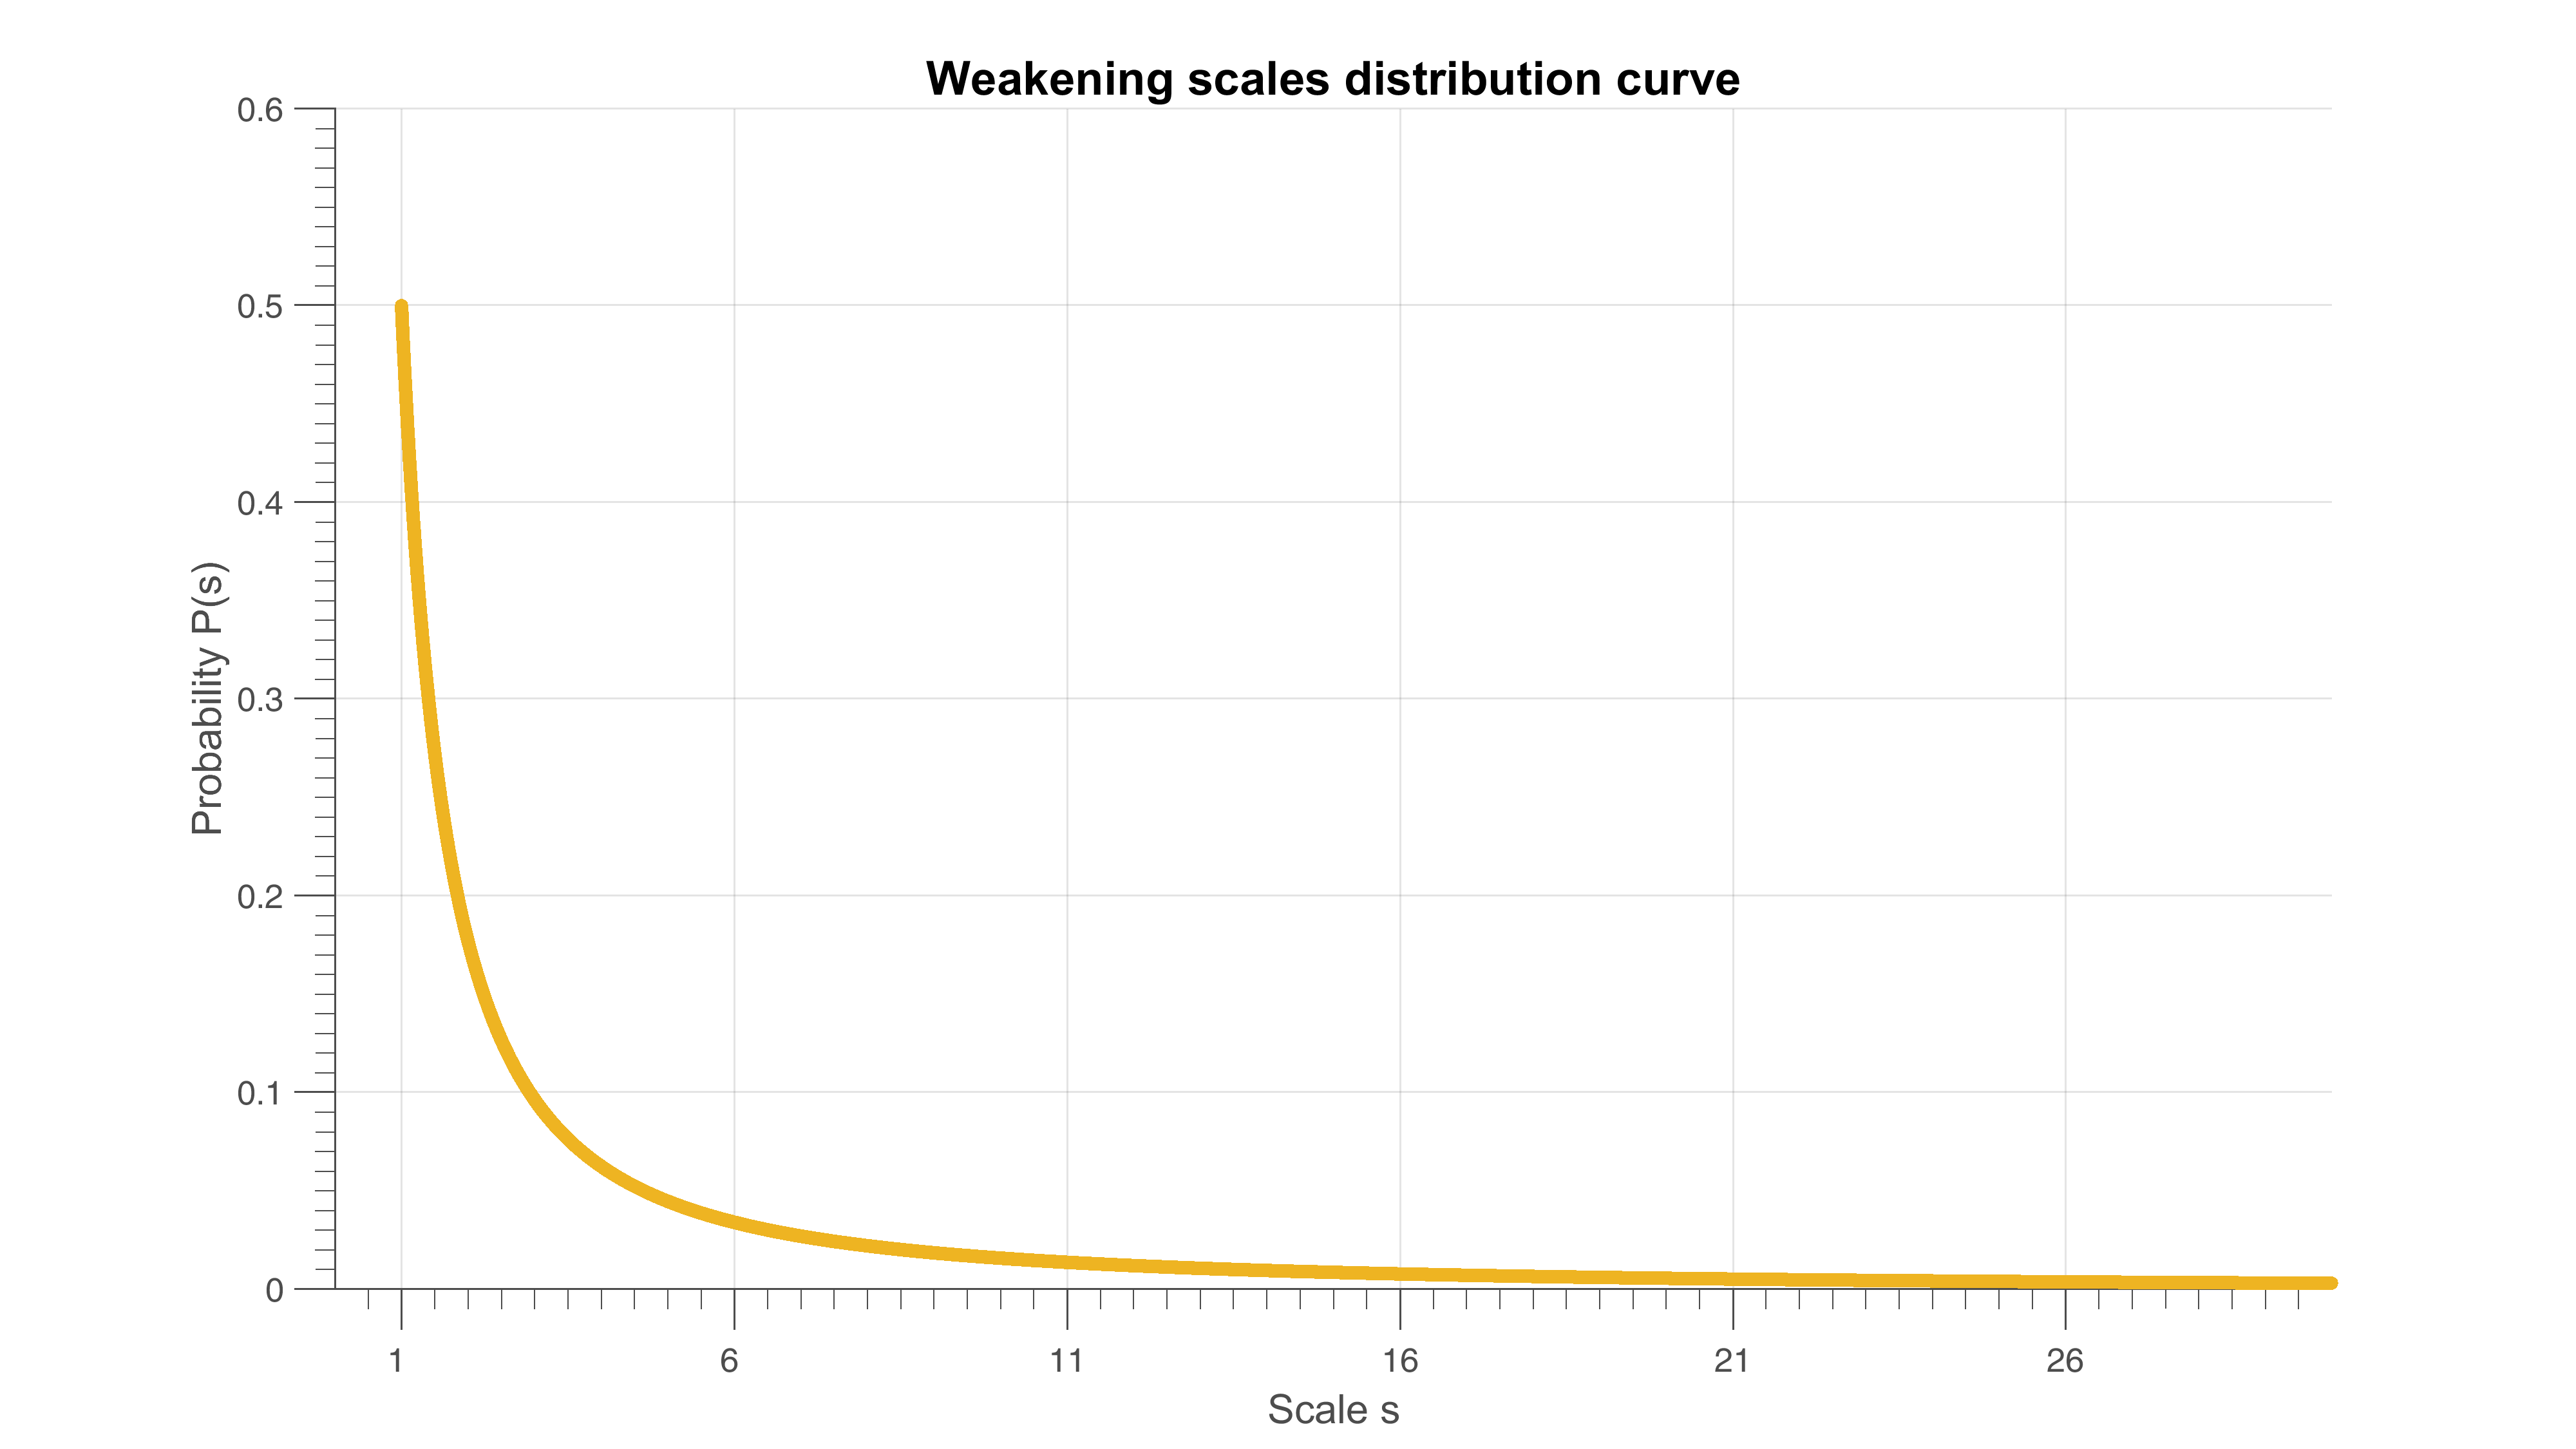
\includegraphics[width=0.9\textwidth]{figures//ps.png} 
	\caption{Weakening scales $s$ probability distribution curve}
	\label{ps}
\end{figure}


\subsection{Yield function with mean stress effect}

Positive mean stress clearly reduces the fatigue life of the material. In design evaluation of multiaxial fatigue with mean stress, a simplified, conservative relation between mean stress and equivalent alternating stress is necessary. We can improve the model by modifying the yield function $\sigma_y$ and the localization tensor.

The idea is to consider as in Maitournam and Krebs\cite{Maitournam2011232} that the yield limit $\sigma_y$ can be reduced in presence of positive mean stress. The mesoscopic yield function can therefore be written as:
\begin{equation}
f\left(s\right)=||\uline{\uline{S}}(s)-\uline{\uline{b}}(s)||+\left( \lambda \Sigma_H-\sigma_y\right) /s\leqslant 0
\label{yieldfun}
\end{equation}
with $\uline{\uline{S}}$ denoting the deviatoric part of the stress tensor at microscale, and $\uline{\uline{b}}(s)$ the corresponding backstress at the same scale. The material remain in elastic regime when $f<0$ and in plastic regime when $f=0$.

\subsection{Local plastic model}
First we should describe the mesoscopic stress state.  The model considers a plastic 
behavior at the mesoscopic scale. The mesoscopic evolution equations are thus:

% \begin{numcases}{}
% 	\dot{\uline{\uline{S}}}(s,M,t)=dev\dot{\uline{\uline{\Sigma}}}(M,t)-\dfrac{E}{1+\nu}\dot{\uline{\uline{\varepsilon}}}^p(s,M,t), & Taylor-Lin scale transition model with unit localization tensor\cite{Bosia201239}.\\
% 	\dot{\uline{\uline{b}}}(s,M,t)=\dfrac{kE}{E-k} \dot{\uline{\uline{\varepsilon}}}^p(s,M,t) , & kinematic hardening model.\\
% 	\dot{\uline{\uline{\varepsilon}}}^p(s,M,t)=\gamma\dfrac{\partial f(s,M,t)}{\partial \uline{\uline{S}}}, & plastic flow rule assuming $\gamma=0$ when $f<0$ and  $\gamma\geqslant0$ when $f=0$.
% \end{numcases}
 
	\begin{equation}
    \dot{\uline{\uline{S}}}(s,M,t)=dev\dot{\uline{\uline{\Sigma}}}(M,t)-\dfrac{E}{1+\nu}\dot{\uline{\uline{\varepsilon}}}^p(s,M,t), 
	\end{equation}
     which defines a Taylor-Lin scale transition model with unit localization tensor\cite{Bosia201239}.
		\begin{equation}
		\dot{\uline{\uline{b}}}(s,M,t)=\dfrac{kE}{E-k} \dot{\uline{\uline{\varepsilon}}}^p(s,M,t), 
		\end{equation}
		which is our kinematic hardening model.
		\begin{equation}
		\dot{\uline{\uline{\varepsilon}}}^p(s,M,t)=\gamma\dfrac{\partial f(s,M,t)}{\partial \uline{\uline{S}}}, 
		\end{equation}
		which is the associated plastic flow rule assuming $\gamma=0$ when $f<0$ and  $\gamma\geqslant0$ when $f=0$.

Here E denotes the Young's modulus and k the hardening parameter. The local dissipated energy rate per volume at weakening scales $s$  is given by the local entropy dissipation:
\begin{equation}
	\dot{w}(s,M,t)=(\uuline{S}-\uuline{b})(s,M,t):\uuline{\dot{\varepsilon}}^p(s,M,t).
	\label{dissipated}
\end{equation}

\section{Construction of an energy based fatigue approach}

In a preliminary step, we will consider a simple macroscopic loading history $\uuline{\Sigma}(M, t)$ which is uniaxial
and time periodic of deviatoric amplitude $S_{max}$, and a Von Mises flow rule to see if we get a prediction of local failure for a number of cycles $N_F$ varying as $\Sigma^{-\beta}.$


\noindent
In uniaxial cyclic loading, there will be 3 kinds of loading patterns, as is shown in \figref{backstress}:

\vspace{6pt}
\begin{enumerate}
	
	\item	Elastic regime, in phase 2 and 4,where $\dot{\uline{\uline{\varepsilon}}}^p(s,M,t)=0$ ,  and $|\uline{\uline{S}}-\uline{\uline{b}}|<\left( \sigma_y-\lambda \Sigma_H\right)/s. $ 
	\vspace{6pt}
	
	\item Plastic regime according to plastic flow rule, with increasing plastic deformation, in phase 5 and 1, where	$\dot{\uline{\uline{\varepsilon}}}^p(s,M,t)=\gamma\dfrac{\uline{\uline{S}}(s)-\uline{\uline{b}}(s)}{||\uline{\uline{S}}(s)-\uline{\uline{b}}(s)||}> 0$ with  $\gamma=\left( dev\dot{\Sigma}\right)\left(\dfrac{kE}{E-k}+\dfrac{E}{1+\nu} \right) ^{-1}$ ,  with $\uline{\uline{S}}-\uline{\uline{b}}=\left( \sigma_y-\lambda \Sigma_H\right)/s$ and $\dot{\uline{\uline{S}}}-\dot{\uline{\uline{b}}}=0.$ 
	\vspace{6pt}
	
	\item Plastic regime in the other direction, in phase 3, there is	$\dot{\uline{\uline{\varepsilon}}}^p(s,M,t)<0$,  then $\uline{\uline{S}}-\uline{\uline{b}}=-\left( \sigma_y-\lambda \Sigma_H\right)/s$ and $\dot{\uline{\uline{S}}}-\dot{\uline{\uline{b}}}=0$ 
	
\end{enumerate}	

\begin{figure}[!h]
	\centering
	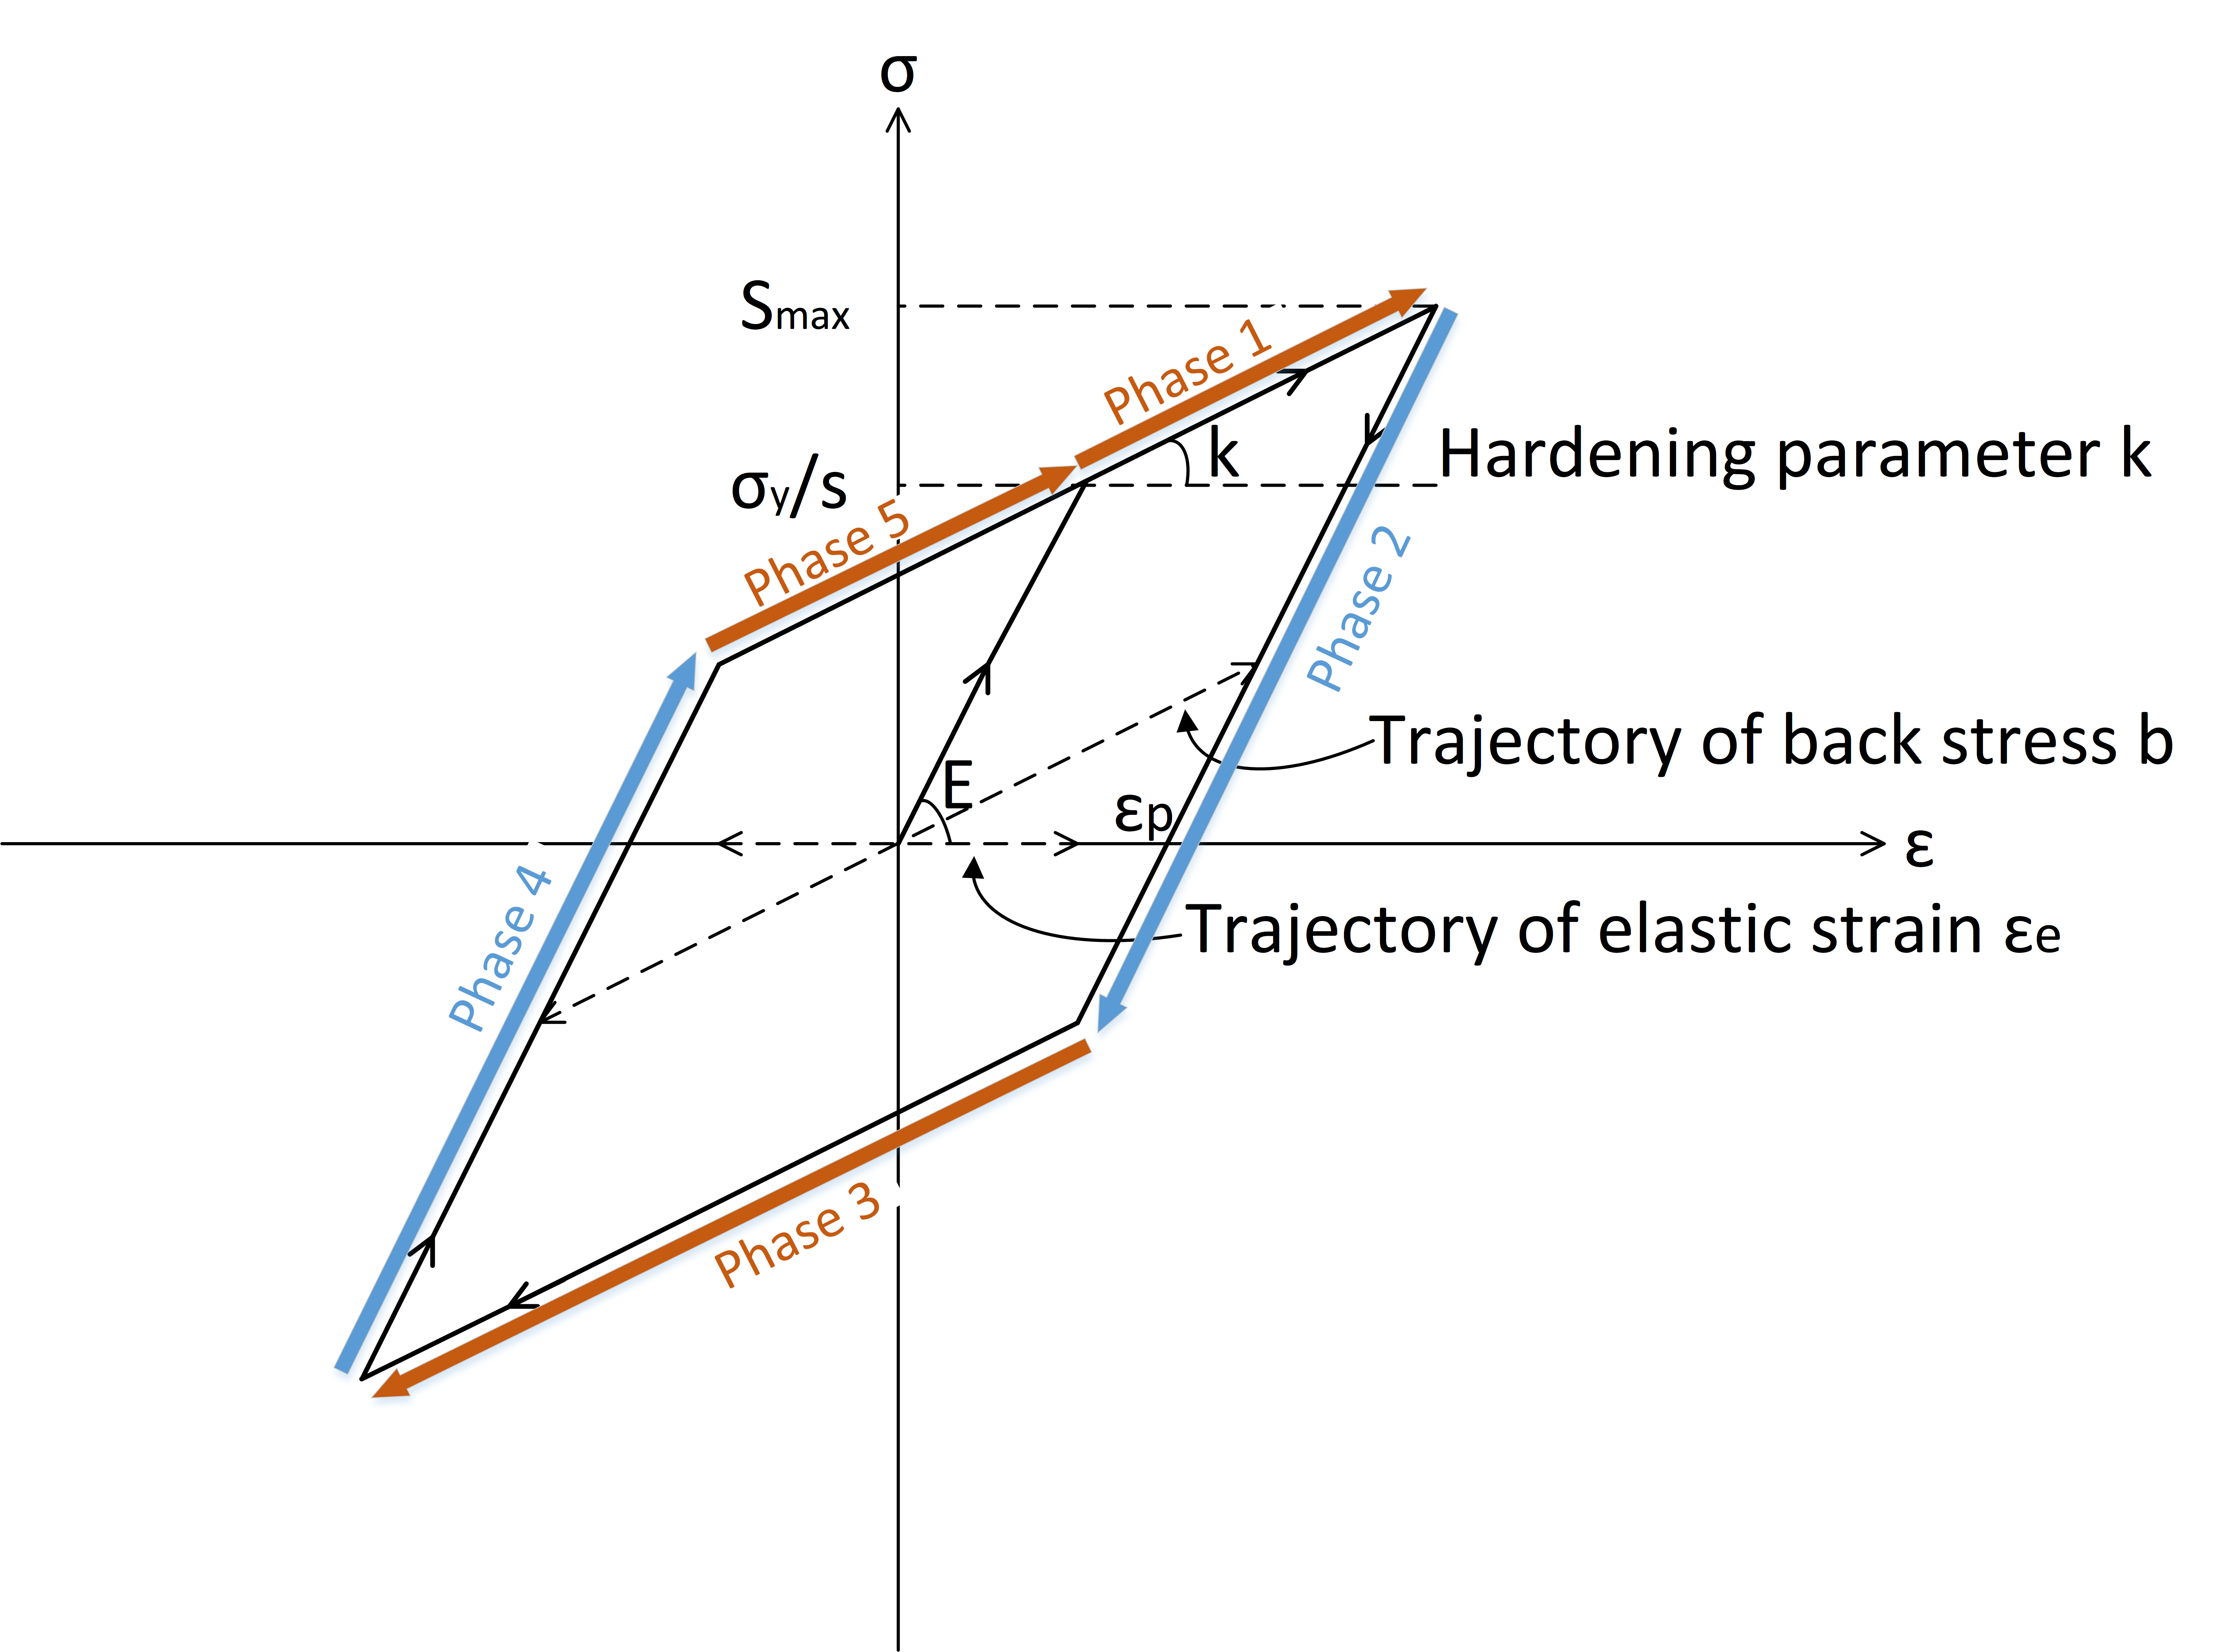
\includegraphics[width=0.9\textwidth]{figures//backstress.png} 
	\caption{Uniaxial load with plastic dissipation}
	\label{backstress}
\end{figure}

In phase 1, a direct analysis yields the energy dissipation at scale $s$:
\begin{equation}dW=(S-b)d\varepsilon^p=\dfrac{(E-k)(1+\nu) }{E(E+k\nu)}\dfrac{\sigma_y-\lambda \Sigma_H}{s}\left(S_{max}-\dfrac{\sigma_y-\lambda \Sigma_H}{s}\right)
\label{dw}
\end{equation}

A similar analysis yields $$dW(phase 1)=dW(phase 5)=\dfrac{1}{2}dW(phase 3).$$

We can then calculate  the local dissipated energy $W$  at point $M$ during one cycle by cumulating the input of all sub-scales with their probabilities \cite{zepeng}.
\begin{equation}
\begin{split}
W_{cyc}&=4\int_{\left( \sigma_y-\lambda \Sigma_H\right) /S_{max}}^{\infty}dW(s,M,t)P(s)ds
\\&=4\int_{\left( \sigma_y-\lambda \Sigma_H\right) /S_{max}}^{\infty}\dfrac{(E-k)(1+\nu) }{E(E+k\nu)}\dfrac{\sigma_y-\lambda \Sigma_H}{s}\left(S_{max}-\dfrac{\sigma_y-\lambda \Sigma_H}{s}\right)\left( \beta-1\right) s^{-\beta}ds
\\&=\dfrac{4(E-k)(1+\nu)\left( \beta-1\right) }{ E(E+k\nu)\beta\left( \beta+1\right) }\dfrac{S_{max}^{\beta+1}}{\left( \sigma_y-\lambda \Sigma_H\right) ^{\beta-1}}.
\end{split}
\label{eq:w}
\end{equation}
 If the dissipated energy accumulates linearly until a failure value $W_F$, we can get directly the time to failure from Eq.\eqref{lineartime}:
\begin{equation}
T_{fail}=N_{F}t_{cyc}=\dfrac{W_F}{W_{cyc}}t_{cyc}=C(S_{max})^{-\beta-1}.
\label{lineartime}
\end{equation}
From Eq.\eqref{eq:w}, we then obtain that the model predicts as expected a power law dependence in function of $S_{max}$.
However, experiments shows that the damage or the energy accumulation of a material evolves non-linearly in time. We should introduce below a method to handle such a nonlinearity.

\section{Nonlinearity of damage accumulation}
\subsection{Energy approach with Chaboche law}
The Chaboche law\cite{lemaitre1990mechanics} is essentially a damage incremental law for cyclic loading of stress intensity $\sigma$ with a deviatoric part ${A}_{\uppercase\expandafter{\romannumeral2}}$ and hydrostatic part $\Sigma_H$, defining the damage increase by:

 \begin{equation}\delta D = \left( 1 -(1-D)^{\gamma+1}\right)^\alpha \left(\frac{{A}_{\uppercase\expandafter{\romannumeral2}}/\left( 1-D\right) }{M(\Sigma_H)}\right)^\gamma \delta N
 \label{chabochemulti}
 \end{equation} 
 which writes equivalently as Eq.\eqref{integration}
   \begin{equation}\delta [1-(1-D)^{\gamma+1}]^{1-\alpha}=(1-\alpha)(\gamma+1)\left(\dfrac{{A}_{\uppercase\expandafter{\romannumeral2}} }{M(\Sigma_H)}\right)^\gamma \delta N=\dfrac{\delta N}{N_F(\sigma)}.
   \label{integration}
   \end{equation}
Here $N_F(\sigma)$ denotes the number of cycles at intensity $\sigma$ to failure as obtained by integration of Eq.\eqref{integration} from $D=0$ to $D=1$.

In our model, in case of a simple uniaxial cyclic loading, we propose to replace $\dfrac{1}{N_F(\sigma)}$ which is the relative unit increment of cycles by $\dfrac{W_{cyc}}{W_F}$, yielding the nonlinear damage incremental law:
	\begin{equation}
	\delta[1-(1-D)^{\gamma+1}]^{1-\alpha}=\dfrac{W_{cyc}}{W_F}\delta N.
\label{integrationW}
\end{equation}
This is a nonlinear law but used with a constant $\alpha$, there will be no sequence effect. In other words,
 when applying two successive cycles of different intensities, the failure will occur at the same number of cycles whatever the order of the loading(high then low versus low then high).
 
\subsection{Generalized damage accumulation}
Formula \eqref{integration} is a general accumulation law which can be applied for any cyclic loading sequence provided that we can identify the multiscale value of the dissipated energy per cycle. 

But the notion of cycle itself may be hard to identify for general loadings. The idea is then to replace the relative increment of dissipated energy per cycle by the relative increment of dissipated energy per unit time, yielding:
\begin{equation}
\delta [1-(1-D)^{\gamma+1}]^{1-\alpha}=\dfrac{\dot{W}}{W_F}\delta t.
\label{dt}
\end{equation}

In a general loading case, $\dot{W}$ is to be computed. By integrating Eq.\eqref{dissipated} over all microscales, we get:
\begin{equation}\dot{W}(M,t)=\int_{s=1}^{\infty}\dot{w}(s,M,t)P(s)ds=\int_{s=1}^{\infty}\left(\uuline{S}-\uuline{b} \right) (s,M,t):\uuline{\dot{\varepsilon}^p}(s,M,t)P(s)ds.\label{Wdot}
\end{equation}
The evolution of $\uuline{S}$, $\uuline{b}$ and $\uuline{\dot{\varepsilon}^p}$ are given in section 1.4. Equation \eqref{dt} and \eqref{Wdot} are therefore our proposed damage law.

\section{Loop on time and scales}
\subsection{Integration rules for $\dot{W}$ and $\delta D$}
Our first approach takes one cycle as unit time. We compute analytically the energy dissipation at each scale during this cycle. The method is valid for simple loading history and which includes the integration on all weakening scales. The damage $D$ is accumulated after each cycle.

However, there are certain limitations of this method. Firstly we need a load history decomposition in cycles. Secondly in real life the perfect close loop cycle is hardly applicable.

Thus we propose in Eq.\eqref{dt} a more general method which can be integrated by a step by step strategy. We compute numerically the dissipation at different scales using an implicit Euler time integration of the constitutive laws of section 1.4. After which we make a numerical integration on different scales. Then we can update the damage and go to next time step. 

Instead of doing the scale integration directly which can be difficult for complex loading, the Gaussian Quadrature rule with Legendre points is used to give the value of local dissipated energy rate.

To use the Gaussian quadrature rule the limit range of integral must be from $-1$ to $1$, while the total dissipated energy  is expressed by integrating all the weakening scale $s$ ranging from 1 to infinity with their occurrence probabilities:
$$\dot{W}=\int_{1}^{\infty}\dot{w}(s) (\beta-1)(s)^{-\beta}ds.$$

\noindent
To change the limit range of integral from $[1,\infty]$ to $[1,0]$ we take as new integration variable
$u(s)= s^{-p}$ with $p=\beta-1$, yielding $u(1)=1$ and  $u(\infty)=0$ with
$$du=-ps^{-p-1}ds$$ 
that is
$$du=(-\beta+1) s^{-\beta}ds=(-\beta+1)s^{-\beta} ds.$$
Therefore the dissipated energy summed on all scales is:
\begin{equation}
\begin{split}
\dot{W}&=\int_{1}^{\infty}\dot{w}(s) (\beta-1)(s)^{-\beta}ds
\\&=\int_{1}^{0}\dot{w}\left( u^{\frac{1}{1-\beta}}\right) (\beta-1) \frac{1}{-\beta+1}du
\\&=\int_{0}^{1}\dot{w}\left( u^{\frac{1}{1-\beta}}\right) (\beta-1) \frac{1}{\beta-1}du
\\&=\int_{0}^{1}\dot{w}\left( u^{\frac{1}{1-\beta}}\right)du
\\&=\frac{1}{2}\int_{-1}^{1}\dot{w}\left[  \left( \frac{x+1}{2}\right) ^{\frac{1}{1-\beta}}\right] dx
\end{split}
\label{allscale}
\end{equation}
if we set $u=\dfrac{x+1}{2}$.

So the dissipated energy rate integrated over all scales takes the form of Eq.\eqref{allscalerate}:
\begin{equation}
\dot{W}=\frac{1}{2}\int_{-1}^{1}\dot{w}\left[  \left( \frac{x+1}{2}\right) ^{\frac{1}{1-\beta}},t\right] dx\approx\frac{1}{2}\sum_{i}\omega_id\dot{w}\left[  \left( \frac{x_i+1}{2}\right) ^{\frac{1}{1-\beta}},t\right],
\label{allscalerate}
\end{equation}
where $\omega_i$ and $x_i$ are respectively the weights and nodes of the Gauss Legerndre integration rule used for the numerical integration. In this work, we used 25 points\cite{legendre}.

After changing the integration limit, $\left( \dfrac{x+1}{2}\right) ^{\frac{1}{1-\beta}}$ represents the weakening scale $s$. 

Damage accumulation is deduced from Eq.\eqref{dt}:
\begin{equation}
g_{n+1}=g_n+\dfrac{\dot{W}dt}{W_F}
\label{damage}
\end{equation}

with $g_n=\left[ 1-\left( 1-D_{n}\right)^{\gamma+1} \right]^{1-\alpha}$.

We upgrade the damage step by step following Eq.\eqref{damage}. When $D$ reaches one, the material fails. 

\subsection{Regime determination under multiple scales}
The material could be both in elastic and plastic regime under different scales. To be more elaborate, we reuse the fundamental equations in different regimes. At scale $s$, we have a dissipation rate given by:
$$\dot{w}(s)=\left( \uline{\uline{S}}-\uline{\uline{b}}\right):\dot{\uline{\uline{\varepsilon}}}^p, $$
which differs between plastic and elastic regime.

\vspace{6pt}
\noindent
\textbf{Elastic regime:}

\vspace{6pt}
\noindent
There we have
$\dot{\uline{\uline{\varepsilon}}}^p=0$, $\dot{\uline{\uline{b}}}=0$ and $\dot{\uline{\uline{S}}}=dev\dot{\uline{\uline{\Sigma}}}$, so
$$\dot{\uline{\uline{S}}}-\dot{\uline{\uline{b}}}=dev\dot{\uline{\uline{\Sigma}}},$$ 
yielding
\begin{equation}
\left( \uline{\uline{S}}-\uline{\uline{b}}\right) (t+dt)=\left( \uline{\uline{S}}-\uline{\uline{b}}\right) (t)+dev\dot{\uline{\uline{\Sigma}}}dt:=\left(  \uline{\uline{S}}-\uline{\uline{b}}\right)_{trial}(s,t+dt).
\label{trial}
\end{equation}
We are in elastic regime at scale $s$ as long as we satisfy
$$\left( \uline{\uline{S}}-\uline{\uline{b}}\right) (t+dt)\leqslant\left( \sigma_y-\lambda \Sigma_H\right)/s.$$

\vspace{6pt}
\noindent
\textbf{Plastic regime:}

\vspace{6pt}
\noindent
When we leave elastic regime at scale s, we have:
\begin{numcases}{}
\dot{\uline{\uline{\varepsilon}}}^p=\gamma\dfrac{\uline{\uline{S}}-\uline{\uline{b}}}{\left| \left|\uline{\uline{S}}-\uline{\uline{b}}\right| \right|}, \gamma>0, & plastic   flow,\\
\left| \left|\uline{\uline{S}}-\uline{\uline{b}}\right| \right|=\left( \sigma_y-\lambda \Sigma_H\right)/s, & yield   limit,\\
\left( \uline{\uline{S}}-\uline{\uline{b}}\right) :\left( \dot{\uline{\uline{S}}}-\dot{\uline{\uline{b}}}\right) =0, & yield   limit   time invariance,\\
\dot{\uline{\uline{b}}}=\dfrac{kE}{E-k}\dot{\uline{\uline{\varepsilon}}}^p, & kinematic   hardening  rule,\\
\dot{\uline{\uline{S}}}=dev\dot{\uline{\uline{\Sigma}}}-\dfrac{E}{1+\nu} \dot{\uline{\uline{\varepsilon}}}^p, & localisation  rule.
\end{numcases}
 
In all cases, we get(see annex 'Multi-dimensional analysis')
\begin{equation}
\left( \uline{\uline{S}}-\uline{\uline{b}}\right) (s,t+dt)=\dfrac{\left( \uline{\uline{S}}-\uline{\uline{b}}\right)_{trial} (s,t+dt)}{1+\eta},
\end{equation}

with $$\eta=max\left\lbrace \underbrace{0}_{elastic\; regime}, \underbrace{\dfrac{\left| \left|\uline{\uline{S}}-\uline{\uline{b}}\right| \right|_{trial}}{\left( \sigma_y-\lambda \Sigma_H\right)/s}-1}_{plastic \; regime\; when\; this\; number\; is\; positive}\right\rbrace, $$

$$\left( \uline{\uline{S}}-\uline{\uline{b}}\right)_{trial} (s,t+dt)=\left( \uline{\uline{S}}-\uline{\uline{b}}\right)(s,t)+dev\dot{\uline{\uline{\Sigma}}}(t)dt.$$

 That is to say, when the structure is in elastic regime at time $t$ and scale $s$, we have $\left( \uline{\uline{S}}-\uline{\uline{b}}\right)(s,t)=\left( \uline{\uline{S}}-\uline{\uline{b}}\right)_{trial} (s,t)$. Otherwise, if  the norm of $\left( \uline{\uline{S}}-\uline{\uline{b}}\right)_{trial} (s,t)$ is greater than the local yield limit $\left( \sigma_y-\lambda \Sigma_H\right)/s$, $\left( \uline{\uline{S}}-\uline{\uline{b}}\right)(s,t)$ will be projected on the yield limit. 
 
Knowing the distinction between elastic and plastic regime under multiple scales, we compute the general expression of the dissipated energy rate.
\begin{equation}
\dot{w}=\left( \uline{\uline{S}}-\uline{\uline{b}}\right) :\dot{\uline{\uline{\varepsilon}}}^p=\gamma\dfrac{ \sigma_y-\lambda \Sigma_H}{s}.
\label{w}
\end{equation}

From Eq.\eqref{eta} and Eq.\eqref{eta2} in annex, we get:

\begin{equation}E\gamma dt=\left\langle \left| \left|\uline{\uline{S}}-\uline{\uline{b}}\right| \right|_{trial}-\dfrac{\sigma_y-\lambda \Sigma_H}{s}\right\rangle /\left(\dfrac{1}{1+\nu}+\dfrac{k}{E-k} \right)=\left\langle \left| \left|\uline{\uline{S}}-\uline{\uline{b}}\right| \right|_{trial}-\dfrac{\sigma_y-\lambda \Sigma_H}{s}\right\rangle\dfrac{(E-k)(1+\nu) }{(E+k\nu)},
\label{gamma}
\end{equation}
where $\langle$ $\rangle$ is Macaulay bracket symbol defined as $\langle m\rangle=0$ if $m\leqslant0$, otherwise $\langle m\rangle=m$.

We replace $\gamma$ deduced from Eq.\eqref{gamma} in Eq.\eqref{w} to give the expression of local energy dissipation rate at scale $s$:
\begin{equation}
\dot{w}dt=\dfrac{(E-k)(1+\nu) }{E(E+k\nu)}\left\langle  \left| \left|\uline{\uline{S}}-\uline{\uline{b}}\right| \right|_{trial}-\dfrac{\sigma_y-\lambda \Sigma_H}{s}\right\rangle \dfrac{\sigma_y-\lambda \Sigma_H}{s}.
\label{dW}
\end{equation}

With Eq.\eqref{allscalerate}, the final expression of energy dissipation $W$ during time step $dt$ writes:

\begin{equation}
  \begin{split}
W&=\dot{W}dt
\\&=\frac{1}{2}\sum_{i}\omega_i\dot{w}\left[  \left( \frac{x+1}{2}\right) ^{\frac{1}{1-\beta}}\right]dt
\\&=\dfrac{(E-k)(1+\nu) }{2E(E+k\nu)}\sum_{i}\omega_i\left\langle  \left| \left|\uline{\uline{S}}-\uline{\uline{b}}\right| \right|_{trial}-\dfrac{\sigma_y-\lambda \Sigma_H}{\left( \dfrac{x_i+1}{2}\right) ^{\frac{1}{1-\beta}}}\right\rangle \dfrac{\sigma_y-\lambda \Sigma_H}{\left( \dfrac{x_i+1}{2}\right) ^{\frac{1}{1-\beta}}}.
  \end{split}
\label{finaldw}
\end{equation}


We have the damage accumulation deduced in Eq.\eqref{damage}:
$$g_{n+1}=g_n+\dfrac{\dot{W}dt}{W_F}=g_n+\dfrac{W}{W_F},$$
with $D_n=\left[1-\left(1-g_n^{\frac{1}{1-\alpha}} \right)^{\frac{1}{\gamma+1}}  \right]. $
 
 Now we are able to put these formula into numerical tests.
 
\section{Test on different load histories}
\subsection{One dimensional application to simple cyclic data}
The test is first performed on a sinusoidal axial load $\Sigma=Csin(t)$ with parameters in Table.\ref{Sin}, giving a deviatoric amplitude $S_{max}=\sqrt{\dfrac{2}{3}}C$.
\begin{table}[!h]
	\centering
	\begin{tabular}{ll}
		\hline
		\textbf{Parameters}                                         & \textbf{Value}                    \\ \hline
		Load                                                              & $\Sigma=5e8sin(t)$ Pa                  \\
		Young's modulus                                             & $E=2e11$ Pa                       \\
		Hardening parameter                                         &  $k=6e8$ Pa \\
		Weakening scales distribution exponent                      & $\beta=3$                             \\
		Hydrostatic pressure sensitivity                            & $\lambda=0.5$                     \\
		Macroscopic yield stress                                    & $\sigma_y=6.38e8$ Pa              \\
		Material parameter from Chaboche law(Wohler curve exponent) & $\gamma=0.5$                        \\
		Non-linearity of damage accumulation & $\alpha=0.5$                        \\
		Initial damage                                              & $D=0$                          \\
		Initial time                                                & $t=0$ s                            \\
		Dissipated energy to failure per unit volume                & $W_F=3e6$ J                       \\
		Looping step                                           & 1 s              \\ \hline
	\end{tabular}
		\caption{Material parameters in a simple cyclic load }
		\label{Sin}
\end{table}

We use matlab to realize our analytical method. We plot $\left\|  \uline{\uline{S}}-\uline{\uline{b}}\right\|_{trial}$ and $\left\|  \uline{\uline{S}}-\uline{\uline{b}}\right\|$ for two different scales($s_1=21.21657929229650$ and $s_8=2.176132808422946$) in \figref{trialsin}.
\begin{figure}[!h]
	\centering
	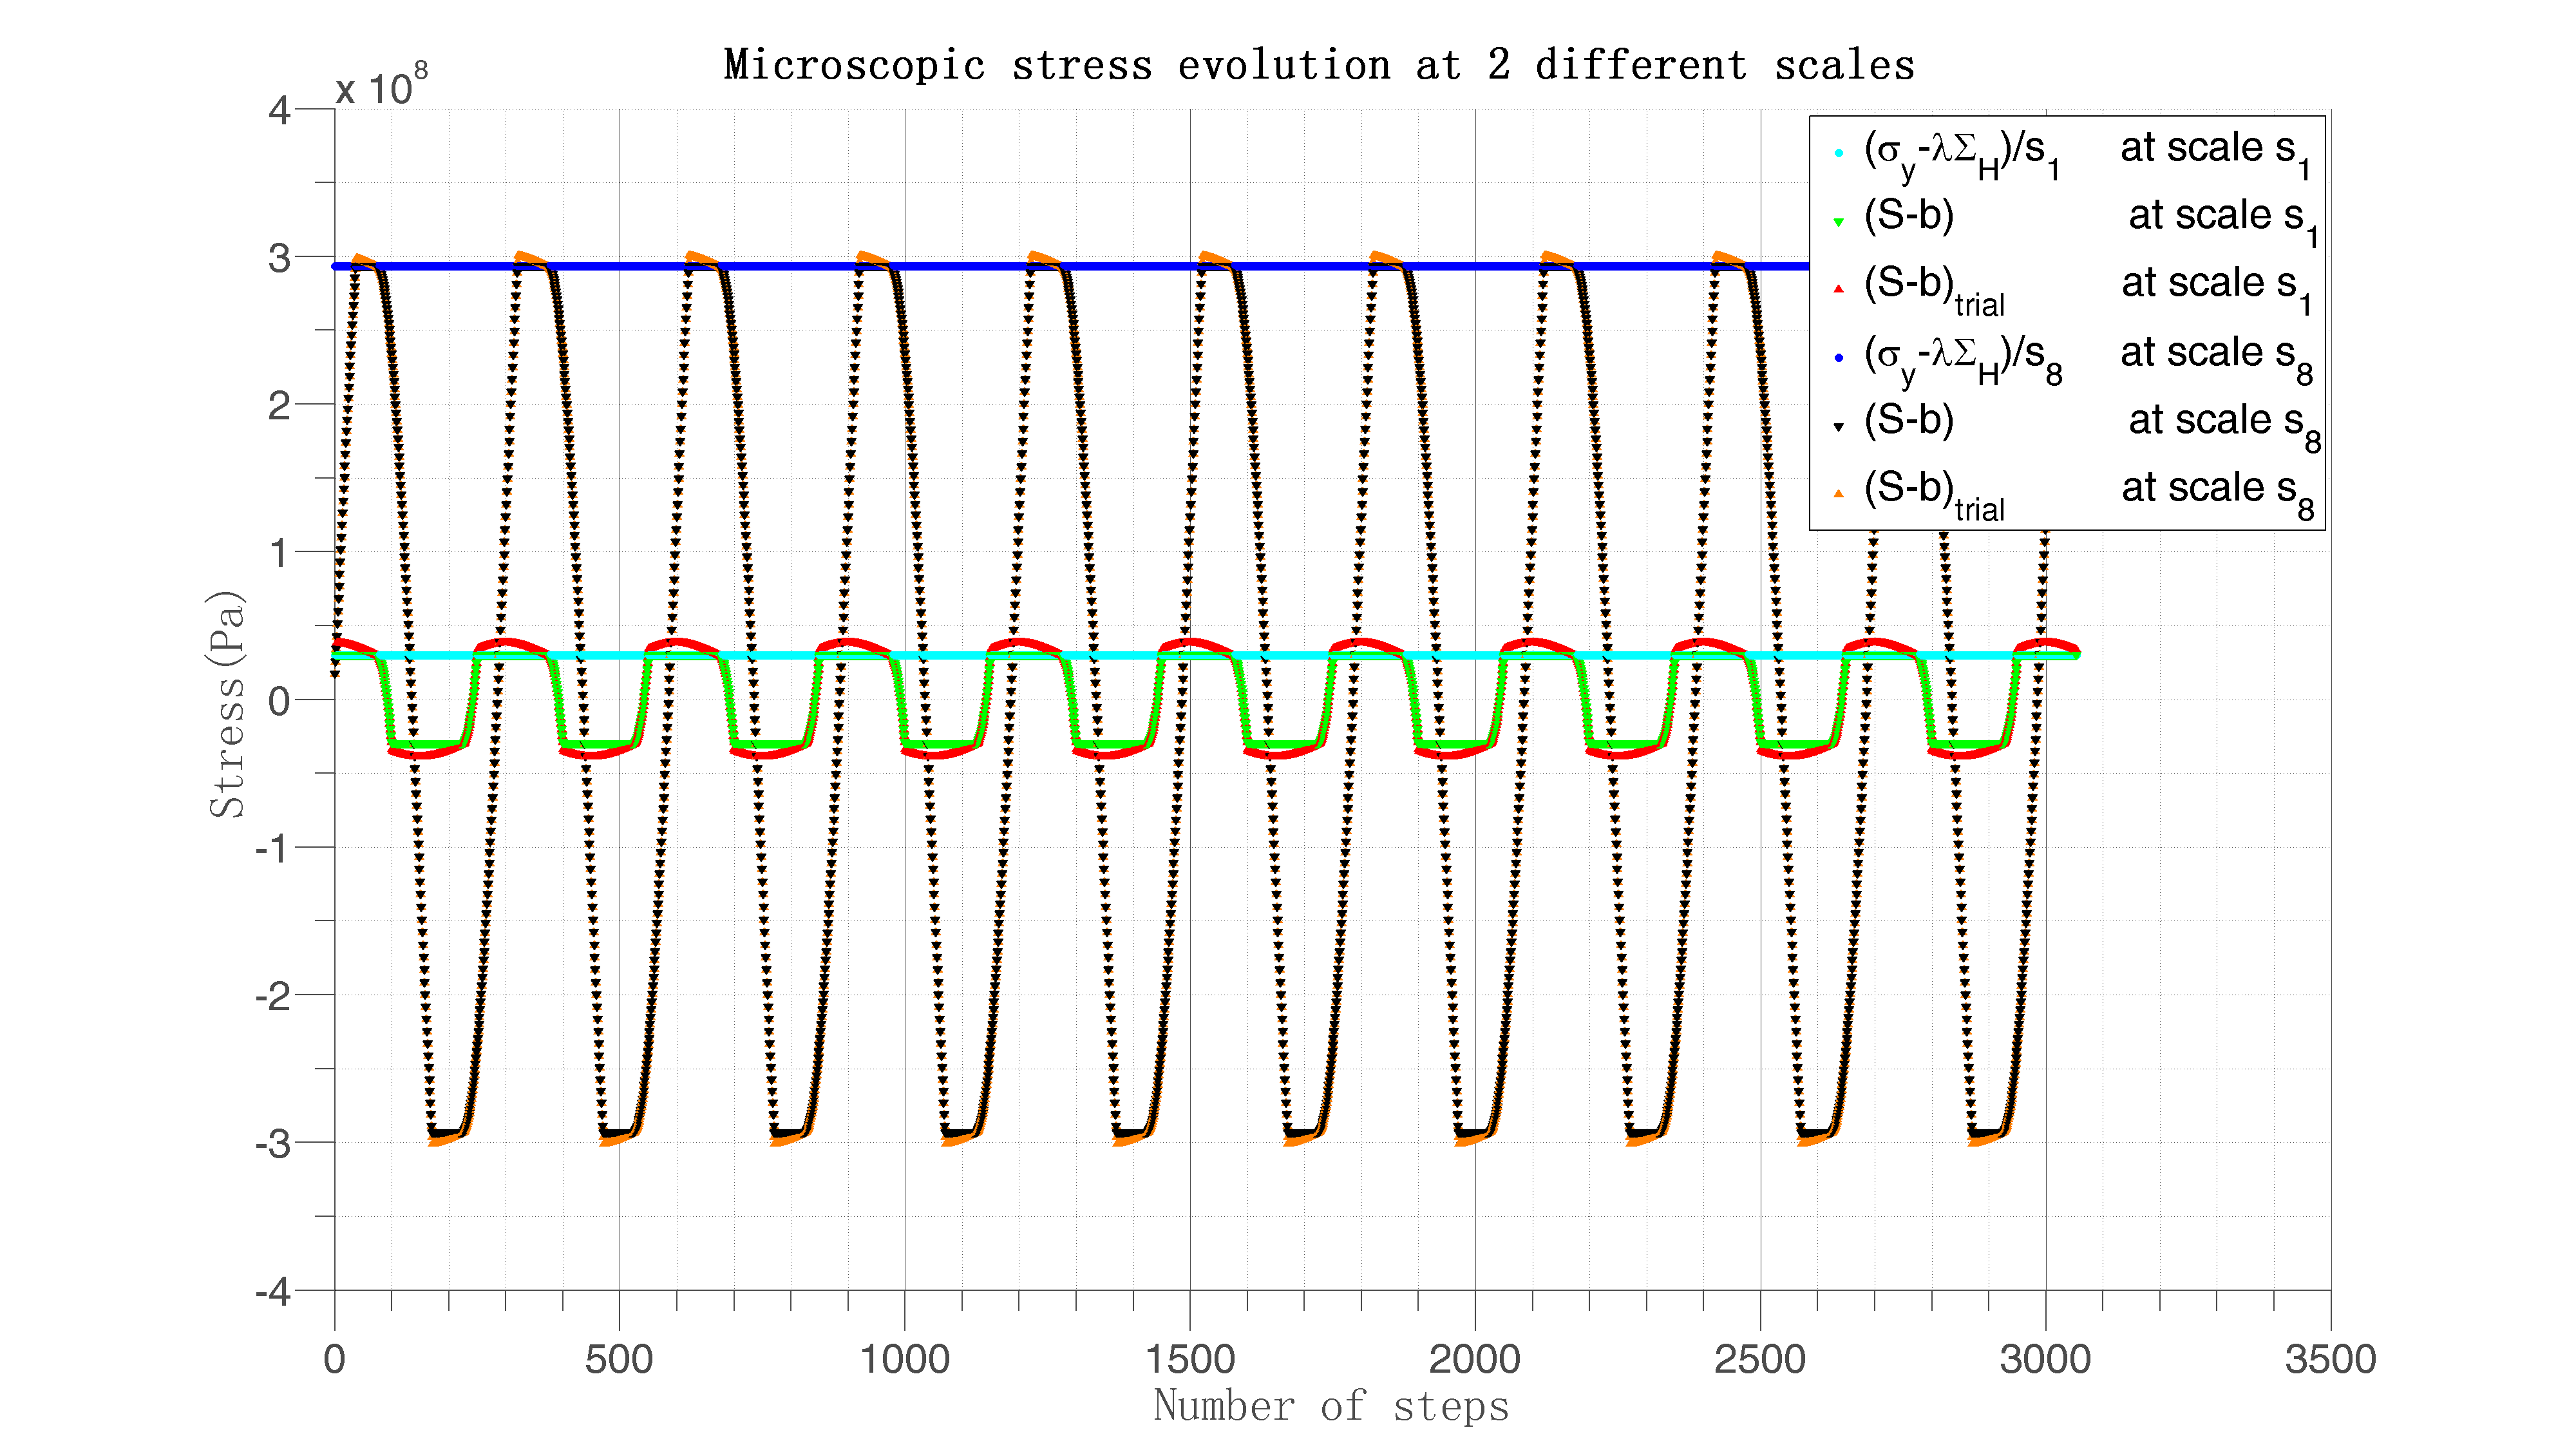
\includegraphics[width=\textwidth]{figures//trialsin.png} 
	\caption{Microscopic $\left(  \uline{\uline{S}}-\uline{\uline{b}}\right)_{trial}$ and $\left( \uline{\uline{S}}-\uline{\uline{b}}\right)$ evolution with time under different weakening scales in sinusoidal load}
	\label{trialsin}
\end{figure}

The nonlinearity is determined by 
$$\alpha=1 - a\left\langle \dfrac{\max\limits_{t}\sqrt{J_{2,a}}(t)+a_c{P_{max}(t)}-b_c}{ \sigma_{u} - 2\max\sqrt{J_{2,a}}}\right\rangle,$$ 
 which is predominated by Crossland criterion, for simplicity we take $\alpha$ as a constant. The damage evolves like in \figref{damsin}, where we compare the damage evolution as predicted by the cycle accumulation Eq.\eqref{eq:w} and by the numerical strategy of section 4.

\begin{figure}[!h]
	\centering
	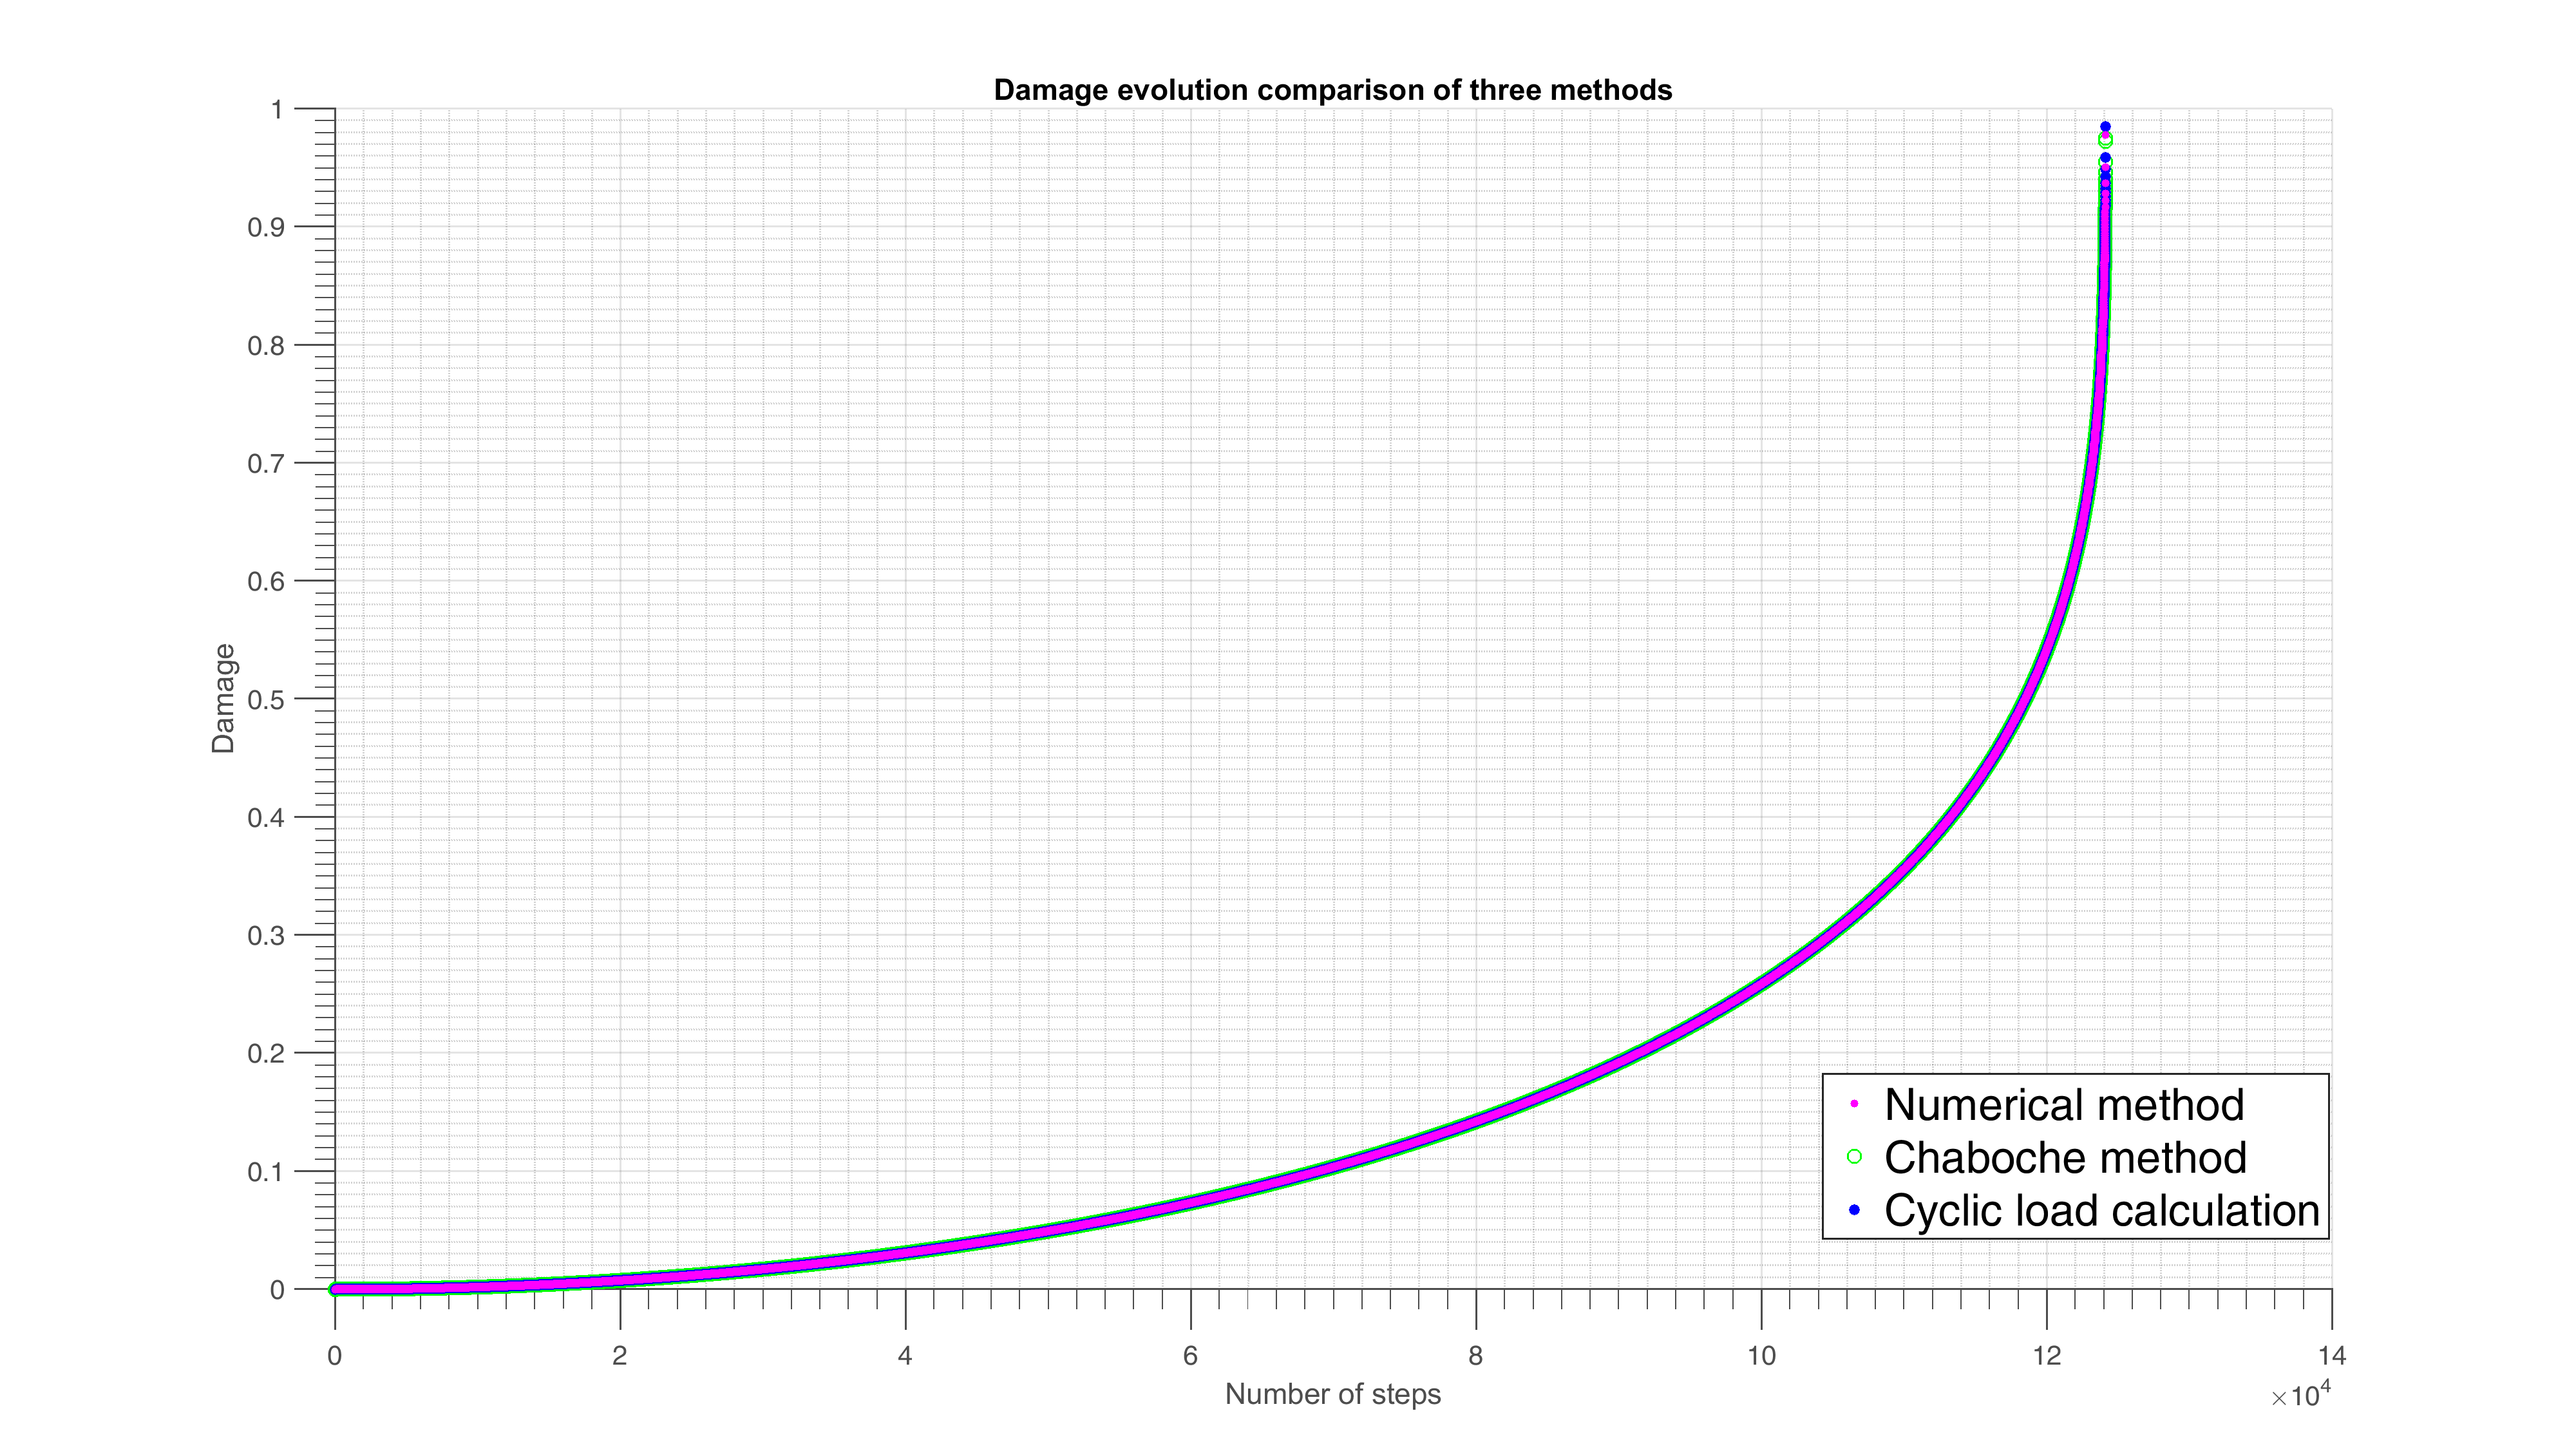
\includegraphics[width=\textwidth]{figures//damagesin.png} 
	\caption{Damage evolution with time under sinusoidal load with two different methods}
	\label{damsin}
\end{figure}

Now we compare the result to the one demonstrated in \figref{backstress}. The first cycle has 3 phases which have the energy loss identical to phase 1. The following cycles each have 4 times energy loss as phase 1. We can see from \figref{NCdiff100} and \figref{NCdiff300} the difference between cyclic load calculation and numerical method as function of time(time step=1/5000s and 1/15000s separately). Because the step by step damage accumulation grows in a power law, so the amplitude of difference grows with time. However, the difference between the two methods swing around 0 and from \figref{damsin} we can see the difference is not symmetrical, we could consider the numerical method converges in cyclic load calculation method.

\begin{figure}[!h]
	\centering
	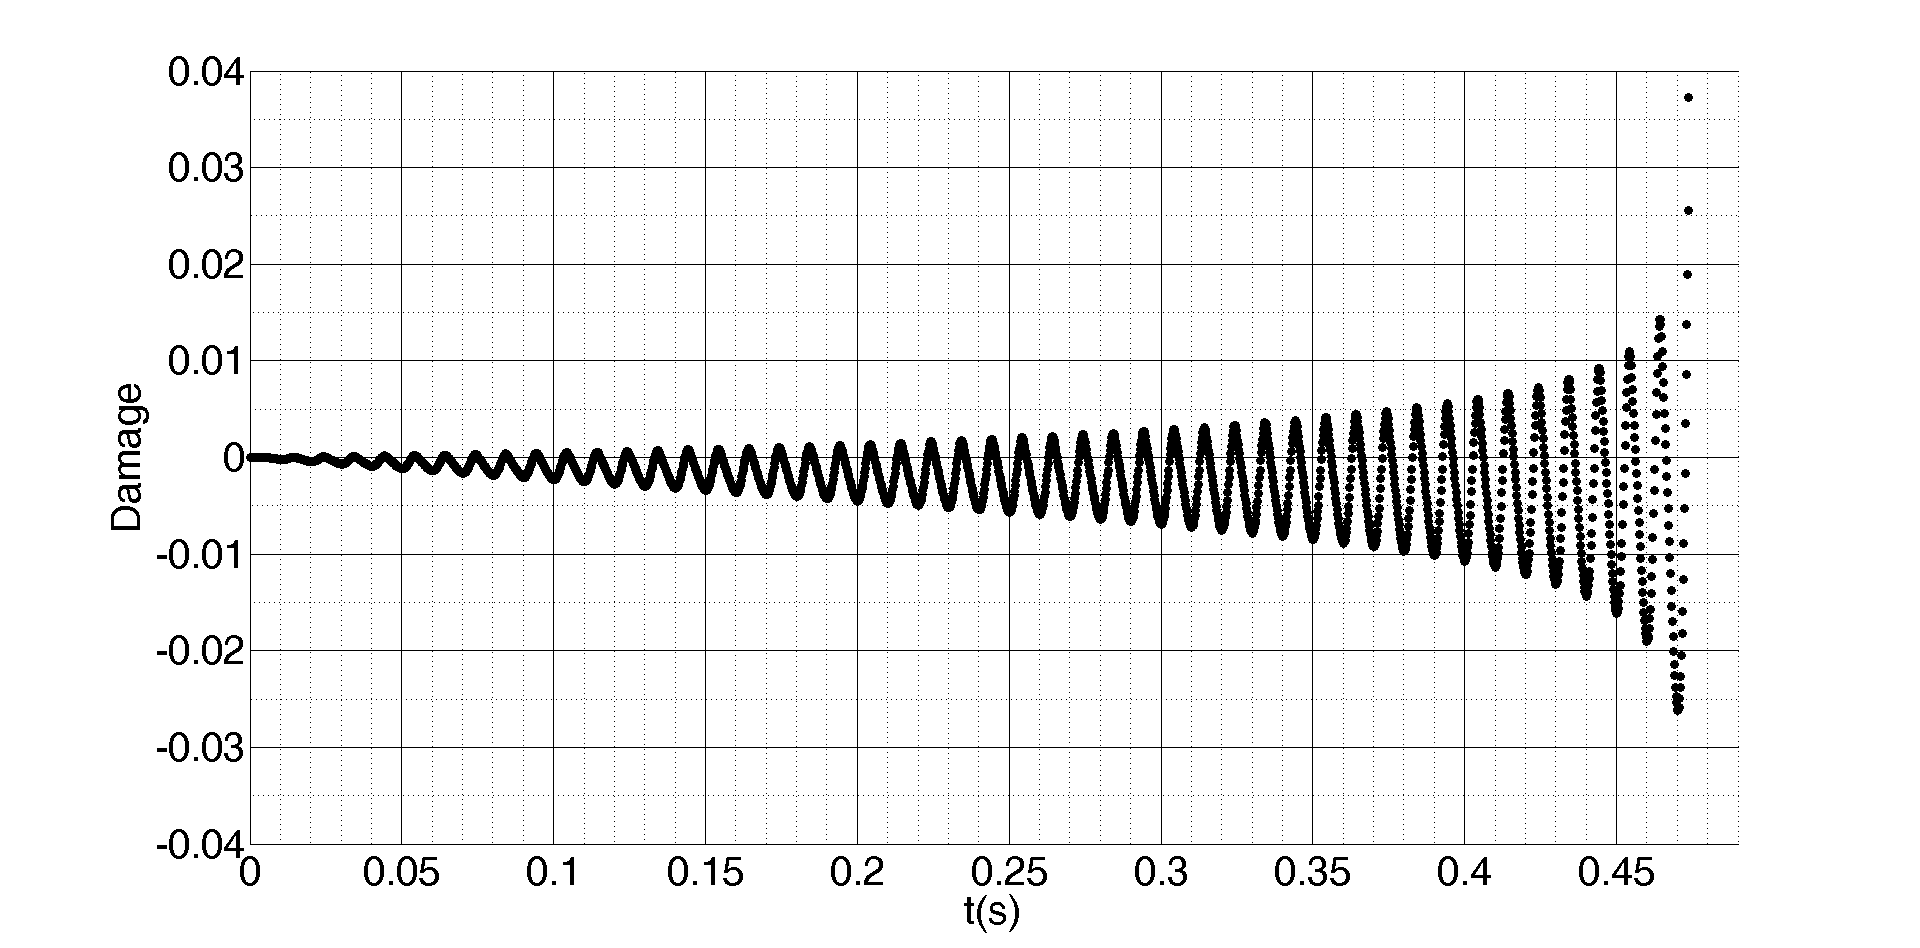
\includegraphics[width=\textwidth]{figures//NCdiff100.png} 
	\caption{Difference between cyclic load calculation and numerical method as function of time(time step=1/5000s)}
	\label{NCdiff100}
\end{figure}
\begin{figure}[!h]
	\centering
	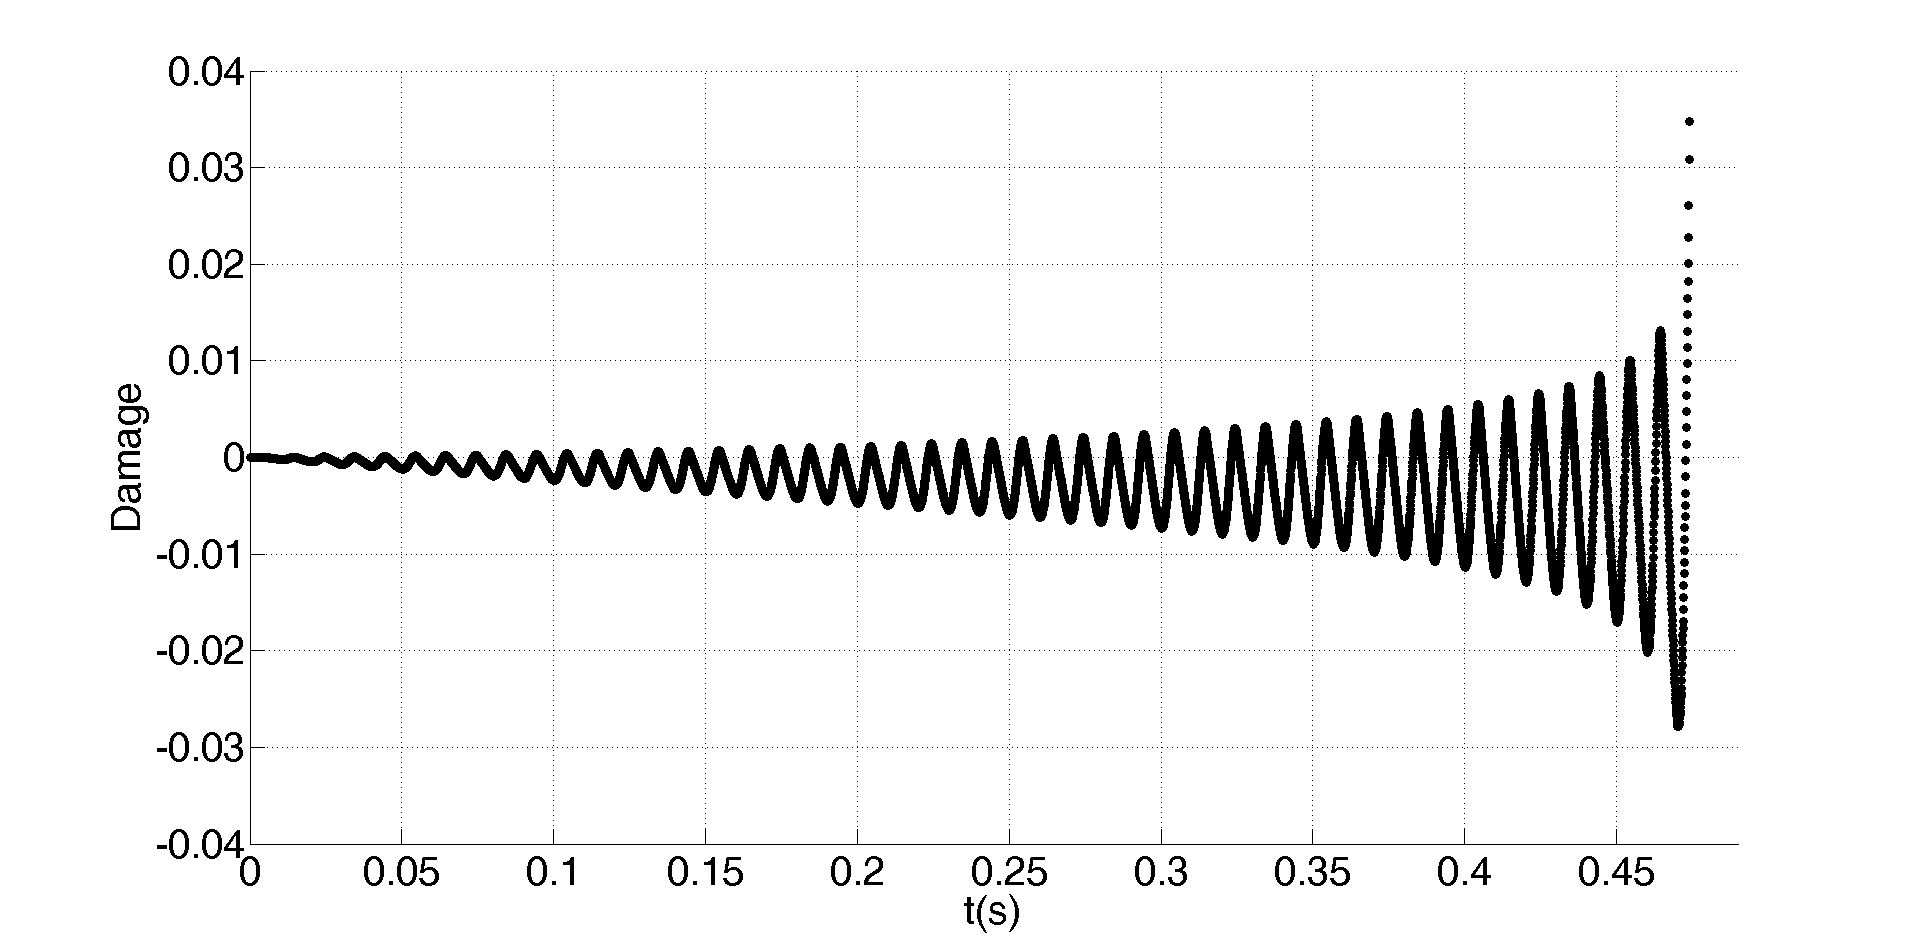
\includegraphics[width=\textwidth]{figures//NCdiff300.png} 
	\caption{Difference between cyclic load calculation and numerical method as function of time(time step=1/15000s)}
	\label{NCdiff300}
\end{figure}
The cyclic load calculation is only valid for very simple such as proportional loading in fatigue, nevertheless it can still be used as a comparison group to verify the numerical results. The outcome seems satisfactory. Hence, to be more general for any loading history, we adopt the numerical method.


\subsection{One dimensional application to PSA data}
In this test, we reconstruct a unidimensional macroscopic stress history from recorded force data proposed by PSA group. 
\begin{figure}[!h]
	\centering
	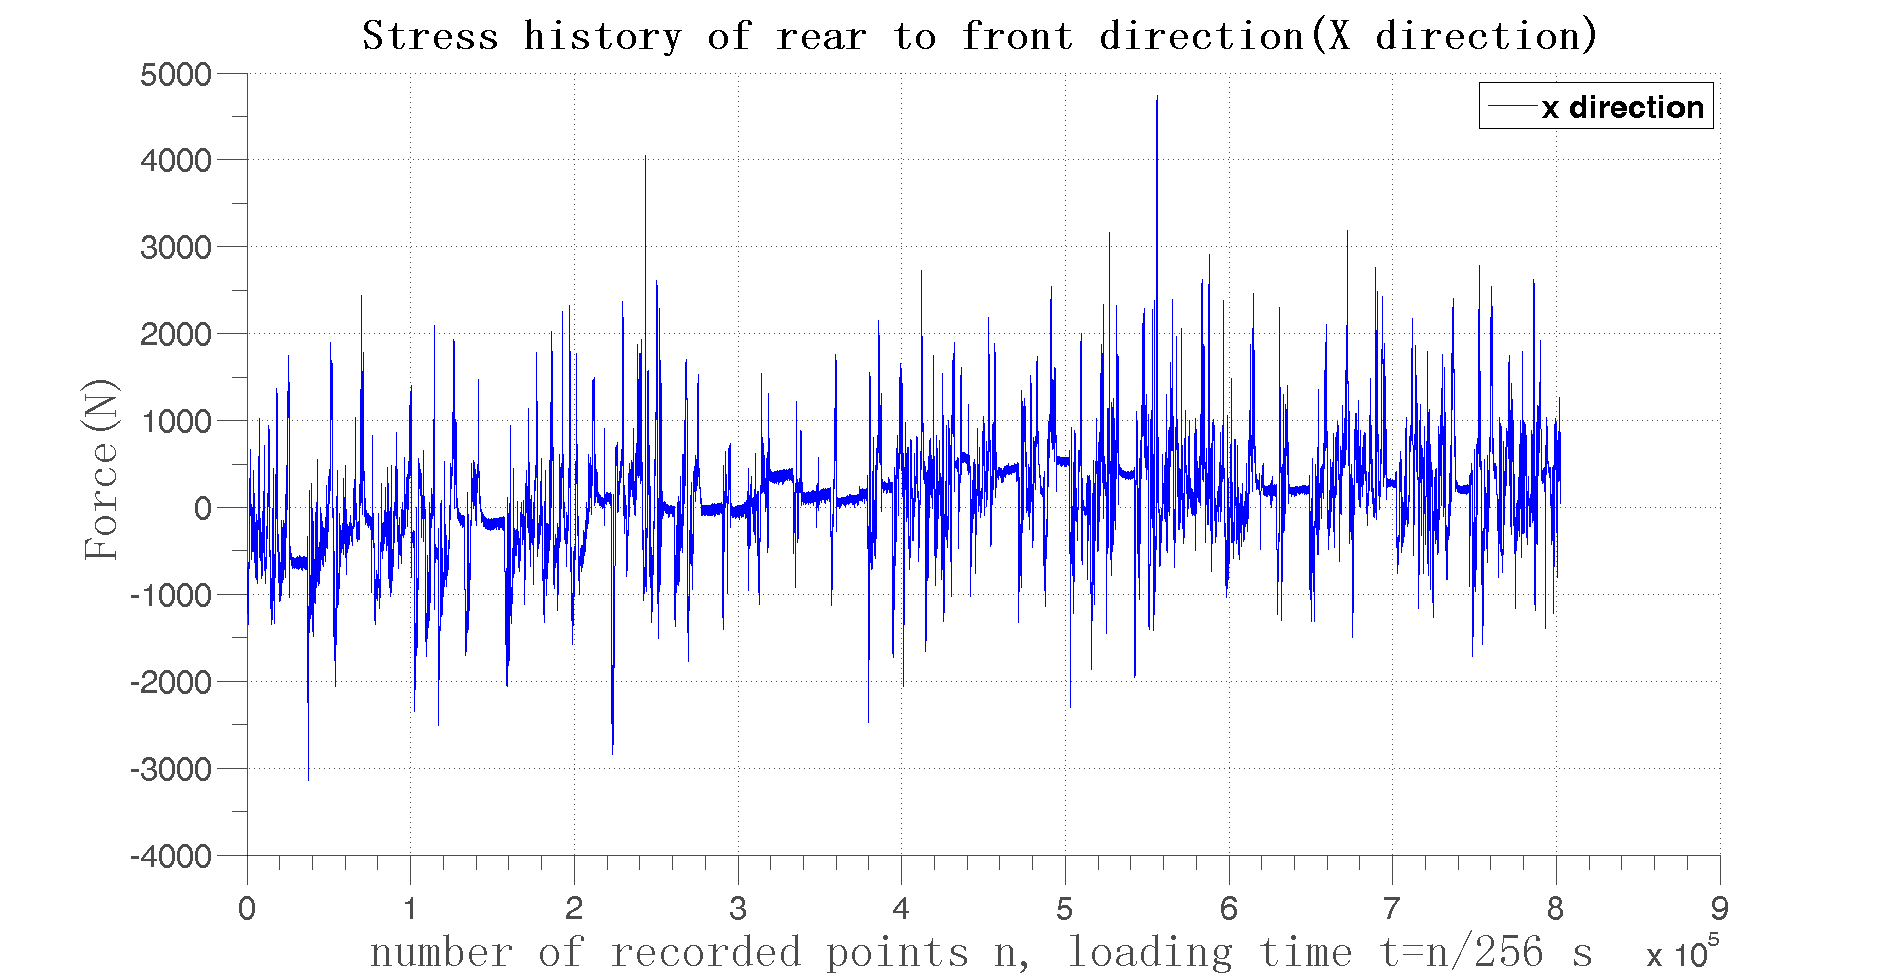
\includegraphics[width=\textwidth]{figures//x.png} 
	\caption{Loading history of X direction, force vs the record index n, with 256 sample recorded per second}
	\label{x}
\end{figure}

The sample recording rate is 256 per second. In order to accumulate damage using very small steps, we have created 10 additional points between every 2 recorded points by linear interpolation. So the sample rate is $256*10$ per second. 

The force on wheel is firstly considered as under uniaxial loading $F_x$. Here we temporally set $\Sigma_x=F_x/A$ where $A=\dfrac{1}{1e6} m^2$ is the area of force, and $W_F=3e6 J$. The other data are as Table.\ref{Sin}. The plot of $\left\|  \uline{\uline{S}}-\uline{\uline{b}}\right\|_{trial}$ and $\left\|  \uline{\uline{S}}-\uline{\uline{b}}\right\|$ under 2 different scales($s_1=21.21657929229650$ and $s_8=2.176132808422946$)are shown in \figref{trialreal}. The damage evolves like \figref{damage1d}.

\begin{figure}[!h]
	\centering
	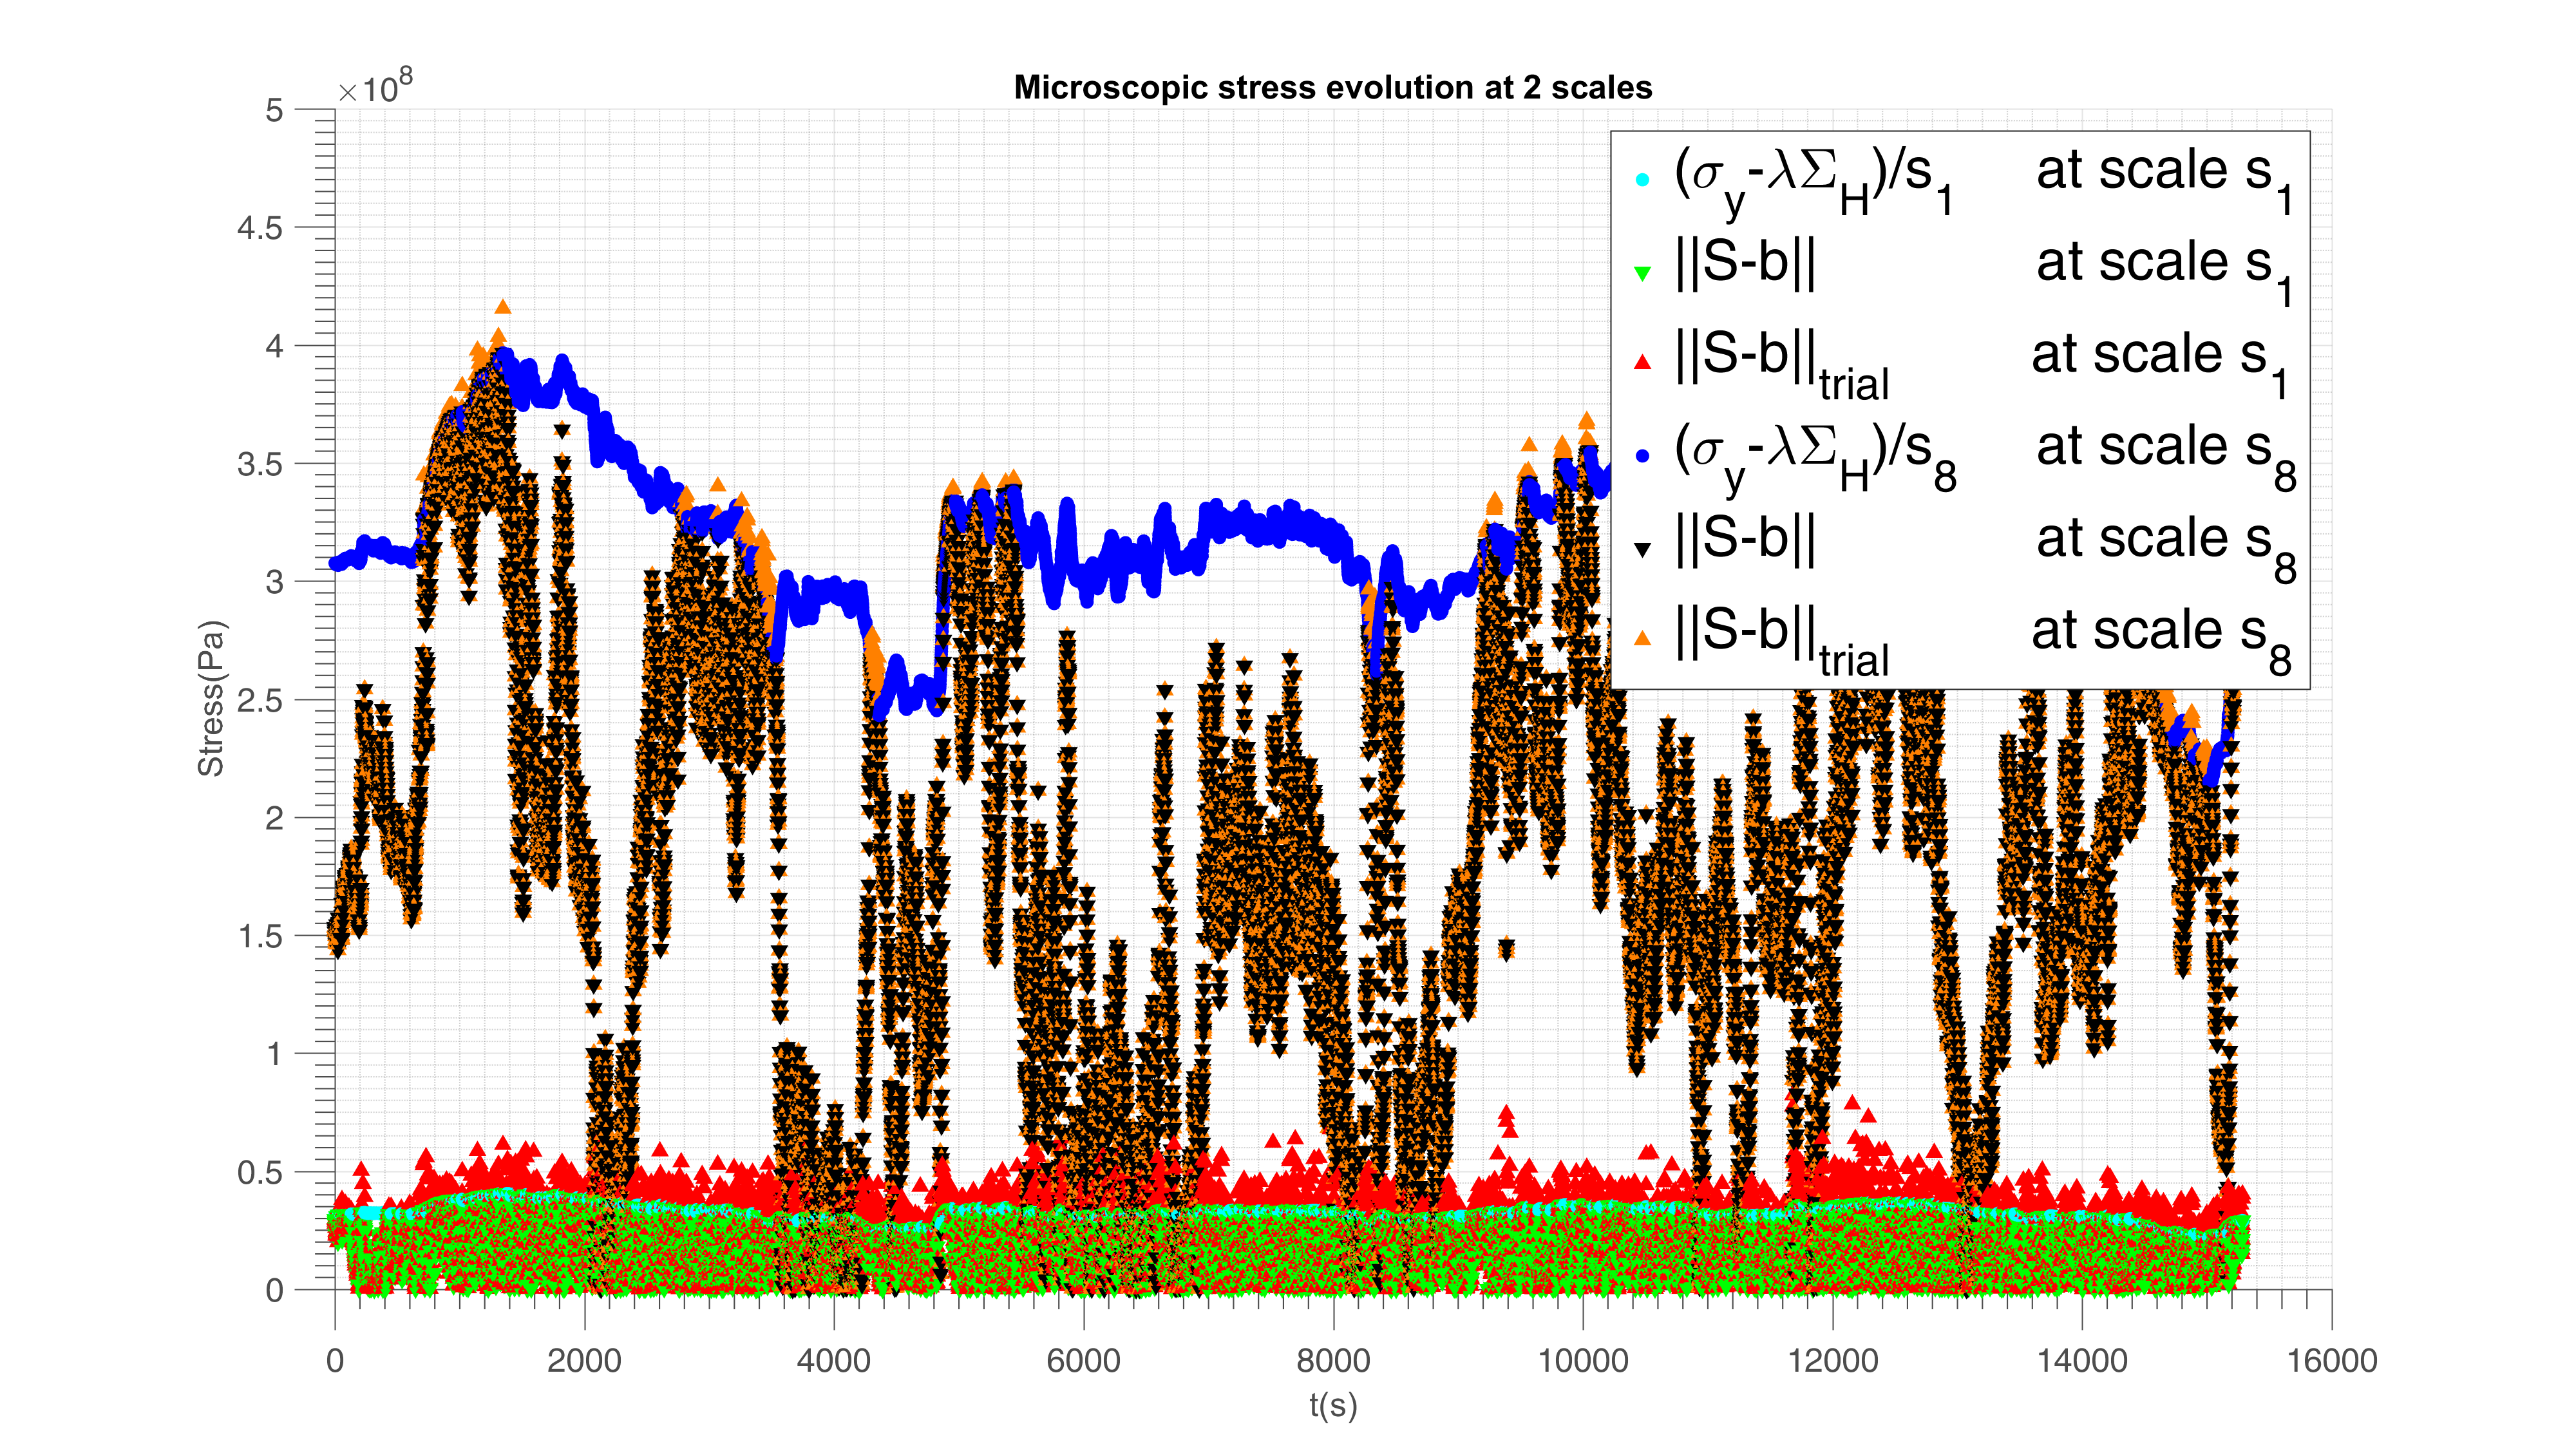
\includegraphics[width=\textwidth]{figures//trialreal1d1.png} 
	\caption{$\left\|  \uline{\uline{S}}-\uline{\uline{b}}\right\|_{trial}$ and $\left\|  \uline{\uline{S}}-\uline{\uline{b}}\right\|$ evolution with time under different weakening scales in PSA load history}
	\label{trialreal}
\end{figure}
\begin{figure}[!h]
	\centering
	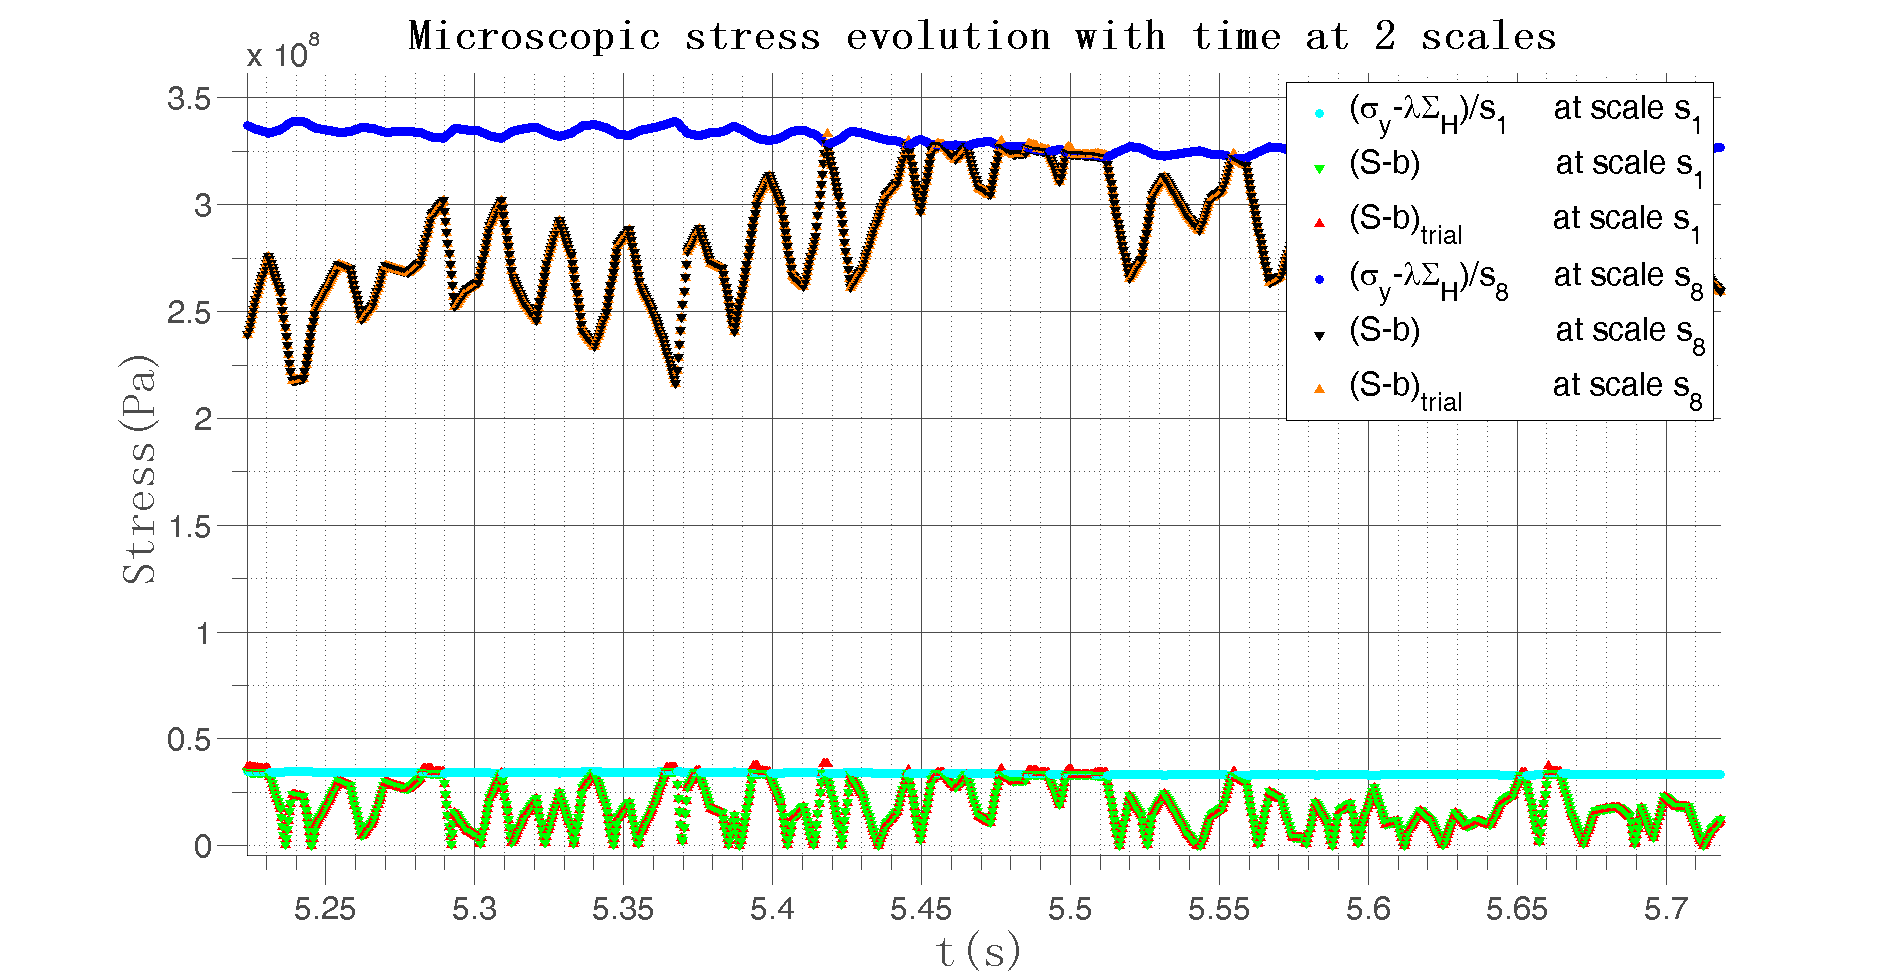
\includegraphics[width=\textwidth]{figures//trialreal1d2.png} 
	\caption{Circled area magnification in \figref{trialreal} where there is more $\left\|  \uline{\uline{S}}-\uline{\uline{b}}\right\|_{trial}>\sigma_y$(plasticity)  at $s_1$ than at $s_8$}
	\label{trialreal1d2}
\end{figure}
\begin{figure}[!h]
	\centering
	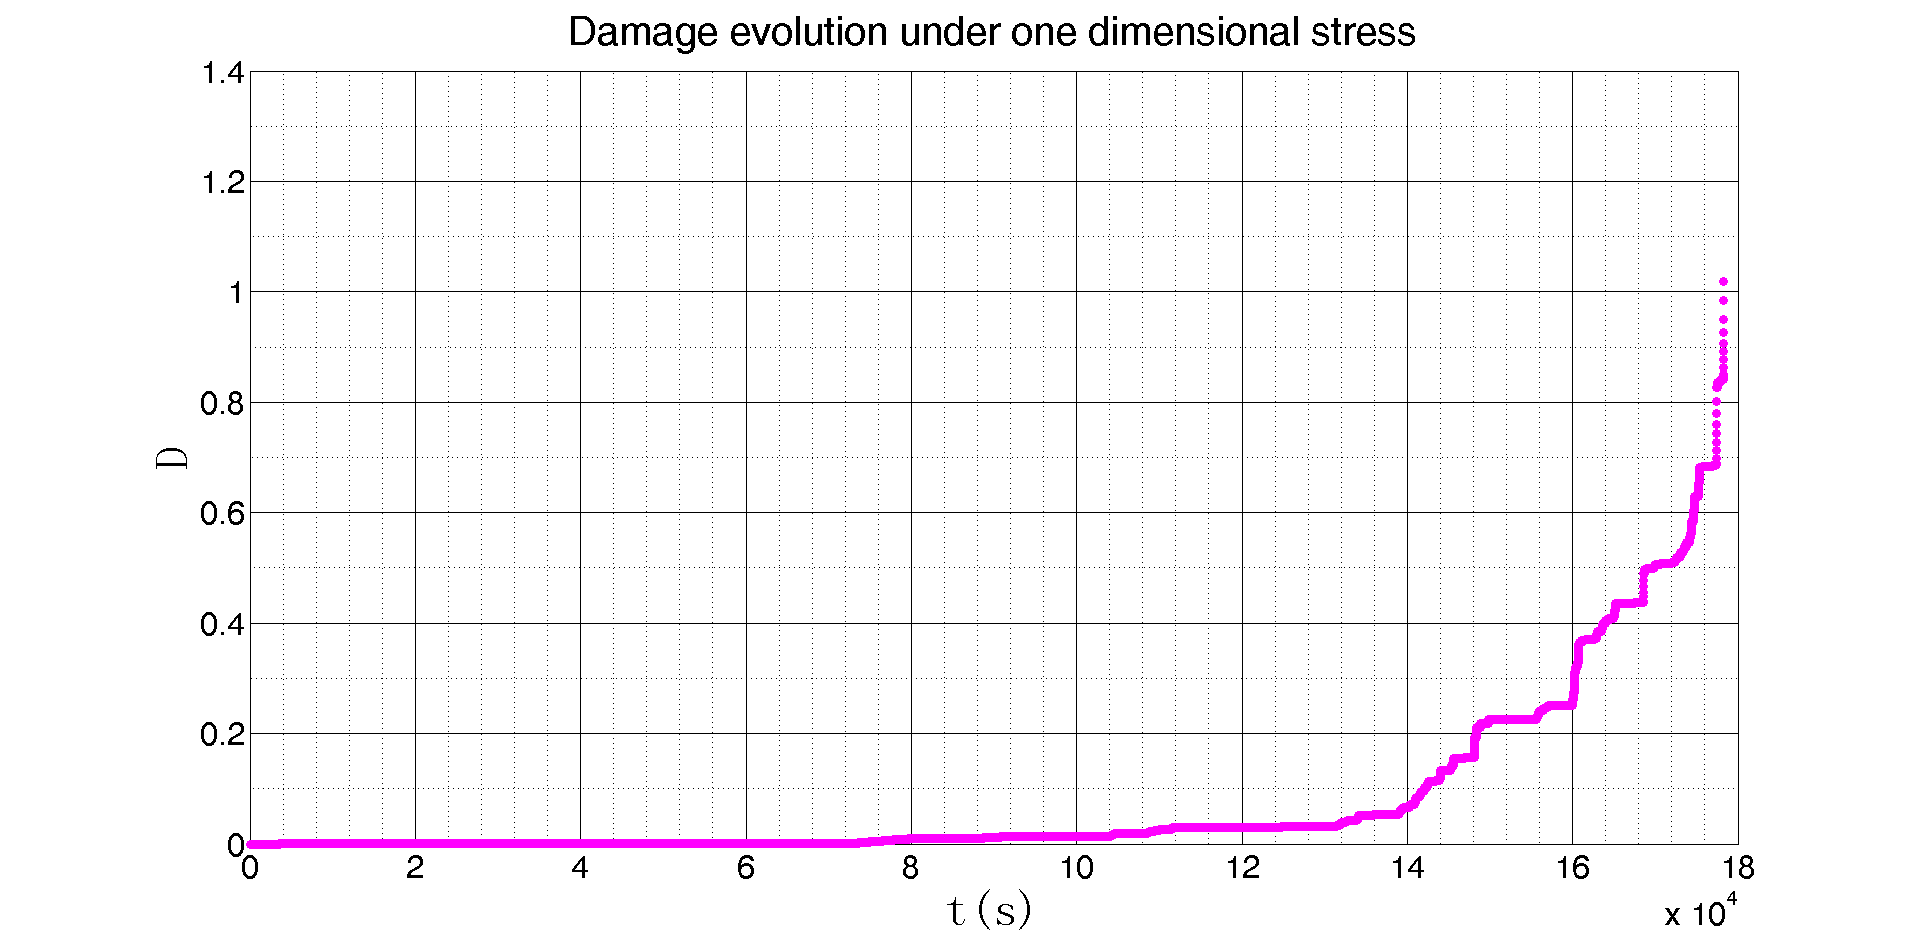
\includegraphics[width=\textwidth]{figures//damage1d.png} 
	\caption{Damage evolution with time at one dimension PSA load history}
	\label{damage1d}
\end{figure}

 \newpage
 \subsection{Multi-dimensional application to PSA data}
 We now consider a situation where we have force recorded measured in 3 different directions as shown in \figref{xyz}.
 \begin{figure}[!h]
 	\centering
 	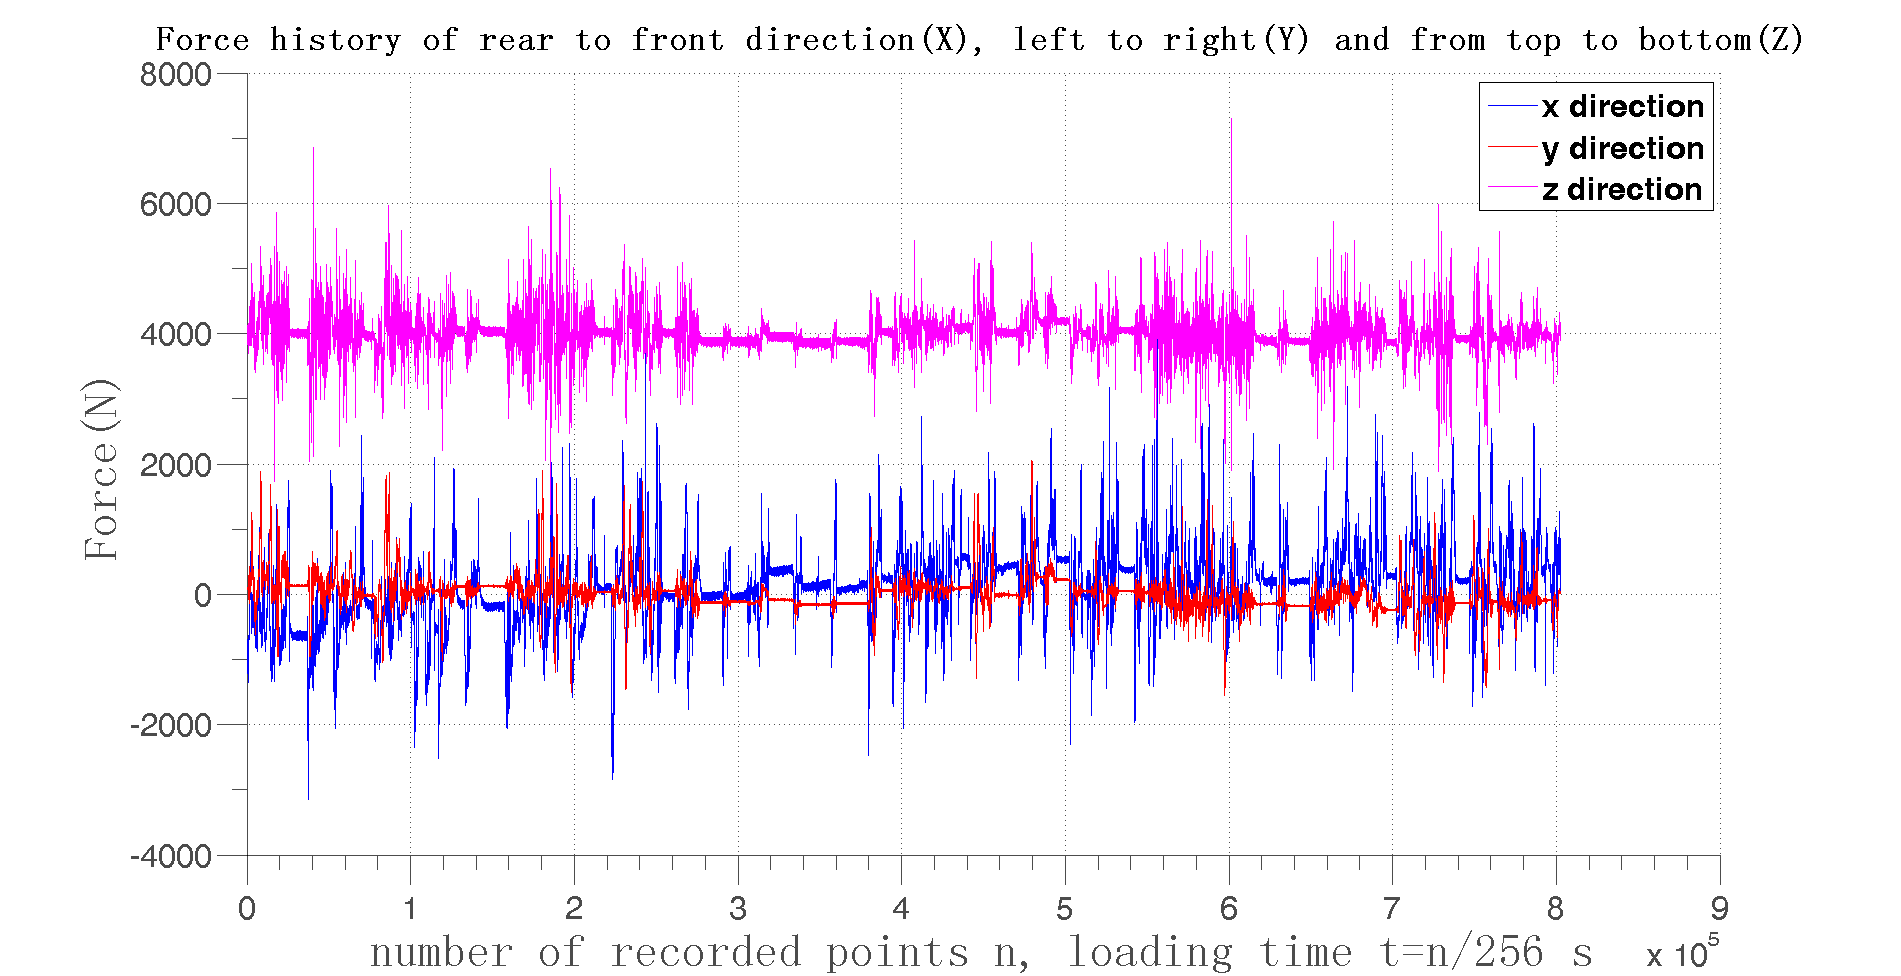
\includegraphics[width=\textwidth]{figures//xyz.png} 
 	\caption{Loading history of 3 different directions}
 	\label{xyz}
 \end{figure}
  \begin{figure}[!h]
  	\centering
  	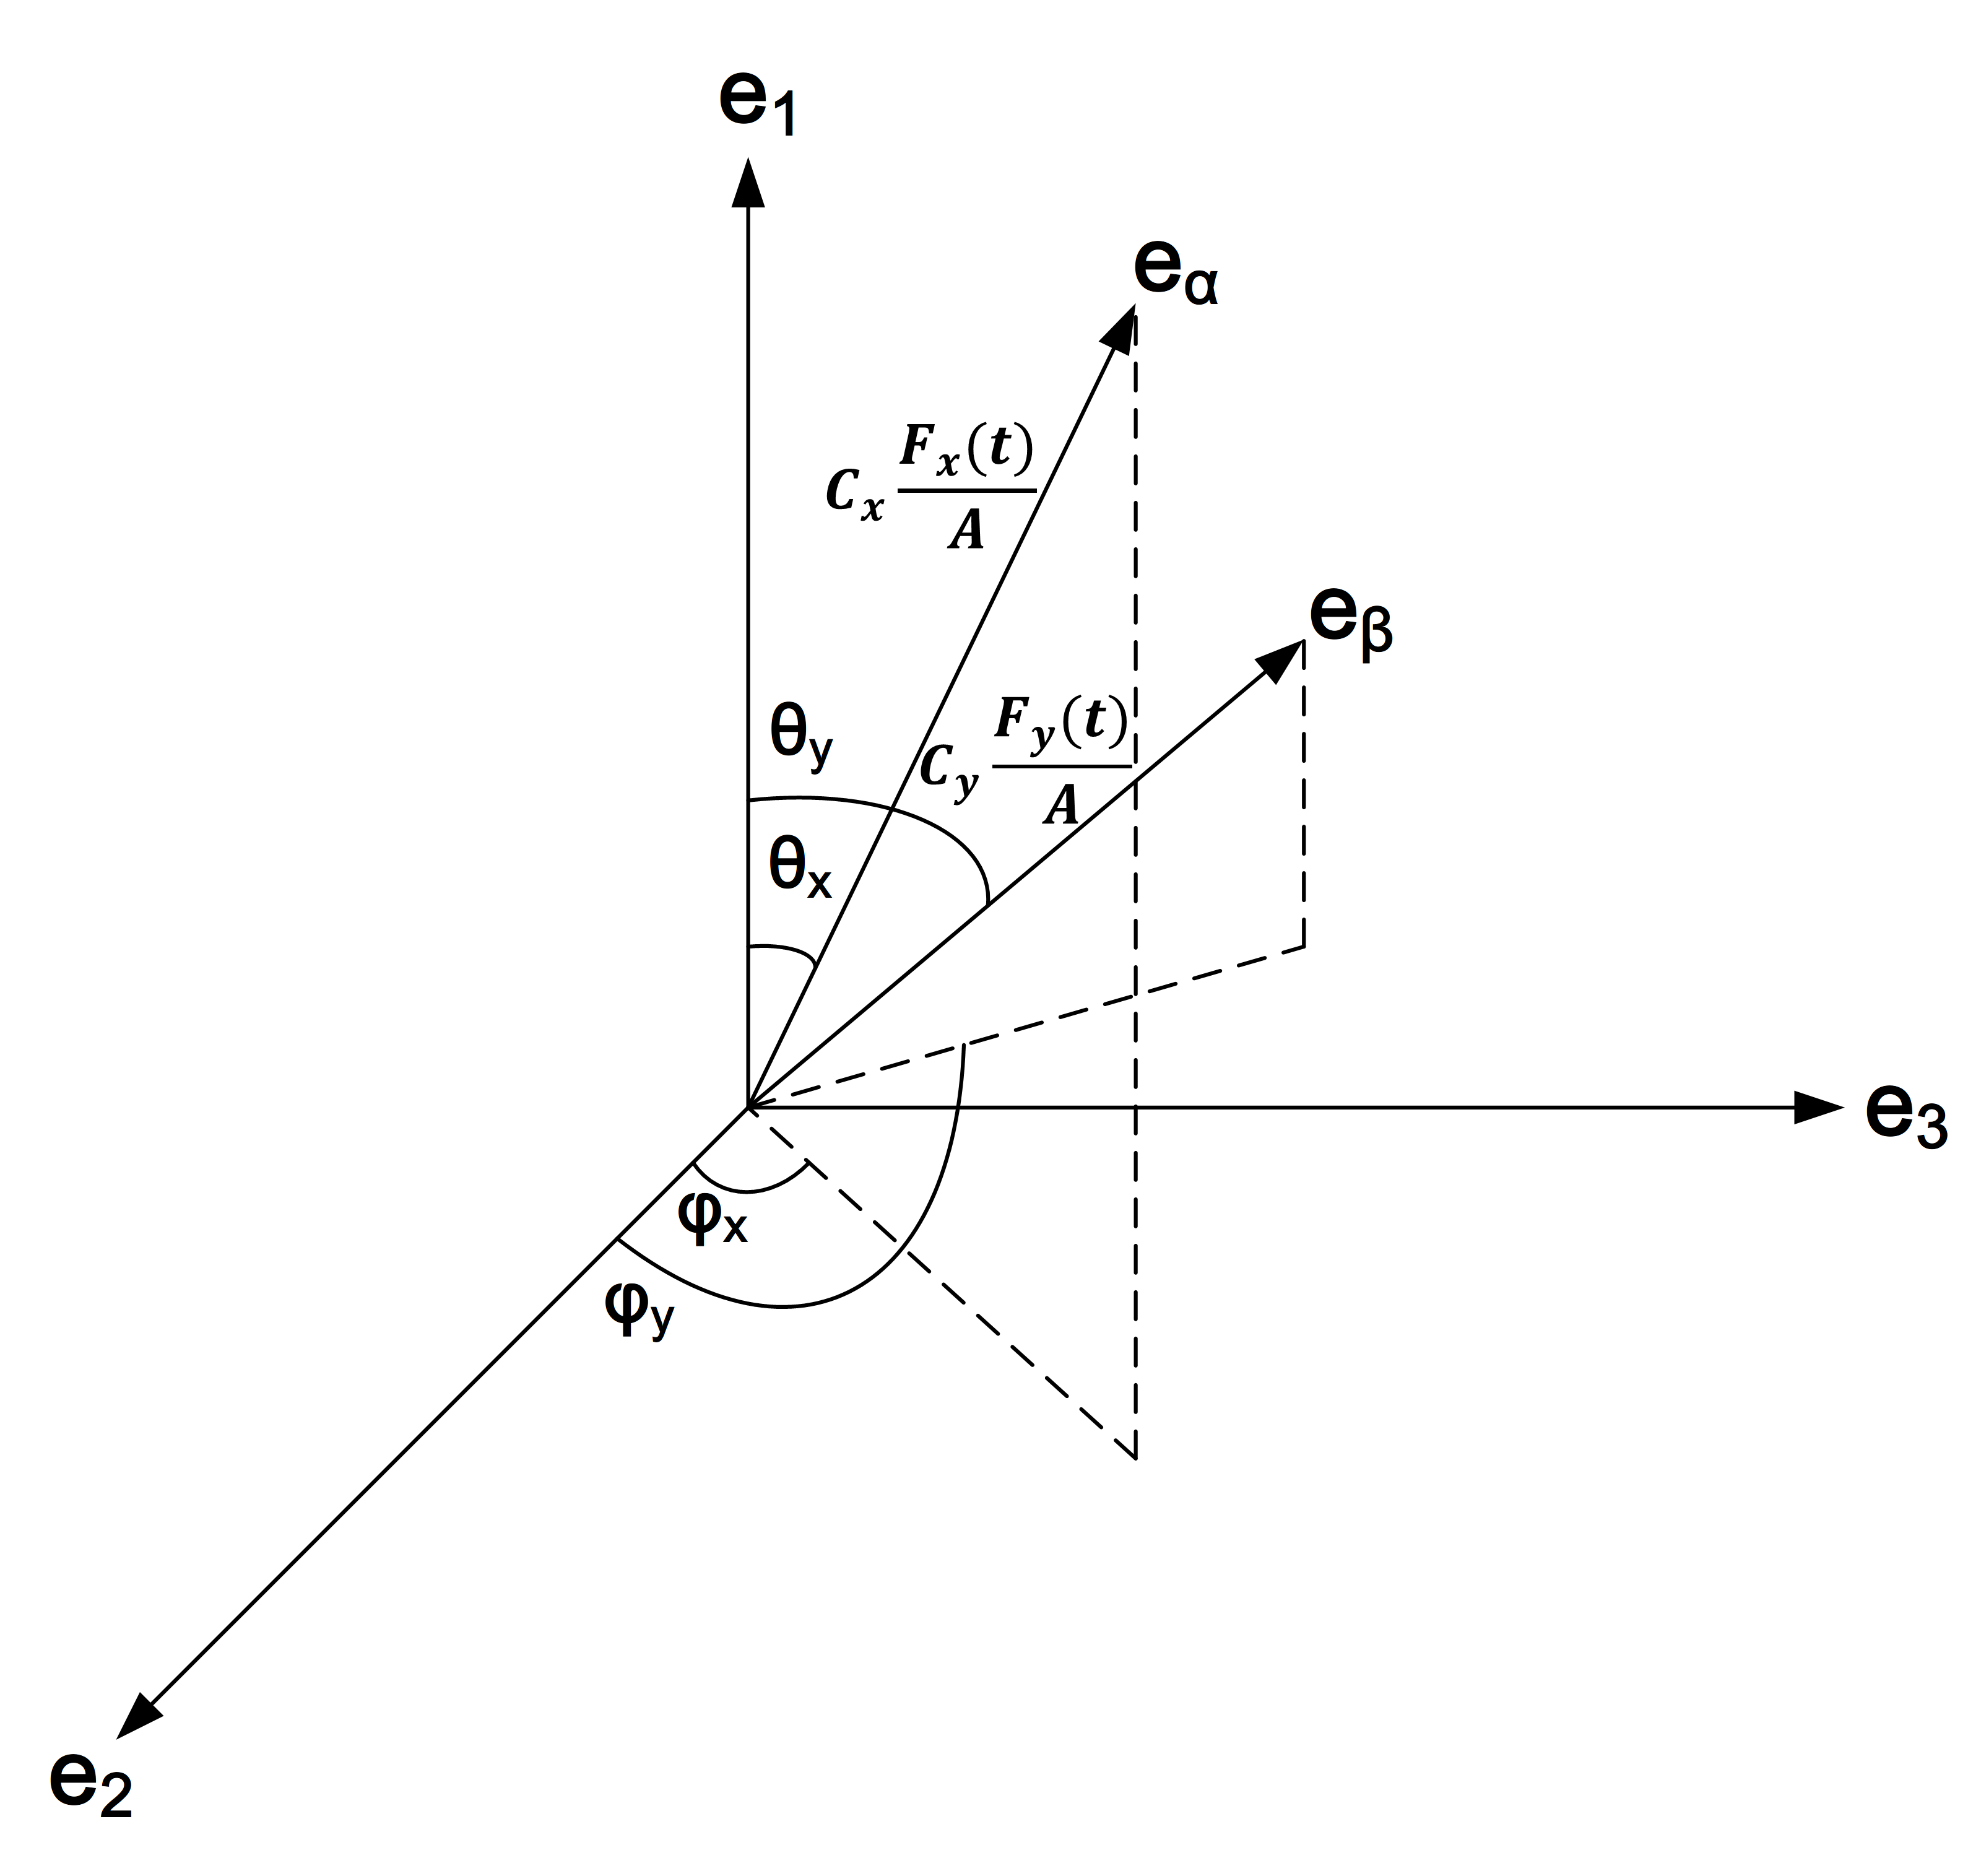
\includegraphics[width=0.7\textwidth]{figures//xab.png} 
  	\caption{Loading in 3 different directions}
  	\label{xab}
  \end{figure}
 In real case, the vertical force $F_z$ is much larger than the axial and horizontal forces $F_x$ and $F_y$, as shown in \figref{xyz}. However, in order to investigate large domains of interest, we first scale the axial and horizontal forces to reach comparable impact and transform them in principal stresses $c_x\dfrac{F_x}{A}$ applied along the stress principle vector $\uline{e}_\alpha$(respectively $\uline{e}_\beta$) that we choose randomly(\figref{xab}). We therefore consider the following macroscopic stress tensor:
 \begin{equation}
 \uline{\uline{\Sigma}}=\dfrac{F_z(t)}{A}\uline{e}_1\otimes \uline{e}_1+c_x\dfrac{F_x(t)}{A}\uline{e}_{\alpha}\otimes \uline{e}_{\alpha}+c_y\dfrac{F_y(t)}{A}\uline{e}_{\beta}\otimes \uline{e}_{\beta}
 \label{tensor1}
 \end{equation}
 where $\uline{e}_{\alpha}$  and $\uline{e}_{\beta}$ are principal vectors whose spherical coordinate are $\theta_x$, $\varphi_x$,  $\theta_y$ and $\varphi_y$ respectively:
  $$\uline{e}_{\alpha}=cos\theta_x\uline{e}_1+sin\theta_xcos\varphi_x\uline{e}_2+sin\theta_xsin\varphi_x\uline{e}_3,$$
 $$\uline{e}_{\beta}=cos\theta_y\uline{e}_1+sin\theta_ycos\varphi_y\uline{e}_2+sin\theta_ysin\varphi_y\uline{e}_3.$$
 Here $F_x(t)$, $F_y(t)$, $F_z(t)$ are from test data, and $\theta_x$, $\varphi_x$, $\theta_y$, $\varphi_y$ are structural parameters to be chosen randomly.The physical data are the same with parameters in Table.\ref{Sin}. The structural data we choose is shown in Table.\ref{structural}.
 
  \begin{table}[!h]
  	\centering
    \begin{tabular}{rrrrrrrr}
  		\hline
  		\textbf{Parameter} & A($m^2$) & $c_x$ & $c_y$ & $\theta_x$ & $\varphi_x$ & $\theta_y$ & $\varphi_y$ \\
  		\textbf{Value}      & 1/6e4                  & 10    & 60    & 0.5        & 0.3         & 0.6        & 0.4         \\ \hline
  	\end{tabular}
  	\caption{The structural data in 3D analysis}
  	\label{structural}
  \end{table}
 
 The underlying assumption is that a unit load on wheel in direction $\uline{e}_x$ creates a stress tensor at point $M$ given by:
 $$c_x\dfrac{F_x(t)}{A}\uline{e}_{\alpha}\otimes \uline{e}_{\alpha},$$
 where $\uline{e}_{\alpha}\otimes \uline{e}_{\alpha}$ defines the local structural response of the vehicle.
 
 Replacing $\uline{e}_{\alpha}$ and $\uline{e}_{\beta}$ in Eq.\eqref{tensor1} we get the stress tensor in Eq.\eqref{tensor2} in the annex. 
 


 
 
 The plot of $\left\|  \uline{\uline{S}}-\uline{\uline{b}}\right\|_{trial}$ and $\left\|  \uline{\uline{S}}-\uline{\uline{b}}\right\|$ under 2 different scales are shown in \figref{trialreal3d}.
\begin{figure}[!h]
	\centering
	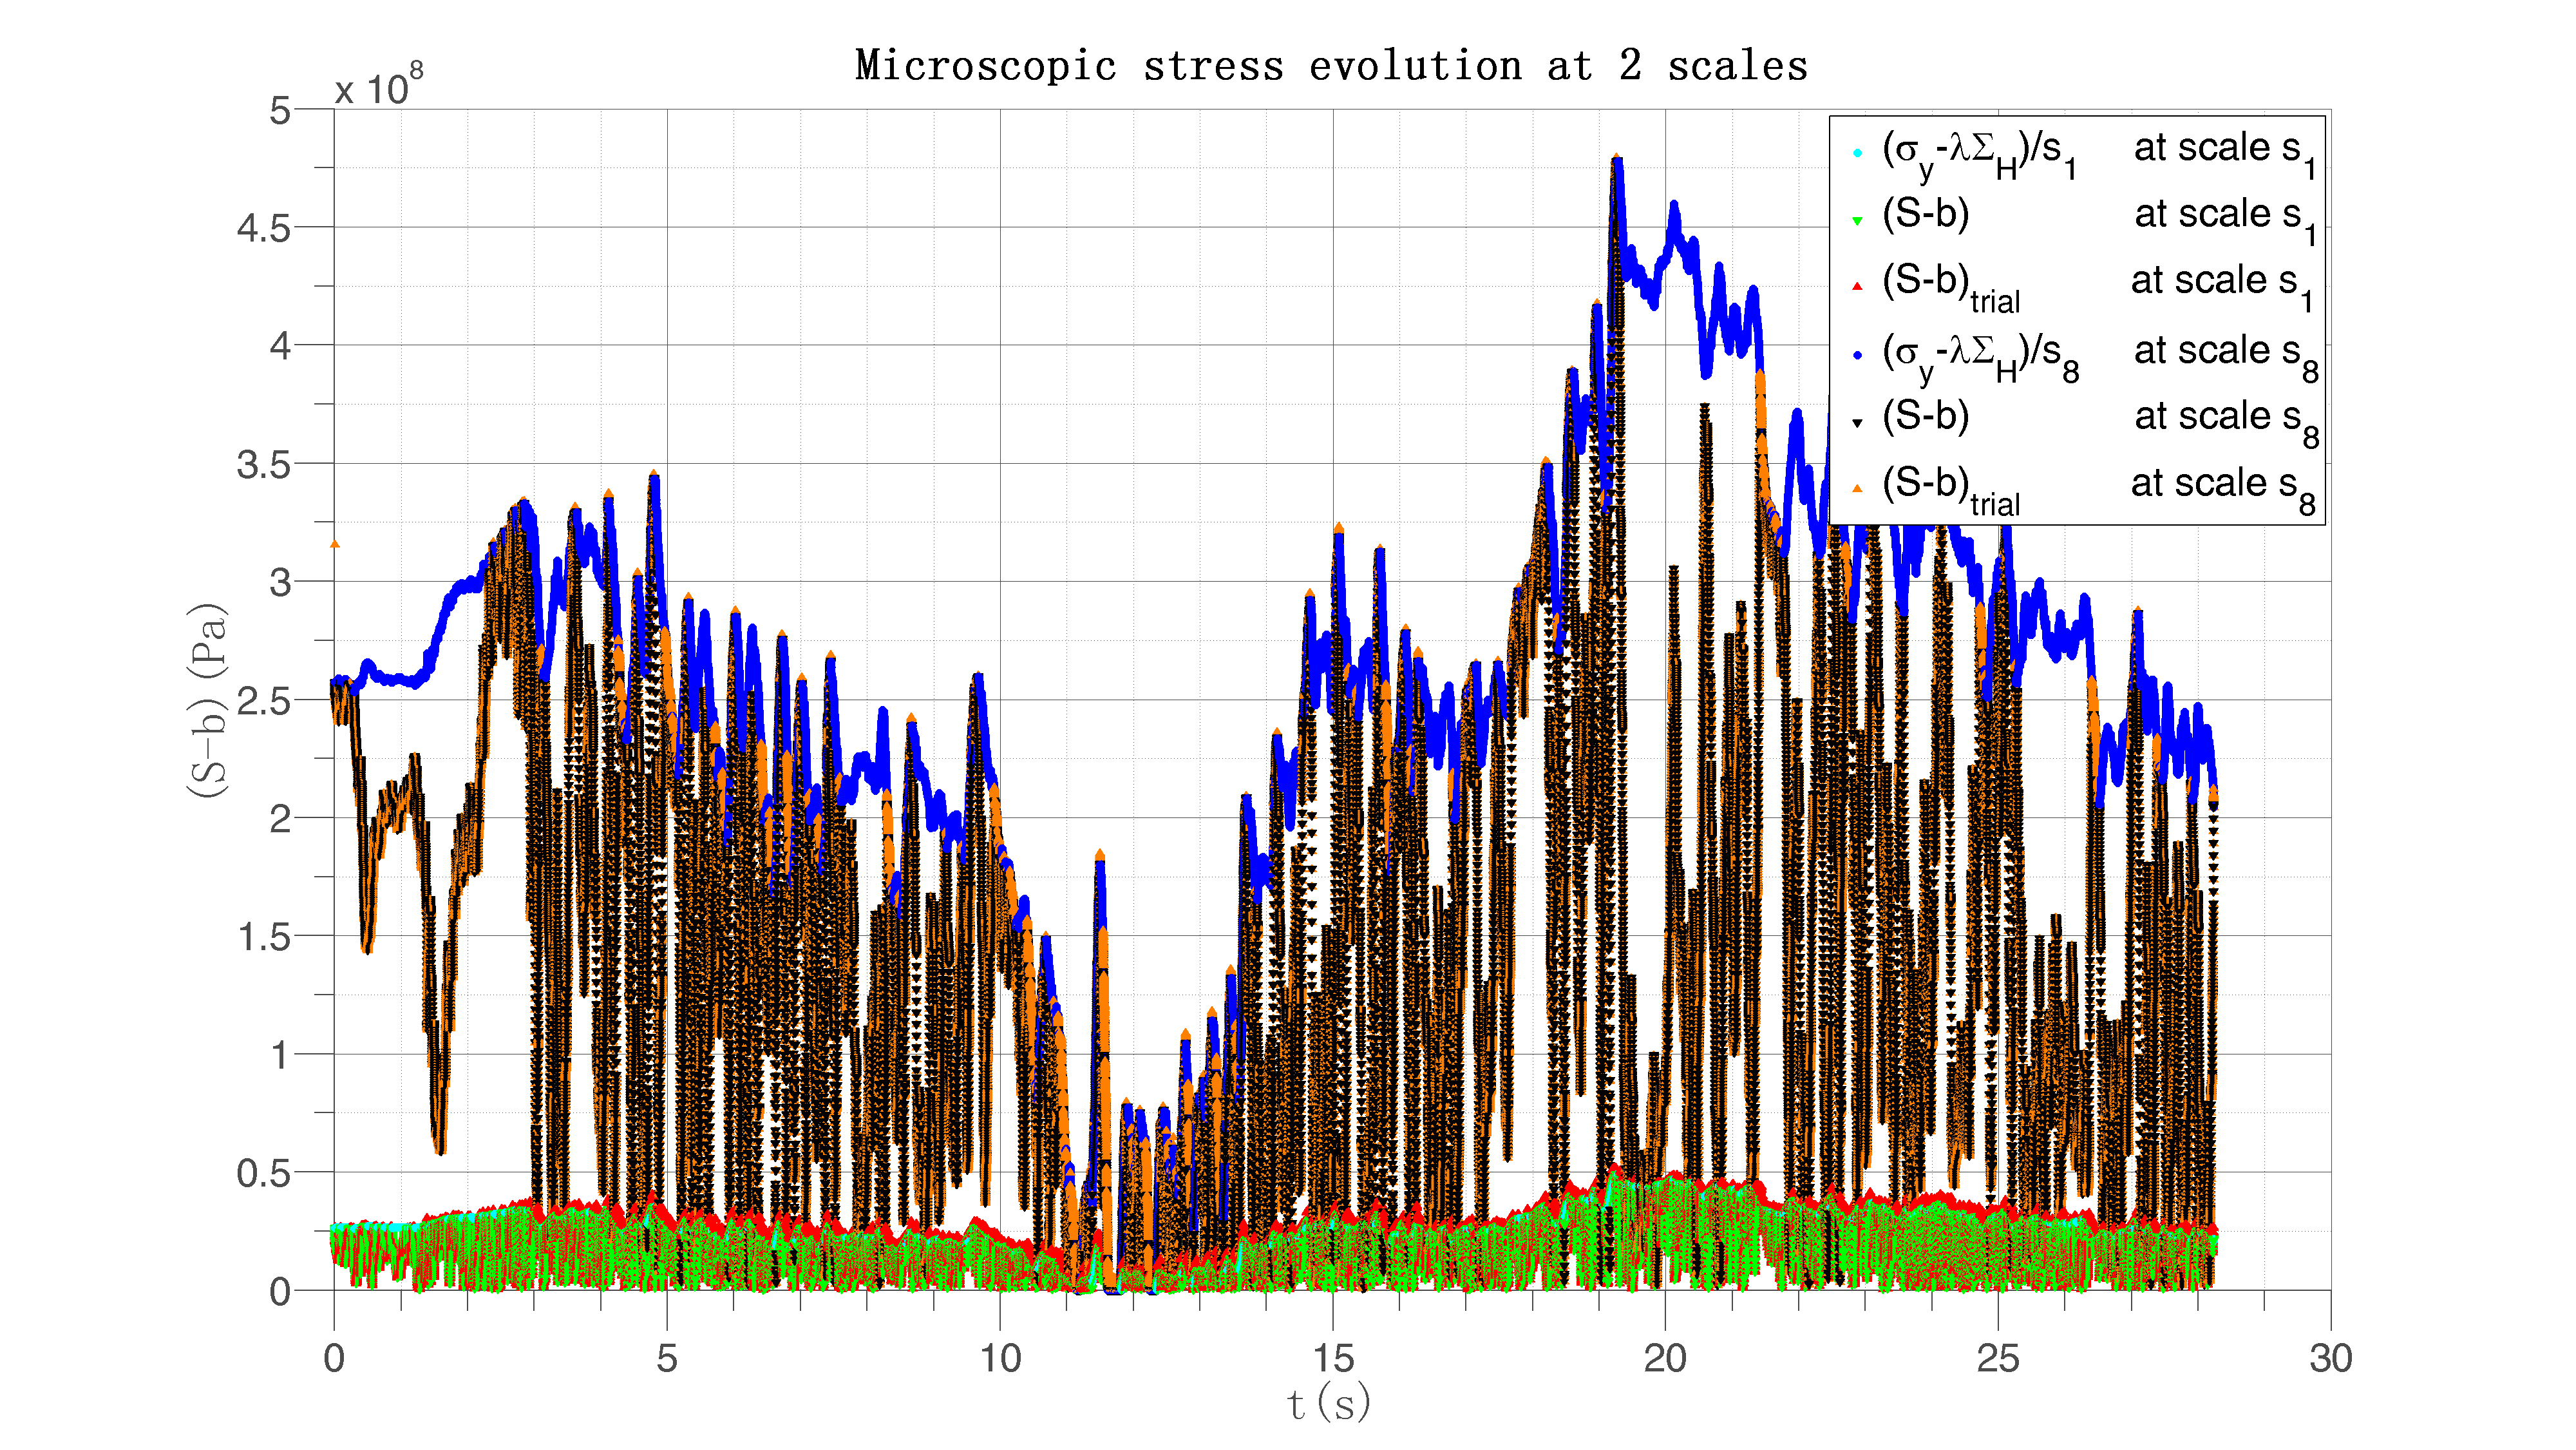
\includegraphics[width=\textwidth]{figures//trialreal3d.png} 
	\caption{$\left\|  \uline{\uline{S}}-\uline{\uline{b}}\right\|_{trial}$ and $\left\|  \uline{\uline{S}}-\uline{\uline{b}}\right\|$ evolution with time under different weakening scales in PSA load history}
	\label{trialreal3d}
\end{figure} 



In the load history, when $\left\|  \uline{\uline{S}}-\uline{\uline{b}}\right\|_{trial}>\sigma_y$, the damage accumulates. However, under scale $s_{8}$, there are much less damage accumulation than under scale $s_1$.  In this way we do not neglect the small influences in load history and the big fluctuation in stress is magnified which reflects the real situation. 

%\iffalse
The damage evolves like in \figref{dam3d}. 


\begin{figure}[!h]
	\centering
	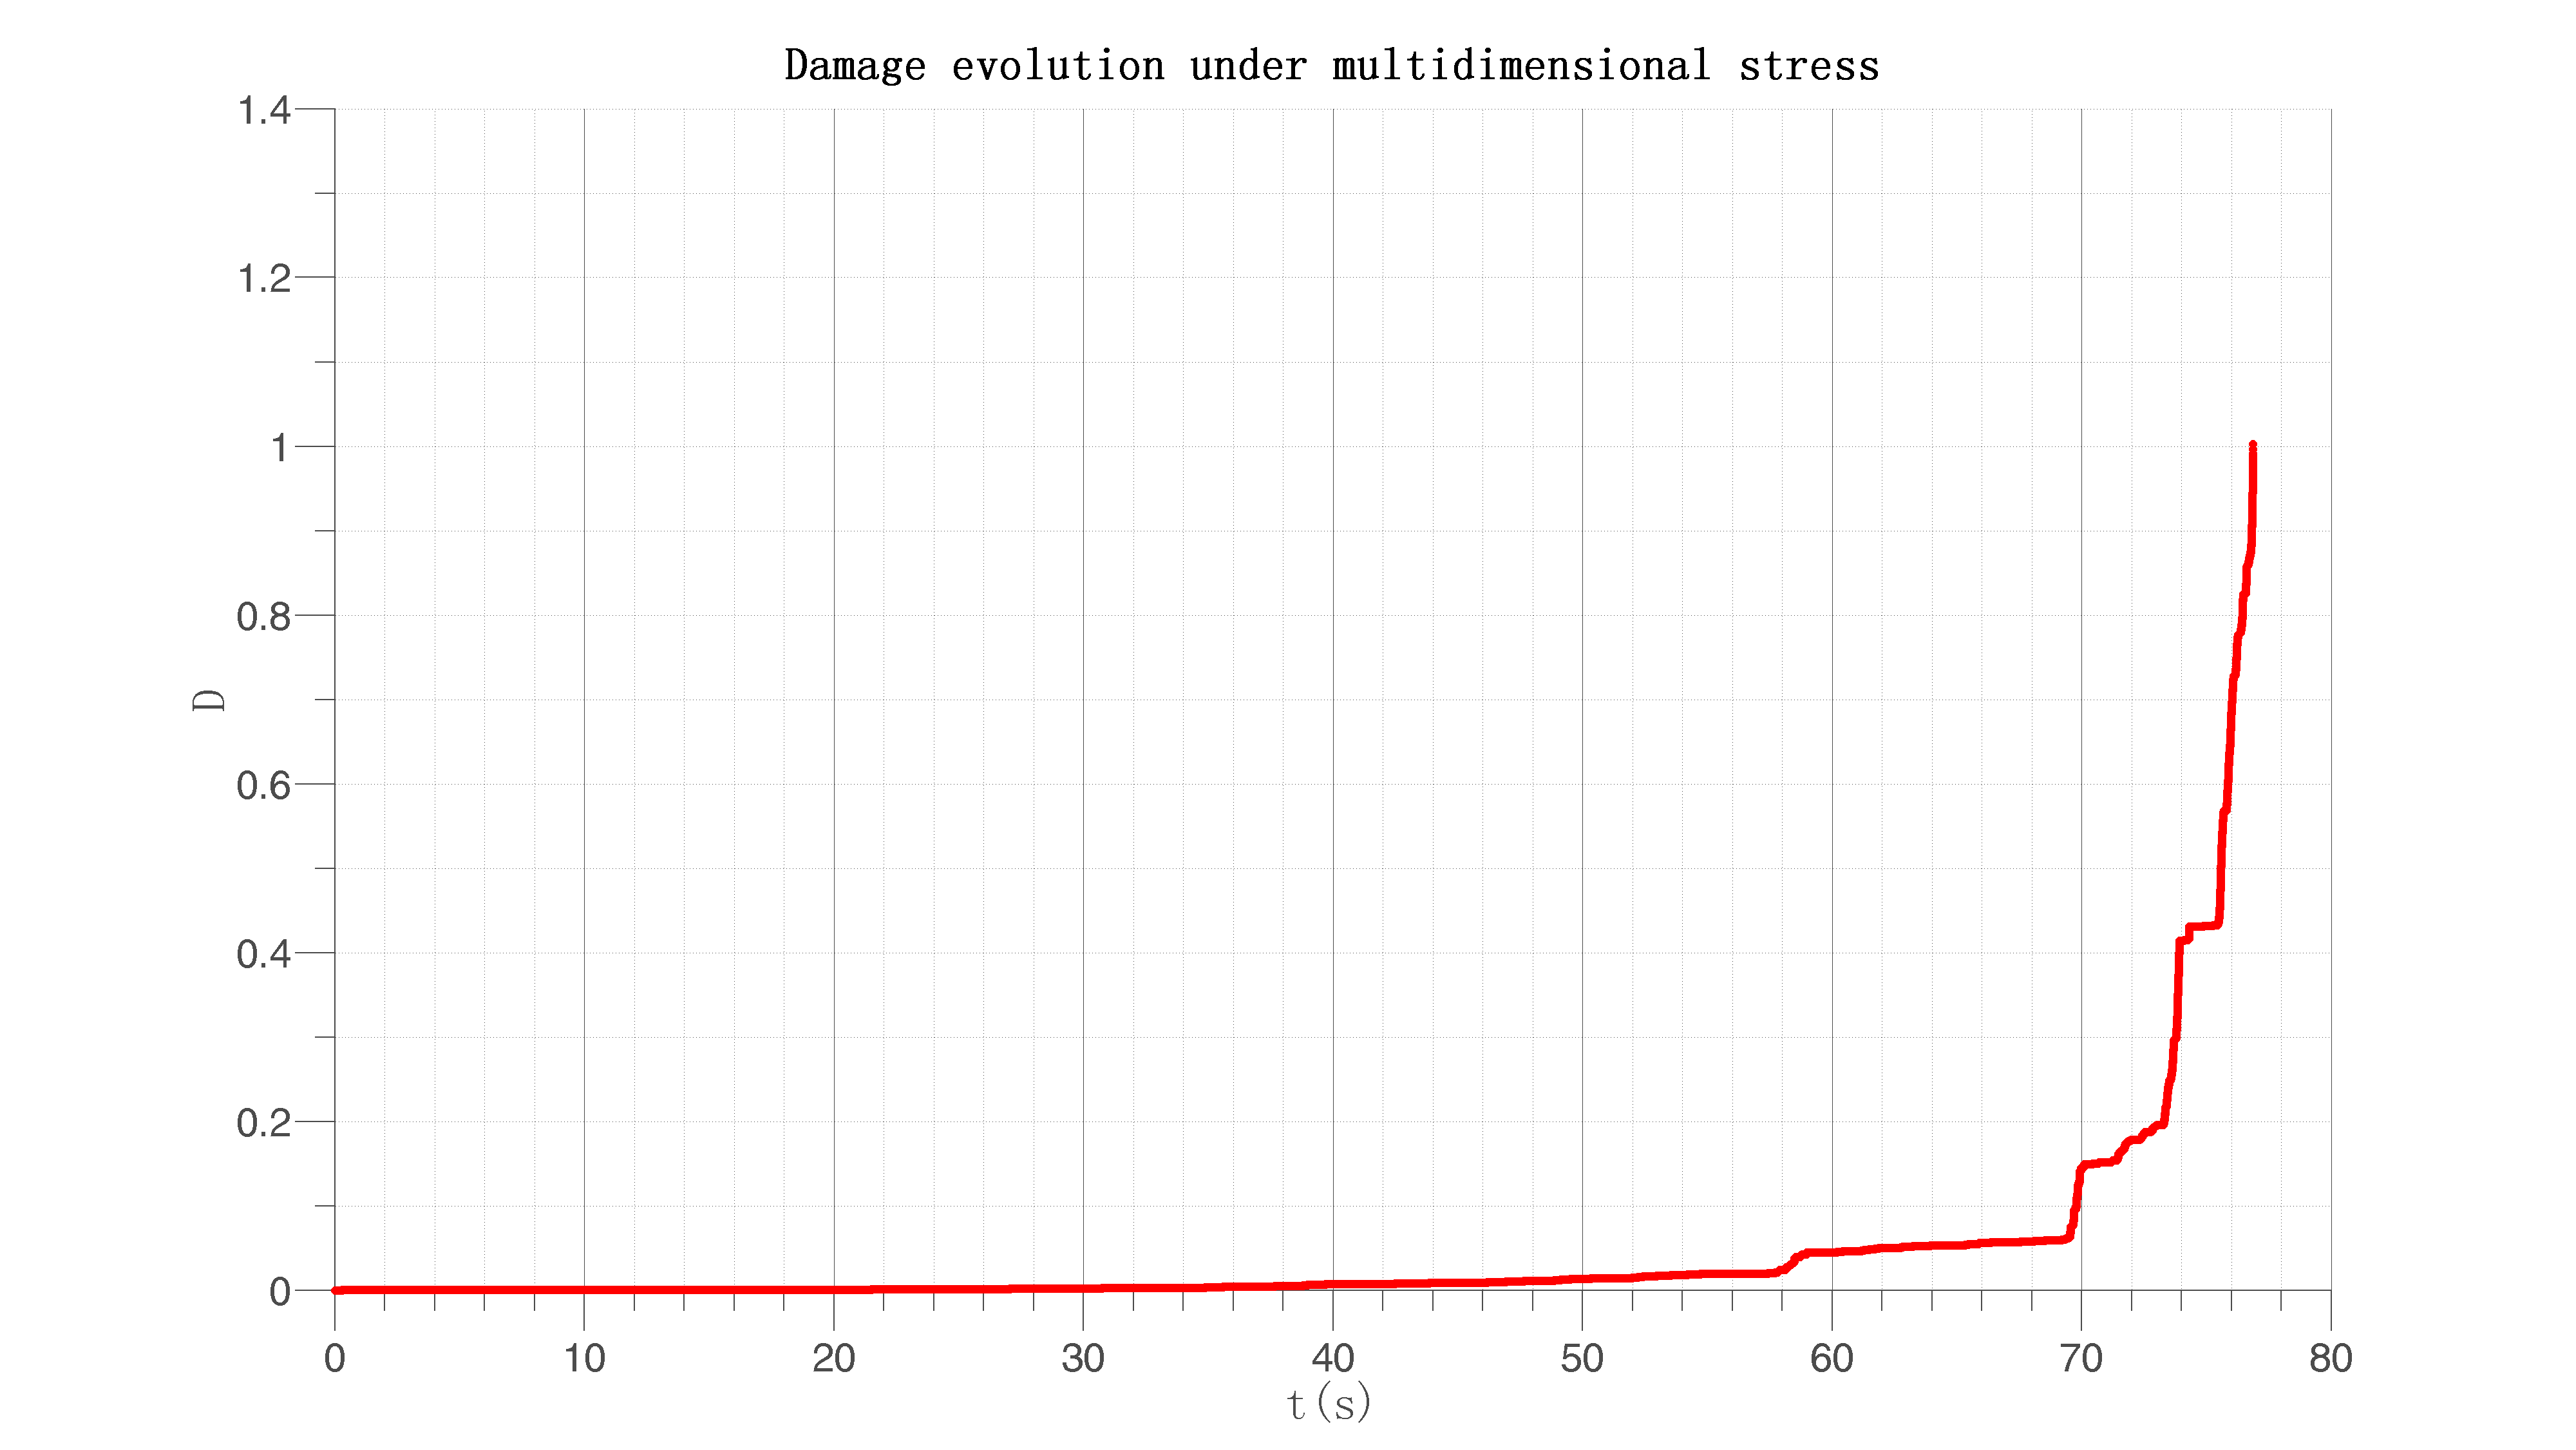
\includegraphics[width=\textwidth]{figures//damage3d.png} 
	\caption{Damage evolution under multidimensional stress}
	\label{dam3d}
\end{figure}
%\fi

We can improve the result by inserting more arithmetic sequence points between every 2 recorded points. As is shown in Table.\ref{steppoints} :

\begin{table}[!h]
	\centering
	\caption{Arithmetic sequence points density effect}
	\label{steppoints}
\begin{tabular}{cc}
	\hline
	\textbf{Arithmetic sequence points between every two points} & \textbf{Total time to failure(s)} \\ \hline
	10                                                           & 78.63711                          \\ 
	20                                                           & 72.24630                          \\ 
	30                                                           & 70.25793                          \\ 
	50                                                           & 68.69148                          \\ 
	100                                                          & 67.49223                          \\ \hline
\end{tabular}
\end{table}

 
 
\clearpage
\section{Discussion}
We work on the stress tensor directly in 3D analysis in stead of using the multidimensional equivalent stress.
The strategy can be made more complex by introducing a local space averaging process in the calculation of the local damage, and by taking more general plastic flows. The energy based fatigue approach takes into account impurities and hardness in the material and is applicable to any type of micro plasticity law and multiaxial load geometry. The small step-by-step strategy does not ignore small fluctuations in the load history. 

Further research of energy based failure criteria should be focused on the following aspects:
\begin{enumerate}
\item The  accommodation law might be more elaborate than kinematic hardening.

\vspace{6pt}
\item The differentiation of shear stress and normal stress effect on fatigue life should be clarified.

\vspace{6pt}
\item The non-linearity parameter $\alpha$ contains the stress $\sigma$, so it can evolve with time. But for complex loading history, should it change at every time step?

\end{enumerate}

\vspace{6pt}
\noindent
\textbf{Acknowledgments}

\vspace{6pt}
We are grateful for the financial and technical support of Chaire PSA.

\bibliographystyle{unsrt}
\bibliography{11}
\addcontentsline{toc}{section}{Reference}

\clearpage
\appendix
\appendixpage
\addcontentsline{toc}{section}{Appendices}\markboth{APPENDICES}{}
\lstset{% general command to set parameter(s)
	basicstyle=\small, % 设置字体大小
	keywordstyle=\color{red}, % 设置关键字格式(颜色等等)
	identifierstyle=, % nothing happens
	commentstyle=\color{blue}, % 设置注释的格式
	stringstyle=\ttfamily, % typewriter type for strings
	showstringspaces=false} % no special string spaces
\begin{subappendices}
	\section{DETAILED EXPLOITATION}
	************************************************************************************

 A DETAILED DESCRIPTION OF ANALYTICAL EXPLOITATION ON UNIAXIAL CYCLE
 
\noindent              
************************************************************************************

\noindent
\textbf{Phase 1:} The deviatoric stress amplitude increases from $\sigma_y/s$ to $S_{max}$.

\noindent
The material is in local plastic regime, then $\dot{\varepsilon}^p>0$ and $\dot{\sigma}-\dot{b}=0$ $\Rightarrow$ $\dot{\Sigma}-\dfrac{E}{1+\nu}\dot{\varepsilon}^p=\dfrac{kE}{E-k}\dot{\varepsilon}^p$ $\Rightarrow$ 
$$\dot{\varepsilon}^p=\dfrac{(E- k)(1+\nu)}{E(E+k\nu)}\dot{\Sigma}.$$

\vspace{6pt}
\noindent
$\Rightarrow$ $\dot{\varepsilon}^p$ varies from 0 to $\dfrac{(E- k)(1+\nu)(S_{max}-\sigma_y/s)}{E(E+k\nu)}$.

\vspace{6pt}
\noindent
From Taylor-Lin scale transition model:
$$\dot{\sigma}=\dot{\Sigma}-\dfrac{E}{1+\nu}\dot{\varepsilon}_p=\dot{\Sigma}-\dfrac{E-k}{E-\nu k}\dot{\Sigma}=\dfrac{k(1-\nu)}{E-k\nu}\dot{\Sigma}.$$

\vspace{6pt}
\noindent
$\Rightarrow$ $\sigma$ varies from $\sigma_y/s$ to $\sigma_y/s+\dfrac{k(1-\nu)(S_{max}-\sigma_y/s)}{E-k\nu}$.

\vspace{6pt}
$$\dot{b}=\dot{\Sigma}-\dfrac{E}{1+\nu}\dot{\varepsilon}_p=\dot{\Sigma}-\dfrac{E-k}{E-\nu k}\dot{\Sigma}=\dfrac{k(1-\nu)}{E-k\nu}\dot{\Sigma}.$$

\vspace{6pt}
\noindent
$\Rightarrow$ $b$ varies from $0$ to $\dfrac{k(1-\nu)(S_{max}-\sigma_y/s)}{E-k\nu}$.

\vspace{6pt}
\noindent
So the energy dissipation rate is: $$(\sigma-b)\dot{\varepsilon}^p=\dfrac{\sigma_y}{s}\dot{\varepsilon}^p=\dfrac{\sigma_y}{s}\dfrac{(E- k)(1+\nu)}{E(E+k\nu)}\dot{\Sigma}.$$

\noindent
The energy dissipation is: $$(\sigma-b)\Delta\varepsilon^p=\dfrac{\sigma_y}{s}\dfrac{(E- k)(1+\nu)(S_{max}-\sigma_y/s)}{E(E+k\nu)}.$$

\vspace{6pt}
\noindent
\textbf{Phase 2:} The deviatoric stress amplitude decreases from $S_{max}$ to $S_{max}-2\sigma_y/s$.

\noindent
The material is in local elastic regime, then $\dot{\varepsilon}^p=0$ and $\dot{\sigma}-\dot{b}=0$ $\Rightarrow$

\vspace{6pt}
\noindent
$\dot{b}=0$, $\dot{\sigma}=\dot{\Sigma}-\dfrac{E}{1+\nu}\dot{\varepsilon}_p=\dot{\Sigma}$.

\vspace{6pt}
\noindent
$\sigma$ varies from $\sigma_y/s+\dfrac{k(1-\nu)(S_{max}-\sigma_y/s)}{E-k\nu}$ to $-\sigma_y/s+\dfrac{k(1-\nu)(S_{max}-\sigma_y/s)}{E-k\nu}$.

\vspace{6pt}
\noindent
$\sigma-b$ varies from $\sigma_y/s$ to $-\sigma_y/s$.

\vspace{6pt}
\noindent
The energy dissipation rate is: $$(\sigma-b)\dot{\varepsilon}^p=0.$$

\vspace{6pt}
\noindent
\textbf{Phase 3:} The deviatoric stress amplitude decreases from $S_{max}-2\sigma_y/s$ to $-S_{max}$.

\noindent
The material is in local plastic regime, then $\dot{\varepsilon}^p>0$ and $\dot{\sigma}-\dot{b}=0$ $\Rightarrow$ 
$$\dot{\varepsilon}^p=\dfrac{(E- k)(1+\nu)}{E(E+k\nu)}\dot{\Sigma}$$ as opposite to phase 1 for $\dot{\Sigma}<0$.

\vspace{6pt}
\noindent
$\Rightarrow$ $\varepsilon^p$ varies from $\dfrac{(E- k)(1+\nu)(S_{max}-\sigma_y/s)}{E(E+k\nu)}$ to 

\noindent
$\dfrac{(E- k)(1+\nu)(S_{max}-\sigma_y/s-S_{max}-(S_{max}-2\sigma_y/s))}{E(E+k\nu)}=-\dfrac{(E- k)(1+\nu)(S_{max}-\sigma_y/s)}{E(E+k\nu)}$.

\vspace{6pt}
\noindent
From Taylor-Lin scale transition model:
$$\dot{\sigma}=\dot{\Sigma}-\dfrac{E}{1+\nu}\dot{\varepsilon}_p=\dot{\Sigma}-\dfrac{E-k}{E-\nu k}\dot{\Sigma}=\dfrac{k(1-\nu)}{E-k\nu}\dot{\Sigma}.$$

\vspace{6pt}
\noindent
$\Rightarrow$ $\sigma$ varies from $-\sigma_y/s+\dfrac{k(1-\nu)(S_{max}-\sigma_y/s)}{E-k\nu}$ to $-\sigma_y/s-\dfrac{k(1-\nu)(S_{max}-\sigma_y/s)}{E-k\nu}$.

\vspace{6pt}
$$\dot{b}=\dot{\Sigma}-\dfrac{E}{1+\nu}\dot{\varepsilon}_p=\dot{\Sigma}-\dfrac{E-k}{E-\nu k}\dot{\Sigma}=\dfrac{k(1-\nu)}{E-k\nu}\dot{\Sigma}.$$
\vspace{6pt}
\noindent
$\Rightarrow$ $b$ varies from $\dfrac{k(1-\nu)(S_{max}-\sigma_y/s)}{E-k\nu}$ to $-\dfrac{k(1-\nu)(S_{max}-\sigma_y/s)}{E-k\nu}$.

\vspace{6pt}
\noindent
So the energy dissipation rate is: $$(\sigma-b)\dot{\varepsilon}^p=-\dfrac{\sigma_y}{s}\dot{\varepsilon}^p=-\dfrac{\sigma_y}{s}\dfrac{(E- k)(1+\nu)}{E(E+k\nu)}\dot{\Sigma}.$$

\noindent
The energy dissipation is: $$(\sigma-b)\Delta\varepsilon^p=-\dfrac{\sigma_y}{s}\dfrac{(E- k)(1+\nu)(-2S_{max}+2\sigma_y/s)}{E(E+k\nu)}=\dfrac{2\sigma_y}{s}\dfrac{(E- k)(1+\nu)(S_{max}-\sigma_y/s)}{E(E+k\nu)}.$$



\vspace{6pt}
\noindent
\textbf{Phase 4:} The deviatoric stress amplitude increases from $-S_{max}$ to $-S_{max}+2\sigma_y/s$.

\noindent
The material is in local elastic regime, then $\dot{\varepsilon}^p=0$ and $\dot{\sigma}-\dot{b}=0$ $\Rightarrow$

\vspace{6pt}
\noindent
$\dot{b}=0$, $\dot{\sigma}=\dot{\Sigma}-\dfrac{E}{1+\nu}\dot{\varepsilon}_p=\dot{\Sigma}$.

\vspace{6pt}
\noindent
$\sigma$ varies from $-\sigma_y/s-\dfrac{k(1-\nu)(S_{max}-\sigma_y/s)}{E-k\nu}$ to $\sigma_y/s-\dfrac{k(1-\nu)(S_{max}-\sigma_y/s)}{E-k\nu}$.

\vspace{6pt}
\noindent
$\sigma-b$ varies from $-\sigma_y/s$ to $\sigma_y/s$.

\vspace{6pt}
\noindent
So the energy dissipation rate is: $$(\sigma-b)\dot{\varepsilon}^p=0.$$


\vspace{6pt}
\noindent
\textbf{Phase 5:} The deviatoric stress amplitude increases from $-S_{max}+2\sigma_y/s$ to $\sigma_y/s$.

\noindent
The material is in local plastic regime, then $\dot{\varepsilon}^p>0$ and $\dot{\sigma}-\dot{b}=0$ $\Rightarrow$ 
$$\dot{\varepsilon}^p=\dfrac{(E- k)(1+\nu)}{E(E+k\nu)}\dot{\Sigma}$$ as in phase 1.

\vspace{6pt}
\noindent
$\Rightarrow$ $\dot{\varepsilon}^p$ varies from $-\dfrac{(E- k)(1+\nu)(S_{max}-\sigma_y/s)}{E(E+k\nu)}$ to $0$.

\vspace{6pt}
$$\dot{\sigma}=\dot{\Sigma}-\dfrac{E}{1+\nu}\dot{\varepsilon}_p=\dot{\Sigma}-\dfrac{E-k}{E-\nu k}\dot{\Sigma}=\dfrac{k(1-\nu)}{E-k\nu}\dot{\Sigma}.$$

\vspace{6pt}
\noindent
$\Rightarrow$ $\sigma$ varies from $\sigma_y/s-\dfrac{k(1-\nu)(S_{max}-\sigma_y/s)}{E-k\nu}$ to $\sigma_y/s$.

\vspace{6pt}
$$\dot{b}=\dot{\Sigma}-\dfrac{E}{1+\nu}\dot{\varepsilon}_p=\dot{\Sigma}-\dfrac{E-k}{E-\nu k}\dot{\Sigma}=\dfrac{k(1-\nu)}{E-k\nu}\dot{\Sigma}.$$
\vspace{6pt}
\noindent
$\Rightarrow$ $b$ varies from $-\dfrac{k(1-\nu)(S_{max}-\sigma_y/s)}{E-k\nu}$ to $0$.

\vspace{6pt}
\noindent
So the energy dissipation rate is: $$(\sigma-b)\dot{\varepsilon}^p=\dfrac{\sigma_y}{s}\dot{\varepsilon}^p=\dfrac{\sigma_y}{s}\dfrac{(E- k)(1+\nu)}{E(E+k\nu)}\dot{\Sigma}.$$

\noindent
The energy dissipation is: $$(\sigma-b)\Delta\varepsilon^p=\dfrac{\sigma_y}{s}\dfrac{(E- k)(1+\nu)(S_{max}-\sigma_y/s)}{E(E+k\nu)}.$$


From the three phase analysis in local plastic regime, the dissipated energy is like $dW(phase1)=\dfrac{1}{2}dW(phase3)=dW(phase5)$ and the dissipation rate is like $d\dot{W}(phase1)=d\dot{W}(phase3)=d\dot{W}(phase5)$.
\begin{equation}d\dot{W}=\dfrac{(E-k)(1+\nu) }{E(E-k\nu)}\left( \dfrac{\sigma_y}{s}\right) \left| \dot{\Sigma}\right|   
\end{equation}


    \clearpage
************************************************************************************

MULTI-DIMENSIONAL PLASTIC AND ELASTIC REGIME ANALYSIS

************************************************************************************

At a certain scale $s_i$, after elimination of $ \dot{\uline{\uline{\varepsilon}}}^p$, there are 
$$\dot{\uline{\uline{S}}}- \dot{\uline{\uline{b}}}= dev\dot{\uline{\uline{\Sigma}}}-E\gamma\left( \dfrac{1}{1+\nu}+\dfrac{k}{E-k}\right)\dfrac{\uline{\uline{S}}-\uline{\uline{b}}}{\left| \left|\uline{\uline{S}}-\uline{\uline{b}}\right| \right|}. $$

If we are at yield limit at (t+dt), we get on the other hand:
$$\left( \uline{\uline{S}}-\uline{\uline{b}}\right) (t+dt)=\left( \uline{\uline{S}}-\uline{\uline{b}}\right) (t)+\left( \dot{\uline{\uline{S}}}- \dot{\uline{\uline{b}}}\right) dt,$$
\begin{equation}\left| \left| \left( \uline{\uline{S}}-\uline{\uline{b}}\right) (t+dt)\right| \right| =\left( \sigma_y-\lambda \sigma_m\right)/s_i .
\end{equation}

Replacing $\left( \dot{\uline{\uline{S}}}-\dot{\uline{\uline{b}}}\right) $ in the integration by its expression we get:
\begin{equation}
\left( \uline{\uline{S}}-\uline{\uline{b}}\right) (t+dt)=\left( \uline{\uline{S}}-\uline{\uline{b}}\right) (t)+dev\dot{\uline{\uline{\Sigma}}}dt-E\gamma dt\left(\dfrac{1}{1+\nu}+\dfrac{k}{E-k} \right) \dfrac{\left( \uline{\uline{S}}-\uline{\uline{b}}\right) (t+dt)}{\left| \left|\uline{\uline{S}}-\uline{\uline{b}}\right| \right| (t+dt)}
\end{equation}

Putting all terms with $ \left( \uline{\uline{S}}-\uline{\uline{b}}\right) (t+dt)$ on the left hand side, we get:
\begin{equation}
\left( \uline{\uline{S}}-\uline{\uline{b}}\right) (t+dt)\left(  1+\eta\right) =\left( \uline{\uline{S}}-\uline{\uline{b}}\right) (t)+dev\dot{\uline{\uline{\Sigma}}}dt=\left( \uline{\uline{S}}-\uline{\uline{b}}\right)_{trial} (t+dt)
\label{eqyield}
\end{equation}
with\begin{equation}\eta=\dfrac{E\gamma dt}{\left| \left|\uline{\uline{S}}-\uline{\uline{b}}\right| \right|(t+dt)}\left(\dfrac{1}{1+\nu}+\dfrac{k}{E-k} \right).
\label{eta}
\end{equation}

To see whether the structure is in elastic or plastic regime at each time step, we use $\left( \uline{\uline{S}}-\uline{\uline{b}}\right)_{trial}(t+dt)$ to compare with the yield stress at the same scale $s_i$, thus to give a value to $\left( \uline{\uline{S}}-\uline{\uline{b}}\right)(t+dt)$.

Since $\left( \uline{\uline{S}}-\uline{\uline{b}}\right)(t+dt)$ is in the same direction as $\left( \uline{\uline{S}}-\uline{\uline{b}}\right)_{trial}(t+dt)$, we have
\begin{equation}\left( \uline{\uline{S}}-\uline{\uline{b}}\right) (t+dt)= \left( \sigma_y-\lambda \sigma_m\right)/s\dfrac{\left( \uline{\uline{S}}-\uline{\uline{b}}\right)_{trial}(t+dt)}{\left| \left|\uline{\uline{S}}-\uline{\uline{b}}\right| \right|_{trial}(t+dt)}
\label{eqdirection}\end{equation}

We now compare Eq.\eqref{eqyield} and Eq.\eqref{eqdirection}, the only solution is to have:

\begin{equation}
1+\eta=\dfrac{\left| \left|\uline{\uline{S}}-\uline{\uline{b}}\right| \right|_{trial}}{\left( \sigma_y-\lambda \sigma_m\right)/s}
\end{equation}
that is:
\begin{equation}
\eta=\dfrac{\left| \left|\uline{\uline{S}}-\uline{\uline{b}}\right| \right|_{trial}}{\left( \sigma_y-\lambda \sigma_m\right)/s}-1
\label{eta2}
\end{equation}
which is positive in plastic regime.

   	\clearpage
************************************************************************************
 
3D STRESS TENSOR
  
************************************************************************************
  \begin{equation}
 \begin{split}
 \uline{\uline{\Sigma}}=&\dfrac{F_z}{A}\uline{e}_1\otimes \uline{e}_1+c_x\dfrac{F_x}{A}\uline{e}_{\alpha}\otimes \uline{e}_{\alpha}+c_y\dfrac{F_y}{A}\uline{e}_{\beta}\otimes \uline{e}_{\beta}
 \\=&\dfrac{F_z}{A}\uline{e}_1\otimes \uline{e}_1+c_x\dfrac{F_x}{A}\left(cos\theta_x\uline{e}_1+sin\theta_xcos\varphi_x\uline{e}_2+sin\theta_xsin\varphi_x\uline{e}_3 \right) \otimes\left(cos\theta_x\uline{e}_1+sin\theta_xcos\varphi_x\uline{e}_2+sin\theta_xsin\varphi_x\uline{e}_3 \right)
 \\&+c_y\dfrac{F_y}{A}\left( cos\theta_y\uline{e}_1+sin\theta_ycos\varphi_y\uline{e}_2+sin\theta_ysin\varphi_y\uline{e}_3\right) \otimes\left( cos\theta_y\uline{e}_1+sin\theta_ycos\varphi_y\uline{e}_2+sin\theta_ysin\varphi_y\uline{e}_3\right)
\\=&\left(\dfrac{F_z}{A} +c_x\dfrac{F_x}{A}cos^2\theta_x+c_y\dfrac{F_zy}{A}cos^2\theta_y\right) \uline{e}_1\otimes \uline{e}_1
\\&+\left(c_x\dfrac{F_x}{A}cos\theta_xsin\theta_x cos\varphi_x+c_y\dfrac{F_y}{A}cos\theta_ysin\theta_y cos\varphi_y\right) \left( \uline{e}_1\otimes \uline{e}_2+\uline{e}_2\otimes \uline{e}_1\right) 
\\&+\left(c_x\dfrac{F_x}{A}cos\theta_xsin\theta_x sin\varphi_x+c_y\dfrac{F_y}{A}cos\theta_ysin\theta_y sin\varphi_y\right) \left( \uline{e}_1\otimes \uline{e}_3+\uline{e}_3\otimes \uline{e}_1\right) 
\\&+\left(c_x\dfrac{F_x}{A}sin^2\theta_xcos^2\varphi_x+c_y\dfrac{F_y}{A}sin^2\theta_y cos^2\varphi_y\right) \uline{e}_2\otimes \uline{e}_2
\\&+\left(c_x\dfrac{F_x}{A}sin^2\theta_x cos\varphi_xsin\varphi_x+c_y\dfrac{F_y}{A}sin^2\theta_y cos\varphi_ysin\varphi_y\right) \left( \uline{e}_2\otimes \uline{e}_3+\uline{e}_3\otimes \uline{e}_2\right) 
\\&+\left(c_x\dfrac{F_x}{A}sin^2\theta_xsin^2\varphi_x+c_y\dfrac{F_y}{A}sin^2\theta_y sin^2\varphi_y\right) \uline{e}_3\otimes \uline{e}_3
 \end{split}
 \label{tensor2}
 \end{equation}


    
   	\section{MATLAB CODE LISTING}
  	\clearpage
\begin{lstlisting}[numbers=left, numberstyle=\tiny, keywordstyle=\color{blue!100}, commentstyle=\color{red!30!green!100!blue!100}, frame=shadowbox, rulesepcolor=\color{red!20!green!20!blue!20}]
***********************************************************************
*
*  CODING OF DAMAGE AND STRESS EVOLUTION OF A SINUSOIDAL LOAD (3 METHODS)
*               
***********************************************************************
% Program to get the Gauss-Legendre Quadrature results (Vectorized)
clear;clc;

dbstop if error
format long e
[x]= [-0.99555697 -0.976663921 -0.942974571 -0.894991998 -0.833442629 -0.759259263 -0.673566368...
-0.57766293 -0.473002731 -0.361172306 -0.243866884 -0.122864693 0 0.122864693 0.243866884 0.361172306...
0.473002731 0.57766293 0.673566368 0.759259263 0.833442629 0.894991998 0.942974571 0.976663921...
0.99555697];
[weight]=[0.011393799	0.026354987	0.040939157	0.054904696	0.068038334	0.0801407	0.091028262...
0.100535949	0.108519624	0.114858259	0.119455764	0.122242443	0.123176054	0.122242443	0.119455764...
0.114858259	0.108519624	0.100535949	0.091028262	0.0801407	0.068038334	0.054904696	0.040939157...
0.026354987	0.011393799];
% [x]=xlsread('Gauss-Legendre Quadrature','Sheet1','b1:z1');
% [weight]=xlsread('Gauss-Legendre Quadrature','Sheet1','b2:z2');

E=2e11;               %Young’s modulus
k=6e8;                  %hardening parameter
b=3;                      %weakening scales distribution exponent
nu=0.3;                 %poisson's ratio
tt=2e8;                  %torsion fatigue limit
ff=2.5e8;              %bending fatigue limit
ac=(tt-ff/sqrt(3))/(ff/3); %crossland criterial constant
bc=tt;                    %crossland criterial constant
sigu=8e8;             %ultimite stress
gam=0.5;              %material parameter from Chaboche law(Wohler curve exponent)
y=6.38e8;            %macroscopic yield stress
WF=3e6;             %dissipated energy to failure per unit volume
load=5e8;            %cyclic load
loadtensor= [load 0 0;0 0 0;0 0 0];
stepnumber=200;        %devide one cycle in 200 parts
f=50;                            %frequency of load

%---------------------numerical method-----------------------------
alp=0.5;
D=0;             %initial damage
n=1;       %initial recording point
G = (1 - (1 - D).^(gam + 1)).^(1-alp);
%---------------------to get the the first Sb-----------------------------
stress11=load*sin(2*pi/stepnumber);
m=1/3*sum(stress11+0+0);
dev1=[stress11 0 0 ;0 0 0 ;0 0 0 ]-m*diag([1,1,1]);
dev11=dev1(1,1); dev12=dev1(1,2); dev13=dev1(1,3);
dev21=dev1(2,1); dev22=dev1(2,2); dev23=dev1(2,3);
dev31=dev1(3,1); dev32=dev1(3,2); dev33=dev1(3,3);
[s]= ([x]/2+1/2).^(1/(1-b)); %1*25

trial11=dev11; trial12=dev12; trial13=dev13;
trial21=dev21; trial22=dev22; trial23=dev23;
trial31=dev31; trial32=dev32; trial33=dev33;

normtrial(1)=norm([trial11, trial12, trial13; trial21, trial22, trial23;trial31, trial32, trial33],'fro');
[eta]=bsxfun(@minus,bsxfun(@times,normtrial(1)/y,s),1); %1*25
eta(eta<0)=0;

Sb11=bsxfun(@rdivide,trial11,bsxfun(@plus,[eta],1));Sb12=bsxfun(@rdivide,trial12,bsxfun(@plus,[eta],1));Sb13=bsxfun(@rdivide,trial13,bsxfun(@plus,[eta],1));
Sb21=bsxfun(@rdivide,trial21,bsxfun(@plus,[eta],1));Sb22=bsxfun(@rdivide,trial22,bsxfun(@plus,[eta],1));Sb23=bsxfun(@rdivide,trial23,bsxfun(@plus,[eta],1));
Sb31=bsxfun(@rdivide,trial31,bsxfun(@plus,[eta],1));Sb32=bsxfun(@rdivide,trial32,bsxfun(@plus,[eta],1));Sb33=bsxfun(@rdivide,trial33,bsxfun(@plus,[eta],1));
%1*25 for each Sb element
Sbtensor=[Sb11; Sb12; Sb13; Sb21; Sb22; Sb23;Sb31; Sb32; Sb33];
normSb=sqrt(sum(Sbtensor.^2));

tic;
while G<1
stress11=load*sin((n)*2*pi/stepnumber);
m=1/3*sum(stress11+0+0);
dev1=[stress11 0 0 ;0 0 0 ;0 0 0 ]-m*diag([1,1,1]);
dev11=dev1(1,1); dev12=dev1(1,2); dev13=dev1(1,3);
dev21=dev1(2,1); dev22=dev1(2,2); dev23=dev1(2,3);
dev31=dev1(3,1); dev32=dev1(3,2); dev33=dev1(3,3);

stress11=load*sin((n+1)*2*pi/stepnumber);
m=1/3*sum(stress11+0+0);
devn=[stress11 0 0;0 0 0;0 0 0]-m*diag([1,1,1]);
dev11g=devn(1,1); dev12g=devn(1,2); dev13g=devn(1,3);
dev21g=devn(2,1); dev22g=devn(2,2); dev23g=devn(2,3);
dev31g=devn(3,1); dev32g=devn(3,2); dev33g=devn(3,3);

trial11=bsxfun(@plus,Sb11,(dev11g-dev11)); trial12=bsxfun(@plus,Sb12,(dev12g-dev12));trial13=bsxfun(@plus,Sb13,(dev13g-dev13));
trial21=bsxfun(@plus,Sb21,(dev21g-dev21)); trial22=bsxfun(@plus,Sb22,(dev22g-dev22));trial23=bsxfun(@plus,Sb23,(dev23g-dev23));
trial31=bsxfun(@plus,Sb31,(dev31g-dev31)); trial32=bsxfun(@plus,Sb32,(dev32g-dev32));trial33=bsxfun(@plus,Sb33,(dev33g-dev33));
trialtensor=[trial11; trial12; trial13; trial21; trial22; trial23;trial31; trial32; trial33];
normtrial=sqrt(sum(trialtensor.^2));
[eta]=bsxfun(@minus,bsxfun(@times,normtrial/y,s),1); %1*25
eta(eta<0)=0;

Sb11=bsxfun(@rdivide,trial11,bsxfun(@plus,[eta],1));Sb12=bsxfun(@rdivide,trial12,bsxfun(@plus,[eta],1));Sb13=bsxfun(@rdivide,trial13,bsxfun(@plus,[eta],1));
Sb21=bsxfun(@rdivide,trial21,bsxfun(@plus,[eta],1));Sb22=bsxfun(@rdivide,trial22,bsxfun(@plus,[eta],1));Sb23=bsxfun(@rdivide,trial23,bsxfun(@plus,[eta],1));
Sb31=bsxfun(@rdivide,trial31,bsxfun(@plus,[eta],1));Sb32=bsxfun(@rdivide,trial32,bsxfun(@plus,[eta],1));Sb33=bsxfun(@rdivide,trial33,bsxfun(@plus,[eta],1));
%1*25 for each Sb element
Sbtensor=[Sb11; Sb12; Sb13; Sb21; Sb22; Sb23;Sb31; Sb32; Sb33];
normSb=sqrt(sum((Sbtensor.^2)));

Ws=(bsxfun(@minus,normtrial,bsxfun(@rdivide, y,[s]))<=0).*...
(0)+...
(bsxfun(@minus,normtrial,bsxfun(@rdivide, y,[s]))>0).*...
((E-k)*(1+nu)/(2*E*(E+k*nu))*bsxfun(@times,[weight],bsxfun(@rdivide,bsxfun(@times,bsxfun(@minus,normtrial,bsxfun(@rdivide, y,[s])),y),[s])));

W= sum(Ws);
G = G+W/WF;
D=1-(1-G.^(1/(1-alp))).^(1/(gam + 1));

%     hold on;
%     yield1=plot (n,y*s(1).^-1, 'LineStyle', 'none','LineWidth', 1, 'Marker', 'o', 'MarkerSize', 10, ...
%         'MarkerEdgeColor',  'none', 'MarkerFaceColor' , 'c');
%     Trial1=plot (n,sign(trial11(1))*normtrial(1),'LineStyle', 'none','LineWidth', 1,'Marker', '^', 'MarkerSize', 10, ...
%         'MarkerEdgeColor','r', 'MarkerFaceColor','r');
%     Sb1=plot (n,sign(Sb11(1))*normSb(1),'LineStyle', 'none','LineWidth', 1,'Marker', 'v', 'MarkerSize', 10, ...
%         'MarkerEdgeColor','g', 'MarkerFaceColor','g');
%     yield8=plot (n,y*s(8).^-1,'LineStyle', 'none','LineWidth', 1,'Marker', 'o', 'MarkerSize', 10, ...
%         'MarkerEdgeColor', 'none', 'MarkerFaceColor', 'b');
%     Trial8=plot (n,sign(trial11(8))*normtrial(8),'LineStyle', 'none','LineWidth', 1,'Marker', '^', 'MarkerSize', 10, ...
%         'MarkerEdgeColor', [1 0.5 0], 'MarkerFaceColor',[1 0.5 0]);
%     Sb8=plot (n,sign(Sb11(8))*normSb(8),'LineStyle', 'none','LineWidth', 1,'Marker', 'v', 'MarkerSize', 10, ...
%         'MarkerEdgeColor','k', 'MarkerFaceColor','k');

%   DamageN=plot (t,D,'LineStyle', 'none','LineWidth', 1, 'Marker', 'o', 'MarkerSize', 6, ...
%    'MarkerEdgeColor',  'none', 'MarkerFaceColor' , 'm');

%---------------------Difference between cyclic load calculation and numerical method as function of time-----------------------------
%  Gcyc = Gcyc+Wcyc/stepnumber/WF
%  Dcyc=1-(1-Gcyc.^(1/(1-alp))).^(1/(gam + 1));
%  hold on
%  Damagecyc=plot (t,D-Dcyc,'LineStyle', 'none','LineWidth', 1, 'Marker', 'o', 'MarkerSize', 6, ...
%    'MarkerEdgeColor',  'k', 'MarkerFaceColor' , 'k');
n=n+1;
end;
toc;
t=n/stepnumber*1/f;
disp(['Time to failure is ' num2str(t) ' s.']);
sp=actxserver('SAPI.SpVoice');
sp.Speak('Job done');
% %---------------------chaboche method-----------------------------
% alp=0.5;
% D=0;             %initial damage
% n=1;       %initial recording point
%   G = (1 - (1 - D).^(gam + 1)).^(1-alp);
%   m=1/3*sum(diag(loadtensor));
%   S1=loadtensor-m*diag([1,1,1]);
%   sqrj1=1/2*sqrt(1/2)*norm(S1,'fro');
%   M=ff^1.233*(1-3*m/sigu);
%   while G<1
%   NF=1/((gam+1)*(1-alp))*(sqrj1/M)^(-gam);
%   G = G+1/stepnumber/NF
%   D=1-(1-G.^(1/(1-alp))).^(1/(gam + 1));
%   t=n/stepnumber*1/f;
%   hold on;
%   DamageC=plot (t,D, 'LineStyle', 'none','LineWidth', 1, 'Marker', 'o', 'MarkerSize', 6, ...
%    'MarkerEdgeColor',  'none', 'MarkerFaceColor' , 'g');
%   n=n+1;
%   end
% %---------------------Cyclic load calculation-----------------------------
% Dcyc=0;
% n=1;
% Gcyc = (1 - (1 - Dcyc).^(gam + 1)).^(1-alp);
% Wcyc=4*(E-k)*(1+nu)*(b-1)/(E*(E+k*nu)*b*(b+1))*norm(loadtensor-(1/3*sum(diag(loadtensor)))*diag([1,1,1]),'fro').^(b+1)*y.^(1-b) ;
% while Gcyc< 1
%  Gcyc = Gcyc+Wcyc/stepnumber/WF
%  Dcyc=1-(1-Gcyc.^(1/(1-alp))).^(1/(gam + 1));
%  t=n/stepnumber*1/f;
%  hold on
%  Damagecyc=plot (t,Dcyc,'LineStyle', 'none','LineWidth', 1, 'Marker', 'o', 'MarkerSize', 6, ...
%    'MarkerEdgeColor',  'none', 'MarkerFaceColor' , 'b');
%  n=n+1;
% end

%---------------------plot settings-----------------------------
grid on;
grid minor;
% axis([0 0.49 -0.04 0.04]);
set(gca ,'FontSize',25);
hXLabel = xlabel('Number of steps' ,'Fontsize' ,25);

hTitle =title('Microscopic stress evolution at 2 different scales ' ,'Fontsize' ,25);
hYLabel =ylabel('Stress(Pa)', 'Fontsize' ,25);
hLegend=legend([yield1,Sb1,Trial1,yield8,Sb8,Trial8],'(\sigma_y-\lambda\Sigma_H)/s_1     at scale s_1','(S-b)               at scale s_1',...
'(S-b)_{trial}           at scale s_1', '(\sigma_y-\lambda\Sigma_H)/s_8     at scale s_{8}','(S-b)               at scale s_{8}','(S-b)_{trial}           at scale s_{8}');


% hTitle = title('Damage evolution comparison of three methods' ,'Fontsize' ,30);
% hYLabel = ylabel('Damage', 'Fontsize' ,30);
%  hLegend=legend([DamageN,DamageC,Damagecyc],'Numerical method','Chaboche method',...
%    'Cyclic load calculation');

% hTitle = title('Difference between cyclic load calculation and numerical method as function of time(time step=1/15000)' ,'Fontsize' ,30);

% Adjust font
set(gca, 'FontName', 'Helvetica')
set([hTitle, hXLabel, hYLabel], 'FontName', 'AvantGarde')

set([hXLabel, hYLabel], 'FontSize', 25)
set(hTitle, 'FontSize', 25, 'FontWeight' , 'bold')
set([hLegend, gca], 'FontSize', 25)
% Adjust axes properties
set(gca, 'Box', 'off', 'TickDir', 'out', 'TickLength', [.02 .02], ...
'XMinorTick', 'on', 'YMinorTick', 'on', 'YGrid', 'on', ...
'XColor', [.3 .3 .3], 'YColor', [.3 .3 .3], ...
'LineWidth', 1)

set(gcf,'color','w'); %set figure background transparent
set(gca,'color','w'); %set axis transparent
% Maximize print figure
set(gcf,'outerposition',get(0,'screensize'));
set(gcf, 'PaperPositionMode', 'manual');
set(gcf, 'PaperUnits', 'points'); %[ {inches} | centimeters | normalized | points ]
set(gcf, 'PaperPosition', [0 0 1920 1080]); %set(gcf,'PaperPosition',[left,bottom,width,height])
saveas(gcf,'trialsin.png');
% saveas(gcf,'damagesin.png');




\end{lstlisting}

   	\clearpage
\begin{lstlisting}[numbers=left, numberstyle=\tiny, keywordstyle=\color{blue!100}, commentstyle=\color{red!30!green!100!blue!100}, frame=shadowbox, rulesepcolor=\color{red!20!green!20!blue!20}]
***********************************************************************
*
*  CODING OF DAMAGE AND ENERGY EVOLUTION OF PSA LOAD (3 DIMENSIONAL)
*               
***********************************************************************
clear;clc;
dbstop if error
format long e

load('FX_RAVG.mat');
signal.data=double(signal.data);
forcex= transpose(signal.data);
load('FY_RAVG.mat');
signal.data=double(signal.data);
forcey= transpose(signal.data);
load('FZ_RAVG.mat');
signal.data=double(signal.data);
forcez= transpose(signal.data);
copy=3;
forcex=repmat(forcex,copy,1);
forcey=repmat(forcey,copy,1);
forcez=repmat(forcez,copy,1);

%---------------------Arithmetic sequence between every recorded points---------------------
ari=10; 
for i=2:(1*802805) 
%force(1+ari*(i-1):1+ari*i)=linspace(forceorigin(i),forceorigin(i+1),ari+1);
forcelx(1+ari*(i-2):1+ari*(i-1))=linspace(forcex(i-1),forcex(i),ari+1);
forcely(1+ari*(i-2):1+ari*(i-1))=linspace(forcey(i-1),forcey(i),ari+1);
forcelz(1+ari*(i-2):1+ari*(i-1))=linspace(forcez(i-1),forcez(i),ari+1);
end;
%  ari*(i-1)+1 ;%the number of points

%------------------------build the stress tensor---------------------
A=1/6e4;
cx=10;
cy=60;
thetax=0.5;
thetay=0.6;
phix=0.3;
phiy=0.4;
stress11=1/A*(forcelz+cx*forcelx*cos(thetax)^2+cy*forcely*cos(thetay)^2);
stress12=1/A*(cx*forcelx*cos(thetax)*sin(thetax)*cos(phix)+cy*forcely*cos(thetay)*sin(thetay)*cos(phiy));
stress13=1/A*(cx*forcelx*cos(thetax)*sin(thetax)*sin(phix)+cy*forcely*cos(thetay)*sin(thetay)*sin(phiy));
stress21=stress12;
stress22=1/A*(cx*forcelx*sin(thetax)^2*cos(phix)^2+cy*forcely*sin(thetay)^2*cos(phiy)^2);
stress23=1/A*(cx*forcelx*sin(thetax)^2*cos(phix)*sin(phix)+cy*forcely*sin(thetay)^2*cos(phiy)*sin(phiy));
stress31=stress13;
stress32=stress23;
stress33=1/A*(cx*forcelx*sin(thetax)^2*sin(phix)^2+cy*forcely*sin(thetay)^2*sin(phiy)^2);
% [max(stress11) max(stress12) max(stress13);
% max(stress12) max(stress22) max(stress23);
% max(stress23) max(stress13) max(stress33);]
% [mean(stress11) mean(stress12) mean(stress13);
% mean(stress12) mean(stress22) mean(stress23);
% mean(stress23) mean(stress13) mean(stress33);]

[x]= [-0.99555697 -0.976663921 -0.942974571 -0.894991998 -0.833442629 -0.759259263 -0.673566368...
-0.57766293 -0.473002731 -0.361172306 -0.243866884 -0.122864693 0 0.122864693 0.243866884 0.361172306...
0.473002731 0.57766293 0.673566368 0.759259263 0.833442629 0.894991998 0.942974571 0.976663921...
0.99555697];
[weight]=[0.011393799	0.026354987	0.040939157	0.054904696	0.068038334	0.0801407	0.091028262...
0.100535949	0.108519624	0.114858259	0.119455764	0.122242443	0.123176054	0.122242443	0.119455764...
0.114858259	0.108519624	0.100535949	0.091028262	0.0801407	0.068038334	0.054904696	0.040939157...
0.026354987	0.011393799];
% [x]=xlsread('Gauss-Legendre Quadrature','Sheet1','b1:z1');
% [weight]=xlsread('Gauss-Legendre Quadrature','Sheet1','b2:z2');
y=6.38e8;           %macroscopic yield stress
lam=0.5;             %hydrostatic pressure sensitivity
E=2e11;              %Young’s modulus
k=6e8;                 %hardening parameter
b=3;                    %weakening scales distribution exponent
nu=0.3;                     %poisson's ratio
tt=2e8;                 %torsion fatigue limit
ff=2.5e8;              %bending fatigue limit
ac=(tt-ff/sqrt(3))/(ff/3); %crossland criterial constant
bc=tt;                     %crossland criterial constant 
sigu=8e8;             %ultimite stress
gam=0.5;                %material parameter from Chaboche law(Wohler curve exponent)
samplerate=256;   %recorded samples per second

%---------------------Vecterization-----------------------------
tic;
WF=3e7;             %dissipated energy to failure per unit volume
alp=0.8;
D=0;             %initial damage
n=1;                      %initial recording point
step=1/samplerate/ari;
t=n*step;
G = (1 - (1 - D).^(gam + 1)).^(1-alp);
%---------------------to get the the first Sb-----------------------------
m=1/3*sum(stress11(1)+stress22(1)+stress33(1));
yield(1)=y-lam*m; %macro yield strength considering mean stress effect
dev1=[stress11(1) stress12(1) stress13(1);stress21(1) stress22(1) stress23(1);stress31(1) stress32(1) stress33(1)]-m*diag([1,1,1]);
dev11=dev1(1,1); dev12=dev1(1,2); dev13=dev1(1,3);
dev21=dev1(2,1); dev22=dev1(2,2); dev23=dev1(2,3);
dev31=dev1(3,1); dev32=dev1(3,2); dev33=dev1(3,3);

trial11=dev11; trial12=dev12; trial13=dev13;
trial21=dev21; trial22=dev22; trial23=dev23;
trial31=dev31; trial32=dev32; trial33=dev33;
trialtensor=[trial11; trial12; trial13; trial21; trial22; trial23;trial31; trial32; trial33];
normtrial(1,1:length(x))=sqrt(sum(trialtensor.^2));
[s]= ([x]/2+1/2).^(1/(1-b)); %1*25
[eta]=bsxfun(@minus,bsxfun(@times,normtrial(1,1:length(x))/yield(1),s),1); %1*25
eta(eta<0)=0;

Sb11=bsxfun(@rdivide,trial11,bsxfun(@plus,[eta],1));Sb12=bsxfun(@rdivide,trial12,bsxfun(@plus,[eta],1));Sb13=bsxfun(@rdivide,trial13,bsxfun(@plus,[eta],1));
Sb21=bsxfun(@rdivide,trial21,bsxfun(@plus,[eta],1));Sb22=bsxfun(@rdivide,trial22,bsxfun(@plus,[eta],1));Sb23=bsxfun(@rdivide,trial23,bsxfun(@plus,[eta],1));
Sb31=bsxfun(@rdivide,trial31,bsxfun(@plus,[eta],1));Sb32=bsxfun(@rdivide,trial32,bsxfun(@plus,[eta],1));Sb33=bsxfun(@rdivide,trial33,bsxfun(@plus,[eta],1));
%1*25 for each Sb element
Sbtensor=[Sb11; Sb12; Sb13; Sb21; Sb22; Sb23;Sb31; Sb32; Sb33];
normSb(1,:)=sqrt(sum(Sbtensor.^2));
Ws=(bsxfun(@minus,normtrial(1,1:length(x)),bsxfun(@rdivide, yield(1),[s]))<=0).*...
(0)+...
(bsxfun(@minus,normtrial(1,1:length(x)),bsxfun(@rdivide, yield(1),[s]))>0).*...
((E-k)*(1+nu)/(2*E*(E+k*nu))*bsxfun(@times,[weight],bsxfun(@rdivide,bsxfun(@times,bsxfun(@minus,normtrial(1,1:length(x)),bsxfun(@rdivide, yield(1),[s])),yield(1)),[s])));
W= sum(Ws); 
G = G+W/WF; %1.322163316411401e-03
D(1)=1-(1-G.^(1/(1-alp))).^(1/(gam + 1));
while G<1
m=1/3*sum(stress11(n)+stress22(n)+stress33(n));
dev1=[stress11(n) stress12(n) stress13(n);stress21(n) stress22(n) stress23(n);stress31(n) stress32(n) stress33(n)]-m*diag([1,1,1]);
dev11=dev1(1,1); dev12=dev1(1,2); dev13=dev1(1,3);
dev21=dev1(2,1); dev22=dev1(2,2); dev23=dev1(2,3);
dev31=dev1(3,1); dev32=dev1(3,2); dev33=dev1(3,3);

m=1/3*sum(stress11(n+1)+stress22(n+1)+stress33(n+1));
yield(n+1)=y-lam*m; %macro yield strength considering mean stress effect
yield(yield<0)=0;
devn=[stress11(n+1) stress12(n+1) stress13(n+1);stress21(n+1) stress22(n+1) stress23(n+1);stress31(n+1) stress32(n+1) stress33(n+1)]-m*diag([1,1,1]);
dev11g=devn(1,1); dev12g=devn(1,2); dev13g=devn(1,3);
dev21g=devn(2,1); dev22g=devn(2,2); dev23g=devn(2,3);
dev31g=devn(3,1); dev32g=devn(3,2); dev33g=devn(3,3);

trial11=bsxfun(@plus,Sb11,(dev11g-dev11)); trial12=bsxfun(@plus,Sb12,(dev12g-dev12));trial13=bsxfun(@plus,Sb13,(dev13g-dev13));
trial21=bsxfun(@plus,Sb21,(dev21g-dev21)); trial22=bsxfun(@plus,Sb22,(dev22g-dev22));trial23=bsxfun(@plus,Sb23,(dev23g-dev23));    
trial31=bsxfun(@plus,Sb31,(dev31g-dev31)); trial32=bsxfun(@plus,Sb32,(dev32g-dev32));trial33=bsxfun(@plus,Sb33,(dev33g-dev33));
trialtensor=[trial11; trial12; trial13; trial21; trial22; trial23;trial31; trial32; trial33];
normtrial(n+1,:)=sqrt(sum(trialtensor.^2));
[eta]=bsxfun(@minus,bsxfun(@times,normtrial(n+1,:)/yield(n+1),s),1); %1*25
eta(eta<0)=0;

Sb11=bsxfun(@rdivide,trial11,bsxfun(@plus,[eta],1));Sb12=bsxfun(@rdivide,trial12,bsxfun(@plus,[eta],1));Sb13=bsxfun(@rdivide,trial13,bsxfun(@plus,[eta],1));
Sb21=bsxfun(@rdivide,trial21,bsxfun(@plus,[eta],1));Sb22=bsxfun(@rdivide,trial22,bsxfun(@plus,[eta],1));Sb23=bsxfun(@rdivide,trial23,bsxfun(@plus,[eta],1));
Sb31=bsxfun(@rdivide,trial31,bsxfun(@plus,[eta],1));Sb32=bsxfun(@rdivide,trial32,bsxfun(@plus,[eta],1));Sb33=bsxfun(@rdivide,trial33,bsxfun(@plus,[eta],1));
%1*25 for each Sb element
Sbtensor=[Sb11; Sb12; Sb13; Sb21; Sb22; Sb23;Sb31; Sb32; Sb33];
normSb(n+1,:)=sqrt(sum((Sbtensor.^2)));

Ws=(bsxfun(@minus,normtrial(n+1,:),bsxfun(@rdivide, yield(n+1),[s]))<=0).*...
(0)+...
(bsxfun(@minus,normtrial(n+1,:),bsxfun(@rdivide, yield(n+1),[s]))>0).*...
((E-k)*(1+nu)/(2*E*(E+k*nu))*bsxfun(@times,[weight],bsxfun(@rdivide,bsxfun(@times,bsxfun(@minus,normtrial(n+1,:),bsxfun(@rdivide, yield(n+1),[s])),yield(n+1)),[s])));
W= sum(Ws); 
G = G+W/WF;
D(n+1)=1-(1-G.^(1/(1-alp))).^(1/(gam + 1));
t=n*step;
%      hold on;
%     yield1=plot (t,yield(n)*s(1).^-1, 'LineStyle', 'none','LineWidth', 1, 'Marker', 'o', 'MarkerSize', 6, ...
%     'MarkerEdgeColor',  'none', 'MarkerFaceColor' , 'c');
%     Trial1=plot (t,normtrial(n,1),'LineStyle', 'none','LineWidth', 1,'Marker', '^', 'MarkerSize', 6, ...
%     'MarkerEdgeColor','r', 'MarkerFaceColor','r');
%     Sb1=plot (t,normSb(n,1),'LineStyle', 'none','LineWidth', 1,'Marker', 'v', 'MarkerSize', 6, ...
%     'MarkerEdgeColor','g', 'MarkerFaceColor','g');
%     yield8=plot (t,yield(n)*s(8).^-1,'LineStyle', 'none','LineWidth', 1,'Marker', 'o', 'MarkerSize', 6, ...
%     'MarkerEdgeColor', 'none', 'MarkerFaceColor','b');
%     Trial8=plot (t,normtrial(n,8),'LineStyle', 'none','LineWidth', 1,'Marker', '^', 'MarkerSize', 6, ...
%     'MarkerEdgeColor', [1 0.5 0], 'MarkerFaceColor',[1 0.5 0]);
%     Sb8=plot (t,normSb(n,8),'LineStyle', 'none','LineWidth', 1,'Marker', 'v', 'MarkerSize', 6, ...
%     'MarkerEdgeColor','k', 'MarkerFaceColor','k');
% DamageN=plot (t,D,'LineStyle', 'none','LineWidth', 1, 'Marker', 'o', 'MarkerSize', 6, ...
%    'MarkerEdgeColor',  'none', 'MarkerFaceColor' , 'r');
n=n+1;
end;
toc;
time=num2str(toc)
NF=num2str(n) 
testtime=num2str(t) 
% 
%  hold on;
%   yield1=plot ((1:n)*step,yield(1:n)*s(1).^-1, 'LineStyle', 'none','LineWidth', 1, 'Marker', 'o', 'MarkerSize', 6, ...
%     'MarkerEdgeColor',  'none', 'MarkerFaceColor' , 'c');
%   Trial1=plot ((1:n)*step,normtrial(1:n,1),'LineStyle', 'none','LineWidth', 1,'Marker', '^', 'MarkerSize', 6, ...
%     'MarkerEdgeColor','r', 'MarkerFaceColor','r');
%     Sb1=plot ((1:n)*step,normSb(1:n,1),'LineStyle', 'none','LineWidth', 1,'Marker', 'v', 'MarkerSize', 6, ...
%     'MarkerEdgeColor','g', 'MarkerFaceColor','g');
%   yield8=plot ((1:n)*step,yield(1:n)*s(8).^-1,'LineStyle', 'none','LineWidth', 1,'Marker', 'o', 'MarkerSize', 6, ...
%     'MarkerEdgeColor', 'none', 'MarkerFaceColor','b');
%   Trial8=plot ((1:n)*step,normtrial(1:n,8),'LineStyle', 'none','LineWidth', 1,'Marker', '^', 'MarkerSize', 6, ...
%     'MarkerEdgeColor', [1 0.5 0], 'MarkerFaceColor',[1 0.5 0]);
%    Sb8=plot ((1:n)*step,normSb(1:n,8),'LineStyle', 'none','LineWidth', 1,'Marker', 'v', 'MarkerSize', 6, ...
%     'MarkerEdgeColor','k', 'MarkerFaceColor','k');
% % 
% DamageN=plot ((1:n)*step,D(1:n),'LineStyle', 'none','LineWidth', 1, 'Marker', 'o', 'MarkerSize', 6, ...
%    'MarkerEdgeColor',  'none', 'MarkerFaceColor' , 'r');

%---------------------plot settings-----------------------------
grid on;
grid minor;
set(gca ,'FontSize',30);
hXLabel = xlabel('t(s)' ,'Fontsize' ,30);

hTitle =title('Damage evolution under multidimensional stress' ,'Fontsize' ,25);
hYLabel =ylabel('D', 'Fontsize' ,25);

% hTitle = title('Microscopic stress evolution at 2 scales' ,'Fontsize' ,30);
% hYLabel = ylabel('(S-b)(Pa)', 'Fontsize' ,30);
% hLegend=legend([yield1,Sb1,Trial1,yield8,Sb8,Trial8],'(\sigma_y-\lambda\Sigma_H)/s_1     at scale s_1','(S-b)               at scale s_1',...
%    '(S-b)_{trial}          at scale s_1', '(\sigma_y-\lambda\Sigma_H)/s_8     at scale s_{8}','(S-b)               at scale s_{8}','(S-b)_{trial}          at scale s_{8}');
% set([hLegend, gca], 'FontSize', 30)

% Adjust font
set(gca, 'FontName', 'Helvetica')
set([hTitle, hXLabel, hYLabel], 'FontName', 'AvantGarde')
set([hXLabel, hYLabel], 'FontSize', 30)
set(hTitle, 'FontSize', 30, 'FontWeight' , 'bold')

% Adjust axes properties
set(gca, 'Box', 'off', 'TickDir', 'out', 'TickLength', [.02 .02], ...
'XMinorTick', 'on', 'YMinorTick', 'on', 'YGrid', 'on', ...
'XColor', [.3 .3 .3], 'YColor', [.3 .3 .3], ...
'LineWidth', 1)

set(gcf,'color','w'); %set figure background transparent
set(gca,'color','w'); %set axis transparent
% Maximize print figure
set(gcf,'outerposition',get(0,'screensize'));
set(gcf, 'PaperPositionMode', 'manual');
set(gcf, 'PaperUnits', 'points'); %[ {inches} | centimeters | normalized | points ]
set(gcf, 'PaperPosition', [0 0 1920 1080]); %set(gcf,'PaperPosition',[left,bottom,width,height])
%  saveas(gcf,'damage3d.png');
saveas(gcf,'trialreal3d.png');


\end{lstlisting}


\end{subappendices}

\end{document}


